% !TeX encoding = UTF-8
% !TeX spellcheck = cs_CZ
\documentclass[a4paper, 12pt, oneside]{report}

% Oprava vykopírovávání diakritiky
\usepackage[resetfonts]{cmap}
% Kódování písem
\usepackage[T1]{fontenc}
% Kódování dokumentu
\usepackage[utf8]{inputenc}
% Jazyk čeština
\usepackage[czech]{babel}
% Geometrie stránky
\usepackage[top=2cm, left=2cm, bottom=2cm, right=2cm]{geometry}
% Obrázky
\usepackage{graphicx}
% Složka s obrázky
\graphicspath{{./Obrazky/}}
% Písmo Latin Modern
\usepackage{lmodern}
% Barvy
\usepackage[rgb,dvipsnames]{xcolor}
\definecolor{fsimodra}{RGB}{0,79,113}
\definecolor{fsimodra}{cmyk}{1,0.27,0.1,0.56}
% Uvozovky
\usepackage{csquotes}
% Tabulky
\usepackage{booktabs}
% Plovoucí prostředí
\usepackage{float}
% Seznamy
\usepackage{enumitem}
\setlist{nosep}
\setlist[description]{font=\normalfont,labelindent=2em}
% Tučný font
\usepackage{bm}
% Jednotky SI
\usepackage{siunitx}
\sisetup{output-decimal-marker = {,}}
% Rozestupy odstavců
\parskip=1ex
% Odsazení odstavců
\parindent=0mm
% Náčrty
\usepackage{tikz}
\usetikzlibrary{external}
\tikzsetexternalprefix{Obrazky/}
%\tikzexternalize[optimize command away=\includepdf]
\usepackage{pgfplots}
% Matematické symboly
\usepackage{amsmath, amssymb}
% Diferenciální operátor
\newcommand{\diff}{\,\mathrm{d}}
\newcommand{\kontr}{\!:\!}
% Číslování rovnic
\numberwithin{equation}{part}
% Soubory PDF
\usepackage[unicode=true,colorlinks=false,verbose=true]{hyperref}
\hypersetup{pdftitle={Konstitutivní vztahy materiálů},pdfauthor={Roman Papšík},pdfsubject={skripta},pdflang=cs}

\begin{document}

\begin{titlepage}
\pagecolor{fsimodra}
\color{white}
\renewcommand{\thepage}{cover}
\centering
\bfseries
{Ústav mechaniky těles, biomechaniky a~mechatroniky\\Fakulta strojního inženýrství\\Vysoké učení v~Brně\\}
\vfill
{\Huge KONSTITUTIVNÍ VZTAHY\\MATERIÁLŮ\\}
\vfill
{\LARGE prof. Ing. Jiří Burša, Ph.D.}
\vfill
2019
\end{titlepage}

\clearpage
\nopagecolor
\color{black}
\pagenumbering{roman}
%\tableofcontents
\clearpage
\pagenumbering{arabic}
% !TeX root = ../skripta-konstitutivni-vztahy-materialu.tex

\chapter{Mechanika kontinua}

\section{Úvod}
% !TeX root = skripta-konstitutivni-vztahy.tex
% !TeX lastmodified = 2006-11-04

\subsection{Einsteinovo sčítací pravidlo}\label{sec:einsteinovo-scitaci-pravidlo}
Einsteinovo sčítací pravidlo se používá pro zjednodušení obecných tenzorových zápisů. Vyskytuje-li se v~některém členu opakovaný index (tzv. sčítací index, v~našem případě index~$k$) pak se provádí sumace přes tento index. Např. obecný zápis \hyperref[sec:green-lagrange]{Green-Lagrangeova} tenzoru přetvoření ve tvaru
\begin{equation}
	E^L_{ij} = \frac{1}{2} \left[ \frac{\partial u_i}{X_j} + \frac{\partial u_j}{X_i} + \frac{\partial u_k}{X_j} \frac{\partial u_k}{X_i} \right]
\end{equation}
je třeba interpretovat následovně:
\begin{equation}
	E^L_{ij} = \frac{1}{2} \left[ \frac{\partial u_i}{X_j} + \frac{\partial u_j}{X_i} + \sum_{k=1}^3 \frac{\partial u_k}{X_j} \frac{\partial u_k}{X_i} \right]
\end{equation}

% !TeX root = skripta-konstitutivni-vztahy.tex
% !TeX lastmodified = 2016-10-18

\subsection{Shear}
Jak \uv{simple shear}, tak \uv{pure shear} je zvykem používat ve smyslu deformace. Oba stavy deformace jsou teoreticky ekvivalentní, v~praxi tomu však tak nemusí být (není snadné pro obecný Poissonův poměr $\mu$ realizovat příslušné stavy deformace, pro $\mu = \num{0.5}$ je to snazší).

\subsubsection{Simple shear}
\begin{figure}[H]
	\centering
	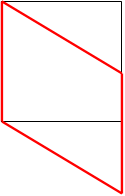
\includegraphics[height=4cm]{simple-shear}
	\caption{Simple shear}
	\label{fig:simple-shear}
\end{figure}

\begin{itemize}
	\item černá je nedeformovaná geometrie
	\item červená je deformovaná geometrie
	\item třetí rozměr zůstává bez změny ($\lambda_3 = 1$)
	\item volumetrická změna $= 0$
	\item pozor: indukují se i normálová napětí (při velkých -- \uv{neinfinitezimálních} -- deformacích)
	\item hlavní osy tenzoru deformace se v průběhu vzrůstající úrovně deformace NATÁČEJÍ
\end{itemize}

Praktická realizace:
\begin{figure}[H]
	\centering
	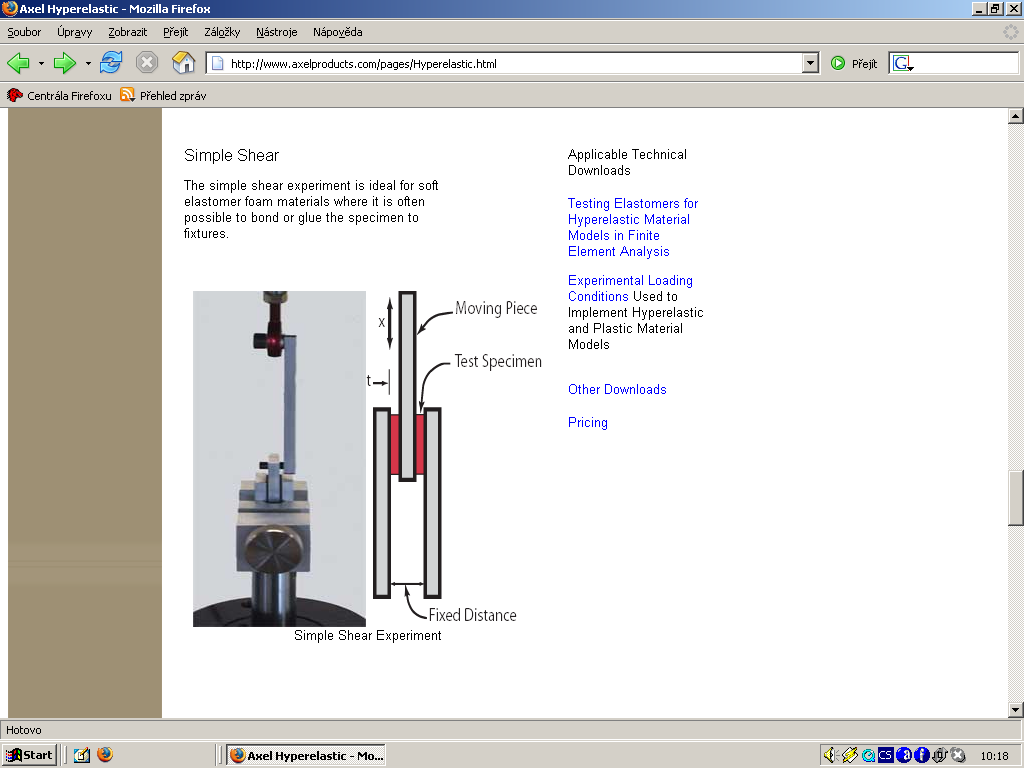
\includegraphics[width=0.4\linewidth]{Obrazky/simple-shear-experiment}
	\caption{Simple shear experiment}
	\label{fig:simple-shear-experiment}
\end{figure}

\subsubsection{Pure shear}
\begin{figure}[H]
	\centering
	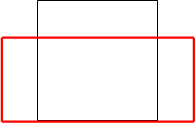
\includegraphics[height=4cm]{pure-shear}
	\caption{Pure shear}
	\label{fig:pure-shear}
\end{figure}

\begin{itemize}
	\item třetí rozměr zůstává bez změny ($\lambda_3 = 1$)
	\item volumetrická změna $= 0$ (v~praxi při tzv. \uv{pure shear} testu není většinou splněno)
	\item praktická realizace: tahem v~širokých čelistech na širokém vzorku nebo tlakem hranolového vzorku při zabránění jedné z~příčných deformací
\item hlavní osy deformace se v~průběhu vzrůstající úrovně deformace nenatáčí
\end{itemize}

\subsubsection{Vysvětlení vzájemné ekvivalence}
\begin{figure}[H]
	\centering
	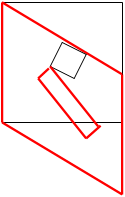
\includegraphics[height=4cm]{shear-vzajemna-ekvivalence}
	\caption{Vzajemná ekvivalence}
	\label{fig:shear-vzajemna-ekvivalence}
\end{figure}

Na případu „simple shear“ lze pro danou úroveň deformace (gama) vždy nalézt na deformovaném vzorku ortogonální (pravoúhlý) element, kterému v nedeformované konfiguraci odpovídá rovněž ortogonální element. Tedy na takovém elementu neproběhl smyk vůči jeho hranám -- element se pouze cely natočil, v jednom směru natáhl a~v~druhém stlačil (volumetrická změna $= 0$). Stav deformace pro tento element je z~podstaty věci ekvivalentní stavu „pure shear“. Jediný rozdíl je v NATÁČENÍ hlavních os deformace,  proto také zápis obou typů deformací do podoby deformačního gradientu je vzájemně odlišný -- deformační gradient obsahuje totiž i~rotaci tělesa („rigid body rotation“).

% !TeX root = skripta-konstitutivni-vztahy.tex
% !TeX lastmodified = 2013-10-30

\subsection{Co jsou to konečné deformace?}
Termínem konečné deformace (finite strain) označujeme přetvoření, která na rozdíl od klasické teorie pružnosti nejsou nekonečně malá (infinitezimální).
V~praxi lze teorie založené na předpokladu malých (infinitezimálních, tedy nekonečně malých) přetvoření používat, pokud přetvoření nepřesáhnou cca 1\%.
V~opačném případě je třeba používat teorie konečných (rozuměj nikoli nekonečně malých, tedy vlastně velkých) přetvoření.

% !TeX root = skripta-konstitutivni-vztahy.tex
% !TeX lastmodified = 2006-11-04

\subsection{Označení deformovaných a~nedeformovaných souřadnic}

\begin{figure}[H]
	\centering
	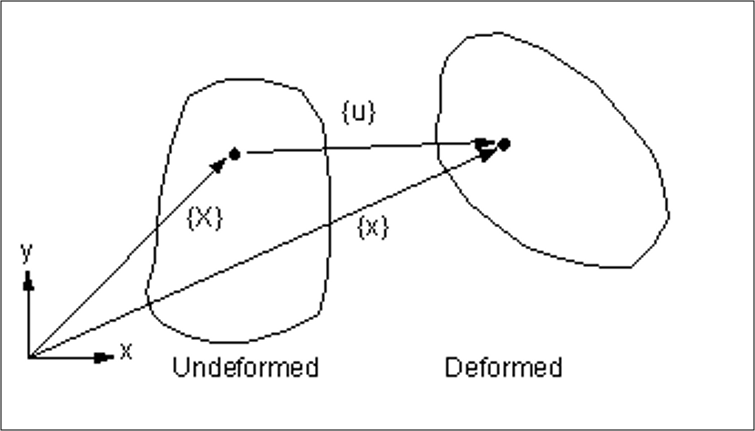
\includegraphics[width=0.7\linewidth]{deformovane-nedeformovane-souradnice}
	\caption{Souřadnice}
	\label{fig:deformovane-nedeformovane-souradnice}
\end{figure}

% !TeX root = ../skripta-konstitutivni-vztahy-materialu.tex

\section{Maticový zápis tenzorů}
Symetrický tenzor druhého řádu $3 \times 3$ se složkami $i,j \in \{1,2,3\}$ lze zapsat jako vektor se složkami $a \in \{1,2,3,4,5,6\}$
\begin{equation*}
	T_{ij} =
	\begin{pmatrix}
		T_{11} & T_{12} & T_{13} \\ & T_{22} & T_{23} \\ \text{\small sym.} & & T_{33} \\
	\end{pmatrix}
	\quad\rightarrow\quad
	T_a =
	\begin{pmatrix}
		T_1 \\ T_2 \\ T_3 \\ T_4 \\ T_5 \\ T_6 \\
	\end{pmatrix}
\end{equation*}
a~symetrický tenzor čtvrtého řádu $3 \times 3 \times 3 \times 3$ se složkami $i,j,k,l \in \{1,2,3\}$ lze zapsat jako matici $6 \times 6$ se složkami $a,b \in \{1,2,3,4,5,6\}$
\begin{equation*}
	T_{ijkl}
	\quad\rightarrow\quad
	T_{ab} =
	\begin{pmatrix}
		T_{11} & T_{12} & T_{13} & T_{14} & T_{15} & T_{16} \\
		& T_{22} & T_{23} & T_{24} & T_{25} & T_{26} \\
		& & T_{33} & T_{34} & T_{35} & T_{36} \\
		& & & T_{44} & T_{45} & T_{46} \\
		& \text{\small sym.} & & & T_{55} & T_{56} \\
		& & & & & T_{66} \\
	\end{pmatrix}
\end{equation*}

Při zápisu tenzoru napětí a~tenzoru přetvoření pomocí vektorů je potřeba zachovat hodnotu hustoty elastické energie, která je produktem $2E = \bm{\sigma}\kontr\bm{\varepsilon} = \{\sigma\}^T\cdot\{\varepsilon\}$. Tradiční Voigtův\footnote{Woldemar \textsc{Voigt} (Němec, 1850---1919)} zápis i~méně používaný Kelvinův\footnote{William \textsc{Thomson} -- lord Kelvin (Skot, 1824---1907)}-Mandelův\footnote{Jean \textsc{Mandel} (Francouz, 1907-1982)} zápis toho dosahují různými mapováními.

\subsection{Voigtův zápis}
Tenzor napětí
\begin{equation*}
	\sigma_{ij} =
	\begin{pmatrix}
		\sigma_{11} & \sigma_{12} & \sigma_{13} \\ & \sigma_{22} & \sigma_{23} \\ \text{sym.} & & \sigma_{33} \\
	\end{pmatrix} =
	\begin{pmatrix}
		\sigma_{11} & \tau_{12} & \tau_{13} \\ & \sigma_{22} & \tau_{23} \\ \text{sym.} & & \sigma_{33} \\
	\end{pmatrix}
	\quad\rightarrow\quad
	\sigma_a =
	\begin{pmatrix}
		\sigma_{11} \\ \sigma_{22} \\ \sigma_{33} \\ \sigma_{23} \\ \sigma_{13} \\ \sigma_{12} \\
	\end{pmatrix} =
	\begin{pmatrix}
		\sigma_{11} \\ \sigma_{22} \\ \sigma_{33} \\ \tau_{23} \\ \tau_{13} \\ \tau_{12} \\
	\end{pmatrix}
\end{equation*}

Tenzor přetvoření
\begin{equation*}
	\varepsilon_{ij} =
	\begin{pmatrix}
		\varepsilon_{11} & \varepsilon_{12} & \varepsilon_{13} \\ & \varepsilon_{22} & \varepsilon_{23} \\ \text{\small sym.} & & \varepsilon_{33} \\
	\end{pmatrix} =
	\begin{pmatrix}
		\varepsilon_{11} & \frac{\gamma_{12}}{2} & \frac{\gamma_{13}}{2} \\ & \varepsilon_{22} & \frac{\gamma_{23}}{2} \\ \text{\small sym.} & & \varepsilon_{33} \\
	\end{pmatrix}
	\quad\rightarrow\quad
	\varepsilon_{a} =
	\begin{pmatrix}
		\varepsilon_{11} \\ \varepsilon_{22} \\ \varepsilon_{33} \\ 2 \varepsilon_{23} \\ 2 \varepsilon_{13} \\ 2 \varepsilon_{12} \\
	\end{pmatrix} =
	\begin{pmatrix}
		\varepsilon_{11} \\ \varepsilon_{22} \\ \varepsilon_{33} \\ \gamma_{23} \\ \gamma_{13} \\ \gamma_{12} \\
	\end{pmatrix}
\end{equation*}

Tenzor tuhosti
\begin{equation*}
	C_{ijkl}
	\quad\rightarrow\quad
	C_{ab} =
	\begin{pmatrix}
	C_{1111} & C_{1122} & C_{1133} & C_{1123} & C_{1113} & C_{1112} \\
	         & C_{2222} & C_{2233} & C_{2223} & C_{2213} & C_{2212} \\
	         &          & C_{3333} & C_{3323} & C_{3313} & C_{3312} \\
	         &          &          & C_{2323} & C_{2313} & C_{2312} \\
	      & \text{\small sym.} &          &          & C_{1313} & C_{1112} \\
	         &          &          &          &          & C_{1212} \\
	\end{pmatrix}
\end{equation*}

Výhody:
\begin{itemize}
	\item zachování hustoty elastické energie
	\item zachování složek tenzoru tuhosti
\end{itemize}

Nevýhody:
\begin{itemize}
	\item napětí a~přetvoření je mapováno různými způsoby
	\item norma tenzorů se nezachovává
\end{itemize}

\subsection{Kelvinův-Mandelův zápis}
Tenzor napětí
\begin{equation*}
\sigma_{ij} =
\begin{pmatrix}
\sigma_{11} & \sigma_{12} & \sigma_{13} \\ & \sigma_{22} & \sigma_{23} \\ \text{sym.} & & \sigma_{33} \\
\end{pmatrix} =
\begin{pmatrix}
\sigma_{11} & \tau_{12} & \tau_{13} \\ & \sigma_{22} & \tau_{23} \\ \text{sym.} & & \sigma_{33} \\
\end{pmatrix}
\quad\rightarrow\quad
\sigma_a =
\begin{pmatrix}
\sigma_{11} \\ \sigma_{22} \\ \sigma_{33} \\ \sqrt{2} \sigma_{23} \\ \sqrt{2} \sigma_{13} \\ \sqrt{2} \sigma_{12} \\
\end{pmatrix} =
\begin{pmatrix}
\sigma_{11} \\ \sigma_{22} \\ \sigma_{33} \\ \sqrt{2} \tau_{23} \\ \sqrt{2} \tau_{13} \\ \sqrt{2} \tau_{12} \\
\end{pmatrix}
\end{equation*}

Tenzor přetvoření
\begin{equation*}
\varepsilon_{ij} =
\begin{pmatrix}
\varepsilon_{11} & \varepsilon_{12} & \varepsilon_{13} \\ & \varepsilon_{22} & \varepsilon_{23} \\ \text{\small sym.} & & \varepsilon_{33} \\
\end{pmatrix} =
\begin{pmatrix}
\varepsilon_{11} & \frac{\gamma_{12}}{2} & \frac{\gamma_{13}}{2} \\ & \varepsilon_{22} & \frac{\gamma_{23}}{2} \\ \text{\small sym.} & & \varepsilon_{33} \\
\end{pmatrix}
\quad\rightarrow\quad
\varepsilon_{a} =
\begin{pmatrix}
\varepsilon_{11} \\ \varepsilon_{22} \\ \varepsilon_{33} \\ \sqrt{2} \varepsilon_{23} \\ \sqrt{2} \varepsilon_{13} \\ \sqrt{2} \varepsilon_{12} \\
\end{pmatrix} =
\begin{pmatrix}
\varepsilon_{11} \\ \varepsilon_{22} \\ \varepsilon_{33} \\ \frac{\sqrt{2}}{2} \gamma_{23} \\ \frac{\sqrt{2}}{2} \gamma_{13} \\ \frac{\sqrt{2}}{2} \gamma_{12} \\
\end{pmatrix}
\end{equation*}

Tenzor tuhosti
\begin{equation*}
C_{ijkl}
\quad\rightarrow\quad
C_{ab} =
\begin{pmatrix}
C_{1111} & C_{1122} & C_{1133} & \sqrt{2} C_{1123} & \sqrt{2} C_{1113} & \sqrt{2} C_{1112} \\
& C_{2222} & C_{2233} & \sqrt{2} C_{2223} & \sqrt{2} C_{2213} & \sqrt{2} C_{2212} \\
&          & C_{3333} & \sqrt{2} C_{3323} & \sqrt{2} C_{3313} & \sqrt{2} C_{3312} \\
&          &          & 2 C_{2323} & 2 C_{2313} & 2 C_{2312} \\
& \text{\small sym.} &          &          & 2 C_{1313} & 2 C_{1112} \\
&          &          &          &          & 2 C_{1212} \\
\end{pmatrix}
\end{equation*}

Výhody:
\begin{itemize}
	\item zachování hustoty elastické energie
	\item zachování normy tenzorů
	\item napětí a~přetvoření je mapováno stejným způsobem
\end{itemize}

Nevýhody:
\begin{itemize}
	\item složky tenzoru tuhosti se nezachovávají
\end{itemize}


\section{Tenzory deformace}
% !TeX root = skripta-konstitutivni-vztahy.tex
% !TeX lastmodified = 2014-11-10

\subsection{Tenzor deformačního gradientu}
Složkami tenzoru deformačního gradientu $\bm{F}$ jsou poměrná protažení
\begin{equation}
	\lambda_x  = \frac{\partial x}{\partial X}
	\qquad
	\lambda_y  = \frac{\partial y}{\partial Y}
	\qquad
	\lambda_z  = \frac{\partial z}{\partial Z}
\end{equation}

Obecně je lze zapsat ve tvaru
\begin{equation}
	\lambda_{ij}  = \frac{\partial x_i}{\partial X_j}
\end{equation}

Úplný maticový zápis v obecném souřadnicovém systému je
\begin{equation}
	\bm{F} = \left(\begin{matrix}
		\frac{\partial x_1}{\partial X_1} & \frac{\partial x_1}{\partial X_2} & \frac{\partial x_1}{\partial X_3}\\
		\frac{\partial x_2}{\partial X_1} & \frac{\partial x_2}{\partial X_2} & \frac{\partial x_2}{\partial X_3}\\
		\frac{\partial x_3}{\partial X_1} & \frac{\partial x_3}{\partial X_2} & \frac{\partial x_3}{\partial X_3}
	\end{matrix}\right)
\end{equation}

Třetí invariant tenzoru deformačního gradientu je dán determinantem této matice $\bm{F}$, který lze nejsnáze určit z~hlavních hodnot poměrných protažení pomocí vztahu
\begin{equation}
	J = \det(\bm{F}) = \lambda_1 \lambda_2 \lambda_3
\end{equation}

\subsubsection{Vlastnosti tenzoru deformačního gradientu}
Tenzor deformačního gradientu je obecně nesymetrický, v~důsledku toho existují dva v~principu odlišné Cauchy-Greenovy tenzory deformace (levý a~pravý).

Třetí invariant $J$ tenzoru deformačního gradientu $\bm{F}$ udává poměrnou objemovou změnu elementu, jak plyne z následujícího vztahu: 
\begin{equation}
	e
	= \frac{V_\text{def} - V_\text{nedef}}{V_\text{nedef}}
	= \frac{\diff x \diff y \diff z - \diff X \diff Y \diff Z}{\diff X \diff Y \diff Z}
	= \frac{\partial x}{\partial X} \frac{\partial y}{\partial Y} \frac{\partial z}{\partial Z} - 1
	= \lambda_1 \lambda_2 \lambda_3 -1
	= J - 1
\end{equation}

Jako každý tenzor lze i~tenzor deformačního gradientu tedy rozložit na část kulovou (změna objemu) a~deviátorovou (změna tvaru). 

U~smluvních přetvoření byla kulová část tenzoru dána aritmetickým průměrem hlavních přetvoření. Podobně zde je kulová část dána průměrem hlavních souřadnic tenzoru, ovšem nikoli aritmetickým, nýbrž geometrickým, protože změna objemu je dána součinem těchto souřadnic.

Pro střední protažení platí tedy
\begin{equation}
	\lambda_s
	= \sqrt[3]{\lambda_1 \lambda_2 \lambda_3}
	= \sqrt[3]{J}
	= J^{\frac{1}{3}}
\end{equation}




% !TeX root = skripta-konstitutivni-vztahy.tex
% !TeX lastmodified = 2017-10-19

\subsection{Cauchy-Greenův tenzor deformace}
Tato definice nepracuje s~přetvořeními, ale s~poměrnými protaženími, podobně jako tenzor deformačního gradientu $\bm{F}$, z~nějž se odvozuje pomocí vztahů:

Pravý Cauchy-Greenův tenzor deformace
\begin{equation}
	\bm{C} = \bm{F}^T \bm{F}
	\quad\Leftrightarrow\quad
	C_{ij} = F_{ki} F_{kj}
\end{equation}
Levý Cauchy-Greenův tenzor deformace
\begin{equation}
	\bm{B} = \bm{F} \bm{F}^T
	\quad\Leftrightarrow\quad
	B_{ij} = F_{ik} F_{jk}
\end{equation}

Hlavními souřadnicemi tohoto tenzoru jsou kvadráty poměrných protažení v~hlavních směrech
\begin{equation}
	\bm{C} = \left(\begin{matrix}
		\lambda_1^2 & 0 & 0\\
		0 & \lambda_2^2 & 0\\
		0 & 0 & \lambda_3^2
	\end{matrix}\right)
\end{equation}

\subsubsection{Invarianty Cauchy-Greenova tenzoru deformace}
Invarianty tohoto tenzoru lze v hlavním souřadnicovém systému vyjádřit následovně:
\begin{align}
	I_1 &= \lambda_1^2 + \lambda_2^2 + \lambda_3^2\\
	I_2 &= \lambda_1^2 \lambda_2^2 + \lambda_2^2 \lambda_3^2 + \lambda_3^2 \lambda_1^2\\
	I_3 &= \lambda_1^2 \lambda_2^2 \lambda_3^2 = J^2
\end{align}

Zde $J$ je třetí invariant tenzoru deformačního gradientu. Třetí invariant tedy i~u~Cauchy-Greenova tenzoru deformace vyjadřuje změnu objemu (je roven jedné, pokud se při deformaci objem nemění).

Tenzorový zápis těchto invariantů je následující
\footnote{*G.A.Holzapfel:Nonlinear solid mechanics. Wiley, 2001, p. 25.}
\begin{align}
	I_1 &= \mathrm{Sp}(\bm{C})%todo zarovnání
	&\quad\Leftrightarrow\quad
	I_1 &= C_{ii}\\
	I_2 &= \frac{1}{2} \left[\mathrm{Sp}(\bm{C})^2 - \mathrm{Sp}(\bm{C}^2)\right]
	&\quad\Leftrightarrow\quad
	I_2 &= \frac{1}{2} (C_{ii} C_{jj} - C_{ij} C_{ji})\\
	I_3 &= \det(\bm{C})
\end{align}

%\subsubsection{Modifikované invarianty Cauchy-Greenova tenzoru deformace}
%Ve vztazích pro funkce měrné energie napjatosti se obvykle používají tzv. modifikované hodnoty hlavních poměrných protažení, které vyjadřují pouze tvarovou (deviátorovou) část tenzoru deformace, a~z~nich odvozené modifikované invarianty Cauchy-Greenova tenzoru deformace:
%\begin{align}
%	\bar{I}_1 &= \bar{\lambda}_1^2 + \bar{\lambda}_2^2 + \bar{\lambda}_3^2\\
%	\bar{I}_2 &= \bar{\lambda}_1^2 \bar{\lambda}_2^2 +\bar{ \lambda}_2^2 \bar{\lambda}_3^2 + \bar{\lambda}_3^2 \bar{\lambda_1}^2\\
%	I_3 &= \bar{\lambda}_1^2 \bar{\lambda}_2^2 \bar{\lambda}_3^2 = 1
%\end{align}

\subsubsection{Modifikované invarianty Cauchy-Greenova tenzoru deformace}
Modifikované (též někdy označované jako redukované) invarianty Cauchy-Greenova tenzoru deformace se ve vztazích pro funkce měrné energie napjatosti používají pro popis deviátorové složky deformace. Tak jako deviátor tenzoru malých přetvoření vznikl odečtením středního přetvoření od jednotlivých složek délkových přetvoření, zde dostaneme příslušná poměrná protažení dělením jednotlivých složek středním protažením $\lambda_s$. 

Pak dostaneme modifikovaná hlavní protažení z~rovnice
\begin{equation}
\bar{\lambda}_p = J^{-\frac{1}{3}} \lambda_p \quad (p = 1,2,3)
\end{equation}

Modifikované invarianty Cauchy-Greenova tenzoru deformace jsou pak dány
\begin{align}
\bar{I}_1
&= \bar{\lambda}_1^2 + \bar{\lambda}_2^2 + \bar{\lambda}_3^2
= \left(\lambda_1^2 + \lambda_2^2 + \lambda_3^2\right) J^{-\frac{2}{3}}
= I_1 J^{-\frac{2}{3}}
= I_1 I_3^{-\frac{1}{3}}\\
\bar{I}_2
&= \bar{\lambda}_1^2 \bar{\lambda}_2^2 + \bar{\lambda}_2^2 \bar{\lambda}_3^2 + \bar{\lambda}_1^2 \bar{\lambda}_3^2
= \left(\lambda_1^2 \lambda_2^2 + \lambda_2^2 \lambda_3^2 + \lambda_1^2 \lambda_3^2\right) J^{-\frac{4}{3}}
= I_2 J^{-\frac{4}{3}}
= I_2 I_3^{-\frac{2}{3}}
\end{align}

% !TeX root = skripta-konstitutivni-vztahy-materialu.tex
% !TeX lastmodified = 2019-11-27

\subsection{Tenzor protažení (stretch tensor)}
I~v~nedeformovaném stavu elementu může mít matice definující tenzor deformačního gradientu $\bm{F}$ složky odlišné od jednotkové matice; je to dáno případnou rotací elementu v~důsledku velkých deformací tělesa.  Polární dekompozicí tenzoru $\bm{F}$ lze tento rozložit na tenzor rotace $\bm{R}$ (vyjadřující rotaci tuhého tělesa) a~tenzor protažení $\bm{U}$ nebo $\bm{V}$ (popisující deformaci tělesa). Tento tenzor je již symetrický a~energeticky konjugovaný se symetrickou částí Biotova tenzoru napětí $\bm{T_B}$. 

Tenzor deformačního gradientu je definován vztahem
\begin{equation}
	F_{iJ} := \frac{\partial x_i}{\partial X_J}
\end{equation}
který můžeme přepsat do maticové podoby s~konečnými diferencemi namísto derivací
\begin{equation}
	\bm{F} = \frac{\Delta \bm{x}}{\Delta \bm{X}}
\end{equation}

Polární dekompozice tenzoru $\bm{F}$ pak spočívá v~jeho rozložení na tenzor 
rotace $\bm{R}$ a~pravý nebo levý tenzor protažení (stretch tensor) $\bm{U}$ nebo $\bm{V}$:
\begin{equation}
	\bm{F} = \bm{R} \bm{U} = \bm{V} \bm{R}
	\quad\Rightarrow\quad
	\bm{U} = \bm{R}^{-1} \bm{F} = \bm{R}^T \bm{F};
	\quad
	\bm{V} = \bm{F} \bm{R}^{-1} = \bm{F} \bm{R}^T
\end{equation}
Zde se využívá ortogonality tenzoru rotace $\bm{R}$, pro který tedy inverzní matice se rovná matici transponované.

Tenzor rotace $\bm{R}$ je v rovině (2D zjednodušení) definován vztahem
\begin{equation}
	\bm{R} = \left(\begin{matrix}
		\cos(\psi) & \sin(\psi)\\
		-\sin(\psi) & \cos(\psi)\\
	\end{matrix}\right),
\end{equation}
kde úhel $\psi$ lze určit ze složek tenzoru deformačního gradientu pomocí vztahu
\begin{equation}
	\psi = \arctan\left(\frac{F_{12} - F_{21}}{F_{11} + F_{22}}\right)
\end{equation}

Pomocí tenzorů protažení $\bm{U}$ a~$\bm{V}$ lze pak definovat také Cauchyho-Greenův tenzor deformace $C$ a~Fingerův tenzor deformace $\bm{B}$ pomocí vztahů:
\begin{equation}
	\bm{C} = \bm{F}^T \bm{F} = \bm{U}^T \bm{U} = U^2; \quad
	\bm{B} = \bm{F} \bm{F}^T = \bm{V} \bm{V}^T = V^2; \quad
\end{equation}
Zde se navíc využívá faktu, že oba tyto tenzory jsou (na rozdíl od tenzoru deformačního gradientu $\bm{F}$) vždy symetrické. Hlavní složky tenzoru $\bm{U}$ i~$\bm{V}$ jsou stejné a představují hlavní poměrná protažení (principal stretches). 


\section{Tenzory přetvoření}
% !TeX root = skripta-konstitutivni-vztahy.tex
% !TeX lastmodified = 2006-11-04

\begin{figure}[H]
	\centering
	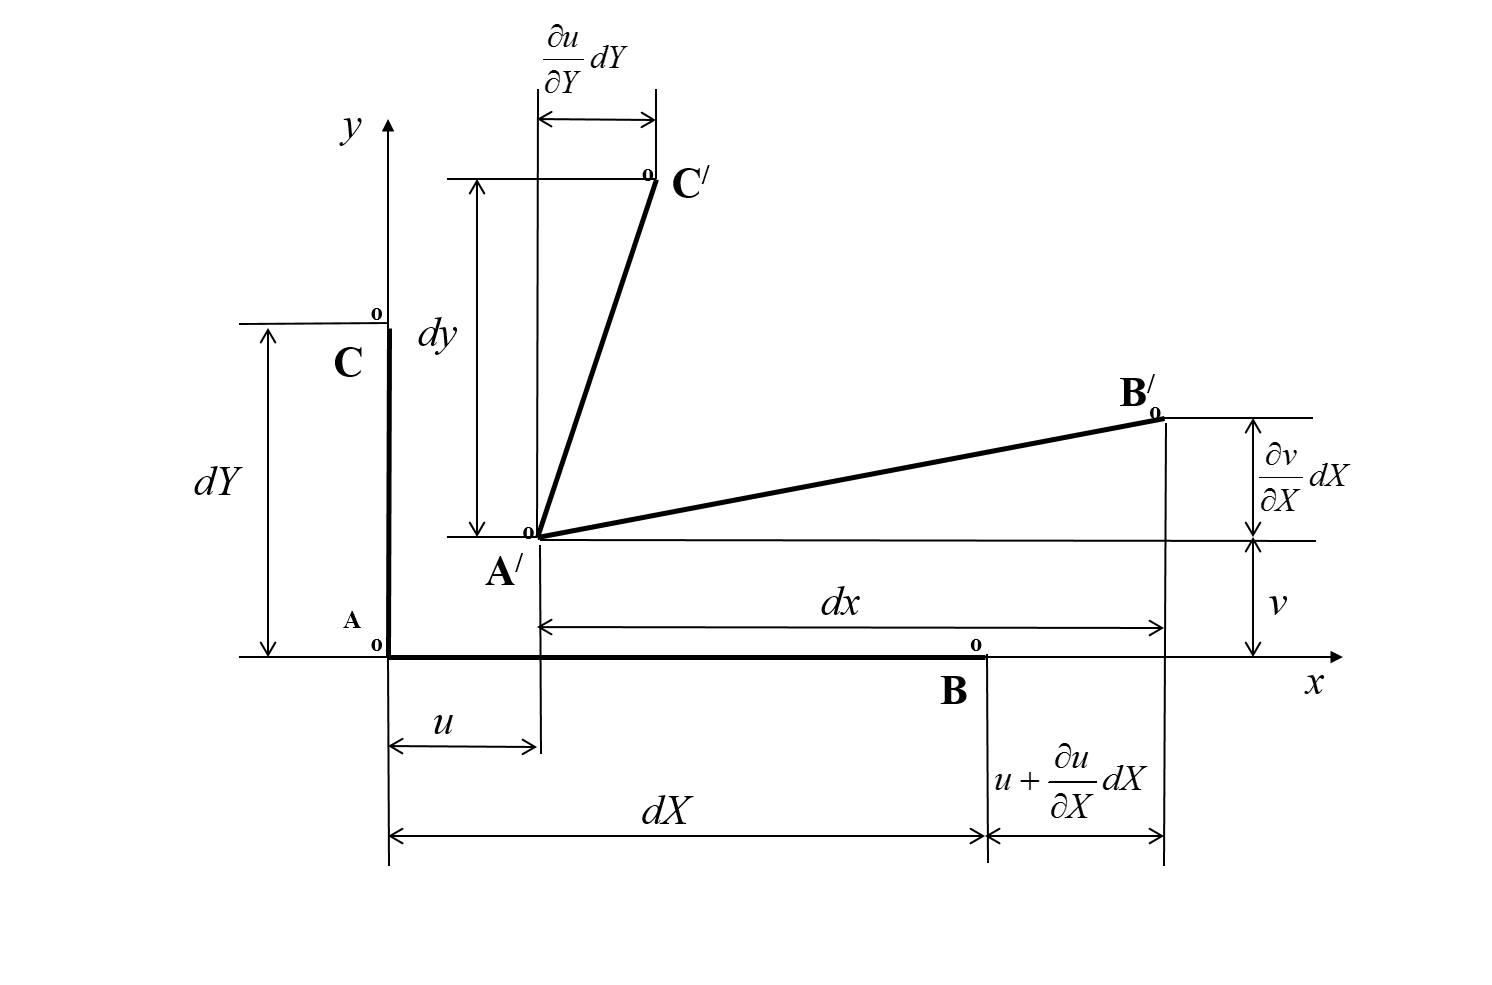
\includegraphics[width=0.7\linewidth]{pretvoreni}
	\caption{Přetvoření}
	\label{fig:pretvoreni}
\end{figure}

% !TeX root = skripta-konstitutivni-vztahy.tex
% !TeX lastmodified = 2006-11-05

\subsection{Tenzor smluvního přetvoření (pro malé deformace)}
Délková (označení viz obrázek \ref{fig:pretvoreni}):
\begin{equation}
	\varepsilon_x
	= \frac{\diff x - \diff X}{\diff X}
	= \frac{\diff X + u + \frac{\partial u}{\partial X}\diff X - u - \diff X}{\diff X}
	= \frac{\partial u}{\partial X}
\end{equation}

Pro ostatní složky analogicky:
\begin{equation}
	\varepsilon_x
	= \frac{\partial v}{\partial Y}
	\qquad
	\varepsilon_z
	= \frac{\partial w}{\partial Z}
\end{equation}

Úhlová (zkosy):
\begin{equation}
	\gamma_{xy}
	= \gamma_{AB} + \gamma_{AC}
	= \tan(\gamma_{AB}) + \tan(\gamma_{AB})
	= \frac{\frac{\partial v}{\partial X} \diff X}{\diff X}
	+ \frac{\frac{\partial u}{\partial Y} \diff Y}{\diff Y}
	= \frac{\partial v}{\partial X} + \frac{\partial u}{\partial Y}
\end{equation}

Pro ostatní složky analogicky:
\begin{equation}
	\gamma_{yz}
	= \frac{\partial v}{\partial Z} + \frac{\partial w}{\partial Y}
	\qquad
	\gamma_{xz}
	= \frac{\partial u}{\partial Z} + \frac{\partial w}{\partial X}
\end{equation}

Vzhledem k tomu, že složkami tenzoru přetvoření jsou poloviční zkosy, lze napsat obecný tenzorový vztah
\begin{equation}
	\bm{\varepsilon} := \tfrac{1}{2} \left( \nabla\bm{u} + \nabla^T\bm{u} \right)
	\quad\Leftrightarrow\quad
	\varepsilon_{ij} := \frac{1}{2} \left( \frac{\partial u_i}{\partial X_j} + \frac{\partial u_j}{\partial X_i} \right),
\end{equation}
kde souřadnicím $X$, $Y$, $Z$ odpovídají $X_i$ a~posuvům $u$, $v$, $w$ posuvy $u_i$ (pro $i=1,2,3$).

% !TeX root = skripta-konstitutivni-vztahy.tex
% !TeX lastmodified = 2019-10-23

\subsection{Tenzor Greenova-Lagrangeova přetvoření}\label{sec:green-lagrange}
Přetvoření (poměrná deformace) je rovněž vztažena k původním (nedeformovaným) rozměrům, ale je respektováno i natáčení elementu. Pak je délkové přetvoření (označení viz obrázek \ref{fig:pretvoreni}):
\begin{equation}\begin{split}
	E^L_x &= \frac{A'B' - AB}{AB}
	= \frac{\sqrt{\diff x^2 + \left( \frac{\partial v}{\partial X} \diff X \right)^2 + \left( \frac{\partial w}{\partial X} \diff X \right)^2} - \diff X}{\diff X}\\
	&= \frac{\sqrt{ \left( \diff X + u + \frac{\partial u}{\partial X} \diff X - u \right)^2 + \left( \frac{\partial v}{\partial X} \diff X \right)^2 + \left( \frac{\partial w}{\partial X} \diff X \right)^2} - \diff X}{\diff X}
\end{split}\end{equation}

Deformovaná délka elementu dx se zde počítá aplikací Pythagorovy věty ve 3D prostoru (není v obrázku zakresleno). Pro zjednodušení vztahu použijeme první dva členy binomické řady:
\begin{equation}
	\sqrt{1 + \kappa} = 1 + \frac{\kappa}{2} - \frac{\kappa^2}{8} + \frac{\kappa^3}{16} - \ldots
\end{equation}
Pak dostaneme:
\begin{equation}\begin{split}
	E^L_x
	&= \frac{\diff X \sqrt{ 1 + 2 \frac{\partial u}{\partial X} + \left( \frac{\partial u}{\partial X} \right)^2 + \left( \frac{\partial v}{\partial X} \right)^2 + \left( \frac{\partial w}{\partial X} \right)^2} - \diff X}{\diff X}\\
	&= 1 + \frac{2 \frac{\partial u}{\partial X} + \left( \frac{\partial u}{\partial X} \right)^2 + \left( \frac{\partial v}{\partial X} \right)^2 + \left( \frac{\partial w}{\partial X} \right)^2}{2} - 1\\
	&= \frac{\partial u}{\partial X} + \frac{1}{2} \left[ \left( \frac{\partial u}{\partial X} \right)^2 + \left( \frac{\partial v}{\partial X} \right)^2 + \left( \frac{\partial w}{\partial X} \right)^2 \right]
\end{split}\end{equation}
Pro ostatní složky délkových přetvoření platí analogicky:
\begin{equation}\begin{split}
	E^L_y
	&= \frac{\partial v}{\partial Y} + \frac{1}{2} \left[ \left( \frac{\partial u}{\partial Y} \right)^2 + \left( \frac{\partial v}{\partial Y} \right)^2 + \left( \frac{\partial w}{\partial Y} \right)^2 \right]\\
	E^L_z
	&= \frac{\partial w}{\partial Z} + \frac{1}{2} \left[ \left( \frac{\partial u}{\partial Z} \right)^2 + \left( \frac{\partial v}{\partial Z} \right)^2 + \left( \frac{\partial w}{\partial Z} \right)^2 \right]
\end{split}\end{equation}

Zobecnění na všechny složky tenzoru přetvoření je možné pomocí tenzorového zápisu
\begin{equation}
	E^L_{ij}
	= \frac{1}{2} \left[ \frac{\partial u_i}{\partial X_j} + \frac{\partial u_j}{\partial X_i} + \frac{\partial u_k}{\partial X_j} \frac{\partial u_k}{\partial X_i} \right]
\end{equation}
Tento zápis používá Einsteinovo sčítací pravidlo.

% !TeX root = skripta-konstitutivni-vztahy.tex
% !TeX lastmodified = 2019-10-23

\subsection{Tenzor Almansiho-Hamelova přetvoření}
Podle Almansiho se poměrné přetvoření vztahuje ke konečným (nedeformovaným) rozměrům. Pak délkové přetvoření lze vyjádřit (označení viz obrázek \ref{fig:pretvoreni}):
\begin{equation}
	E^A_x = \frac{A'B' - AB}{A'B'}
\end{equation}

Podobným postupem jako pro tenzor Greenova-Lagrangeova přetvoření se dospěje k obecnému tenzorovému zápisu ve tvaru:
\begin{equation}
	E^A_{ij}
	= \frac{1}{2} \left[ \frac{\partial u_i}{\partial x_j} + \frac{\partial u_j}{\partial x_i} - \frac{\partial u_k}{\partial x_j} \frac{\partial u_k}{\partial x_i} \right]
\end{equation}
Také tento zápis používá Einsteinovo sčítací pravidlo.

Praktické použití tohoto tenzoru je omezeno tím, že konečné (deformované) souřadnice obvykle předem neznáme.

% !TeX root = skripta-konstitutivni-vztahy.tex
% !TeX lastmodified = 2016-10-10

\subsection{Cauchyho (logaritmický) tenzor přetvoření}
Nedostatky tenzorů konečných přetvoření:
\begin{itemize}
	\item Green-Lagrange: změny délek jsou stále vztahovány k~původním hodnotám, zatímco aktuální již mohou být v průběhu procesu zatěžování významně odlišné.
	\item Almansi-Hamel: změny délek jsou stále vztahovány ke konečným (deformovaným) hodnotám délek, zatímco aktuální od nich mohou být v~průběhu procesu zatěžování ještě podstatně odlišné.
\end{itemize}

Cauchyho definice přetvoření je exaktnější v~tom, že infinitezimální přírůstek délky vztahuje vždy k~aktuální délce v~daném stádiu zatěžovacího procesu.

Přetvoření úsečky o~původní délce $X_{i0}$, která se vlivem zatížení mění na aktuální hodnotu $X_i$ až dosáhne konečné (deformované) délky $x_{ik}$, určíme integrací přírůstků její délky $\diff x_i$:
\begin{equation}
	E^C_{ij}
	= \int\limits_{X_{i0}}^{x_{ik}} \frac{1}{x_i} \diff x_i
	= \left. \ln(x) \right\rvert_{X_{i0}}^{x_{ik}}
	= \ln(x_{ik}) - \ln(X_{i0})
	= \ln\left(\frac{x_{ik}}{X_{i0}}\right)
	= \ln(\lambda_i)
\end{equation}

\subsubsection{Tenzorová formulace Cauchyho tenzoru přetvoření}

Složky tohoto tenzoru jsou rovny přirozeným logaritmům odpovídajících složek tenzoru deformačního gradientu.


Souřadnice tohoto tenzoru jsou tedy rovny přirozeným logaritmům odpovídajících souřadnic tenzoru deformačního gradientu.
\begin{equation}
	E^C_{ij} = \ln(F_{ij}) = \frac{1}{2} \ln(C_{ij})
\end{equation}

% !TeX root = skripta-konstitutivni-vztahy.tex
% !TeX lastmodified = 2016-12-06

\subsection{Vzájemné přepočtové vztahy pro tenzory přetvoření}
Nejvhodnější pro vzájemný přepočet tenzorů přetvoření jsou poměrná protažení $\lambda_i$, tedy složky tenzoru deformačního gradientu. Pro jednoduchost jsou uvedena jen hlavní přetvoření jako funkce hlavních poměrných protažení $\lambda_i$:

Smluvní přetvoření -- vztah se odvozuje v~základní PP: 
\begin{equation}
	\varepsilon_i = \lambda_i - 1
\end{equation}

Green-Lagrange:
\begin{equation}
	E^L_i
	= \frac{\partial u_i}{\partial X_i} + \frac{1}{2} \left(\frac{\partial u_i}{\partial X_i}\right)^2
	= \lambda_i - 1 + \frac{1}{2} (\lambda_i - 1)^2
	= \frac{1}{2} (\lambda_i^2 - 1)
\end{equation}
příp. v~maticovém vyjádření:
\begin{equation}
	\bm{E}^L = \frac{1}{2} \left(\bm{F}^T \bm{F} - \bm{1}\right)
\end{equation}

Almansi-Hamel:
\begin{equation}
	E^A_i
	= \frac{\partial u_i}{\partial x_i} - \frac{1}{2} \left(\frac{\partial u_i}{\partial x_i}\right)^2
	= 1 - \lambda_i^{-1} - \frac{1}{2} (1 - \lambda_i^{-1})^2
	= \frac{1}{2} (1 - \lambda_i^{-2})
\end{equation}

Cauchy:
\begin{equation}
	E^C_i = \ln(\lambda_i)
\end{equation}

\subsubsection{Rozdíly mezi jednotlivými definicemi tenzoru přetvoření}
\begin{figure}[H]
	\centering
	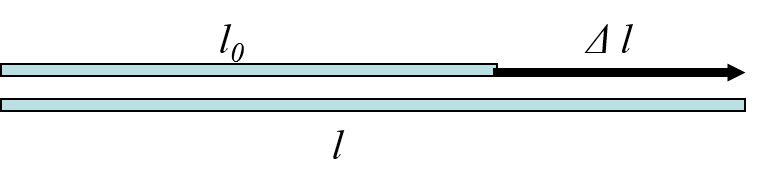
\includegraphics{1d-pretvoreni}
	\caption{Protažení tyče}
	\label{fig:1d-pretvoreni}
\end{figure}

\begin{align}
	E^L &= \frac{1}{2} \frac{l^2 - l_0^2}{l_0^2} = \frac{1}{2} (\lambda^2 - 1)\\
	E^A &= \frac{1}{2} \frac{l^2 - l_0^2}{l^2} = \frac{1}{2} (1 - \lambda^{-2})\\
	\varepsilon &= \frac{l - l_0}{l_0} = \lambda - 1\\
	E^C &= \ln\left(\frac{l}{l_0}\right) = \ln(\lambda)
\end{align}
% Doplnil bych graf v tlaku a řekl které jsou konečné

\begin{figure}[H]
	\centering
	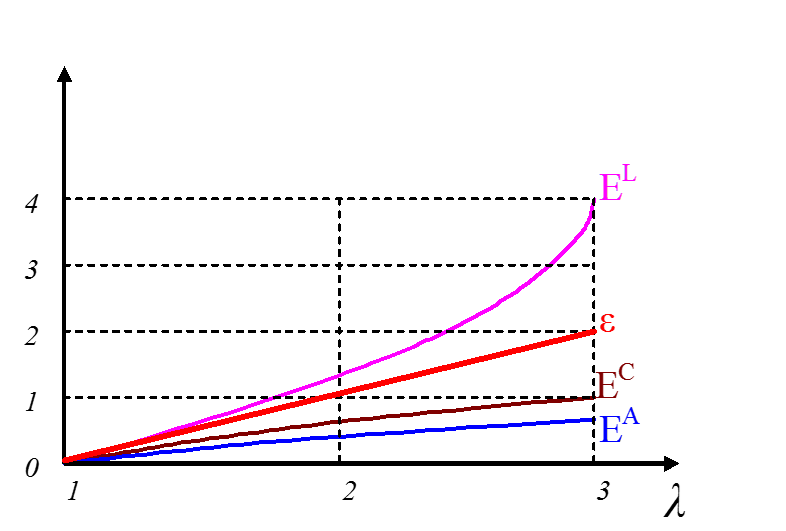
\includegraphics{Obrazky/tenzory-pretvoreni}
	\caption{Přetvoření v tahu}
	\label{fig:tenzory-pretvoreni}
\end{figure}


\section{Tenzory napětí}
% !TeX root = skripta-konstitutivni-vztahy.tex
% !TeX lastmodified = 2019-10-23

\subsection{Tenzor Cauchyho napětí}
Tenzor Cauchyho napětí (v praxi často skutečná napětí -- true stress) je definován jako skutečná elementární síla vztažená na skutečnou (tj. deformovanou) plochu elementu podle vztahu (platí pro hlavní napětí):
\begin{equation}
	\sigma_i = \frac{\diff F_i}{\diff x_j \diff x_k}
\end{equation}
Konkrétně pro hlavní napětí ve směru 1 platí:
\begin{equation}
	\sigma_1 = \frac{\diff F_1}{\diff x_2 \diff x_3}
\end{equation}

% !TeX root = skripta-konstitutivni-vztahy.tex
% !TeX lastmodified = 2006-11-06

\subsection{Piola-Kirchhoffův tenzor napětí 1.~druhu}
1.~Piola-Kirchhoffův tenzor napětí (označovaný také jako Lagrangeův nebo Piolův, v~praxi často smluvní napětí -- engineering stress) je definován jako skutečná elementární síla vztažená na původní (tj. nedeformovanou) plochu elementu podle vztahu (platí pro hlavní napětí):
\begin{equation}
	\tau_i = \frac{\diff F_i}{\diff X_j \diff X_k}
\end{equation}
Konkrétně pro hlavní napětí ve směru 1 platí:
\begin{equation}
	\tau_1 = \frac{\diff F_1}{\diff X_2 \diff X_3}
\end{equation}

% !TeX root = skripta-konstitutivni-vztahy.tex
% !TeX lastmodified = 2010-03-16

\subsection{Piola-Kirchhoffův tenzor napětí 2.~druhu}
2.~Piola-Kirchhoffův (označovaný také jen jako Kirchhoffův) tenzor napětí je definován jako elementární síla $\diff F_{0i}$ vztažená na původní (tj. nedeformovanou) plochu elementu. Tato síla je však při přenášení na původní element změněna oproti skutečné síle $\diff F_i$ stejným poměrem jako elementární rozměr v~odpovídajícím směru. Ten se mění při zatížení podle vztahu
\begin{equation}
	\diff x_i = \frac{\partial x_i}{\partial X_i} \diff X_i,
\end{equation}
resp. při zpětné transformaci do nedeformovaného tvaru
\begin{equation}
	\diff X_i = \frac{\partial X_i}{\partial x_i} \diff x_i.
\end{equation}

Podobně transformujeme i~elementární sílu
\begin{equation}
	\diff F_{0i} = \frac{\partial X_i}{\partial x_i} \diff F_i,
\end{equation}
takže  napětí je
\begin{equation}
	S_i = \frac{\diff F_{0i}}{\diff X_j \diff X_k}
\end{equation}
Konkrétně pro normálové napětí ve směru 1 platí:
\begin{equation}
	S_i = \frac{\diff F_{01}}{\diff X_2 \diff X_3}
	= \frac{\frac{\partial X_1}{\partial x_1} \diff F_1}{\diff X_2 \diff X_3}
\end{equation}

Tento tenzor nemá jasný fyzikální význam, používá se proto, že je i~pro velká přetvoření symetrický a~je energeticky konjugovaný s~Green-Lagrangeovým tenzorem přetvoření.

% !TeX root = skripta-konstitutivni-vztahy.tex
% !TeX lastmodified = 2010-03-16

\subsection{Vzájemné přepočtové vztahy pro tenzory napětí}
Nejvhodnější pro vzájemný přepočet tenzorů přetvoření jsou poměrná protažení $\lambda_i$, tedy složky tenzoru deformačního gradientu. V~hlavním souřadnicovém systému platí následující vztahy:

Hlavní Cauchyho (skutečné) napětí lze vyjádřit pomocí 1.P.K. napětí
\begin{equation}
	\sigma_i = \frac{\diff F_i}{\diff x_j \diff x_k}
	= \frac{\diff F_i}{\lambda_j \diff X_j \lambda_k \diff X_k}
	= \frac{\tau_i}{\lambda_j \lambda_k}
\end{equation}

Pro nestlačitelný materiál platí $\lambda_i\lambda_j\lambda_k=1$ a~tedy napětí jsou ve vztahu
\begin{equation}
	\sigma_i = \frac{\tau_i}{\lambda_j \lambda_k} = \tau_i \lambda_i
\end{equation}

Podobně lze vyjádřit 2.P.K. napětí
\begin{equation}
	S_i = \frac{\diff F_{0i}}{\diff X_j \diff X_k}
	= \frac{\frac{\partial X_i}{\partial x_i} \diff F_i}{\diff X_j \diff X_k}
	= \frac{\frac{1}{\lambda_i} \diff F_i}{\diff X_j \diff X_k}
	= \frac{1}{\lambda_i} \tau_i
\end{equation}

Cauchyho napětí lze vyjádřit i~pomocí 2.P.K. napětí
\begin{equation}
	\sigma_i = \frac{\tau_i}{\lambda_j \lambda_k}
	= \frac{\lambda_i}{\lambda_j \lambda_k} S_i,
\end{equation}
nebo jednodušeji pro nestlačitelný materiál
\begin{equation}
	\sigma_i = \lambda_i \tau_i = \lambda_i^2 S_i.
\end{equation}

% !TeX root = skripta-konstitutivni-vztahy.tex
% !TeX lastmodified = 2018-11-13

\subsection{Energeticky konjugované tenzory}
Pro správné (jednoznačné) určení energie napjatosti je nutné pracovat se vzájemně si odpovídajícími tenzory napětí a~přetvoření.
Těmto dvojicím tenzorů říkáme energeticky konjugované tenzory.
Jsou to tedy vzájemně přiřazené dvojice tenzorů napětí a~přetvoření, jejichž vzájemnou kombinací lze dostat (i~v~případě velkých přetvoření a~velkých posuvů) energii napjatosti.

Takto konjugované jsou např.
\begin{itemize}
	\item Green-Lagrangeův tenzor přetvoření a~2.~Piola-Kirchhoffův tenzor napětí,
	\item pravý Cauchy-Greenův tenzor deformace a~2.~Piola-Kirchhoffův tenzor napětí,
	\item tenzor protažení $\bm{U}$ (pravý) a~Biotův tenzor napětí $\bm{T}_B$ (symetrický, v~těchto oporách není popsán),
	\item tenzor deformace daný vztahem $\bm{F} - \bm{1}$ (jednotkový tenzor) a~1.~Piola-Kirchhoffův tenzor napětí.
\end{itemize}

%% !TeX root = skripta-konstitutivni-vztahy.tex
% !TeX lastmodified = 2010-03-16

\subsection{Modifikované invarianty Cauchy-Greenova tenzoru deformace}
Modifikované (též někdy označované jako redukované) invarianty Cauchy-Greenova tenzoru deformace se používají pro popis deviátorové složky deformace. Tak jako deviátor tenzoru malých přetvoření vznikl odečtením středního přetvoření od jednotlivých složek délkových přetvoření, zde dostaneme příslušná poměrná protažení dělením jednotlivých složek středním protažením $\lambda_s$. 

Pak dostaneme modifikovaná hlavní protažení z~rovnice
\begin{equation}
	\bar{\lambda}_p = J^{-\frac{1}{3}} \lambda_p \quad (p = 1,2,3)
\end{equation}

Modifikované invarianty Cauchy-Greenova tenzoru deformace jsou pak dány 
\begin{align}
	\bar{I}_1
	&= \bar{\lambda}_1^2 + \bar{\lambda}_2^2 + \bar{\lambda}_3^2
	= \left(\lambda_1^2 + \lambda_2^2 + \lambda_3^2\right) J^{-\frac{2}{3}}
	= I_1 J^{-\frac{2}{3}}
	= I_1 I_3^{-\frac{1}{3}}\\
	\bar{I}_2
	&= \bar{\lambda}_1^2 \bar{\lambda}_2^2 + \bar{\lambda}_2^2 \bar{\lambda}_3^2 + \bar{\lambda}_1^2 \bar{\lambda}_3^2
	= \left(\lambda_1^2 \lambda_2^2 + \lambda_2^2 \lambda_3^2 + \lambda_1^2 \lambda_3^2\right) J^{-\frac{4}{3}}
	= I_2 J^{-\frac{4}{3}}
	= I_2 I_3^{-\frac{2}{3}}
\end{align}

% !TeX root = skripta-konstitutivni-vztahy.tex
% !TeX lastmodified = 2018-11-20

\subsection{(Pseudo)invarianty pravého Cauchy-Greenova tenzoru deformace}
Vztahují se pouze k~deviátorové složce měrné energie napjatosti materiálu, protože vzhledem k~předpokladu nulového průměru vláken a~tedy jejich nulovému objemu nemohou vlákna ovlivňovat volumetrickou složku energie napjatosti.
Byly zavedeny pro popis deformace vláken v~závislosti na pravém Cauchy-Greenově deformačním tenzoru a~směrových vektorech $\bm{a}$ nebo $\bm{b}$, příp. směrových tenzorech (nazývaných  také „structural tensors“) $\bm{A}$ nebo $\bm{B}$ vláken, definovaných vztahem:
\begin{equation*}
\bm{A} = \bm{a} \otimes \bm{a}
\quad\Leftrightarrow\quad
A_{ij} = a_i a_j
\end{equation*}

Samotné (pseudo)invarianty jsou definovány následujícími vztahy:
\begin{align*}
\bar{I}_4 &= \bar{\bm{C}} : \bm{A} = \bm{a} \cdot \bar{\bm{C}} \bm{a} \quad&\Leftrightarrow\quad \bar{I}_4 &= a_i \bar{C}_{ij} a_j\\
\bar{I}_5 &= \bar{\bm{C}}^2 : \bm{A} = \bm{a} \cdot \bar{\bm{C}}^2 \bm{a} \quad&\Leftrightarrow\quad \bar{I}_5 &= a_i \bar{C}_{ij}^2 a_j\\
\bar{I}_6 &= \bar{\bm{C}} : \bm{B} = \bm{b} \cdot \bar{\bm{C}} \bm{b} \quad&\Leftrightarrow\quad \bar{I}_6 &= b_i \bar{C}_{ij} b_j\\
\bar{I}_7 &= \bar{\bm{C}}^2 : \bm{B} = \bm{b} \cdot \bar{\bm{C}}^2 \bm{b} \quad&\Leftrightarrow\quad \bar{I}_7 &= b_i \bar{C}_{ij}^2 b_j\\
\bar{I}_8 &= (\bm{a} \cdot \bm{b}) \bm{a} \cdot \bm{C} \bm{b} \quad&\Leftrightarrow\quad \bar{I}_8 &= (a_k b_k) a_i \bar{C}_{ij} b_j\\
\bar{I}_9 &= \zeta = (\bm{a} \cdot \bm{b})^2 \quad&\Leftrightarrow\quad \bar{I}_9 &= (a_i b_i)^2
\end{align*}

Dá se ukázat, že invarianty $\bar{I}_4$ a~$\bar{I}_6$ vyjadřují protažení jednotlivých osnov výztužných vláken, podobně jako invarianty vyššího stupně $\bar{I}_5$ a $\bar{I}_7$, zatímco $\bar{I}_8$ se vztahuje ke vzájemnému ovlivnění obou osnov vláken a $\bar{I}_9$ je pouze geometrická konstanta.


\chapter{Konstitutivní modely}
\section{Úvod}
% !TeX root = skripta-konstitutivni-vztahy.tex
% !TeX lastmodified = 2018-09-25

\section{Konstitutivní modely}

\subsection{Co jsou konstitutivní modely?}
Už v~PPI a~PPII byly uvedeny základní (lineární) konstitutivní vztahy pro modelování závislostí mezi deformací a napětím.
Tyto závislosti jsou dány vlastnostmi materiálu, které byly vytvořeny (konstituovány) přírodou, stvořitelem.
V~širším smyslu se k~nim v~mechanice kontinua počítají závislosti mezi dalšími veličinami odvozenými z~napětí a~přetvoření, souvisejícími se závislostí na čase, např. rychlostí deformace.
Jejich matematický popis, ať už lineární nebo nelineární, musí být nutně do jisté míry zjednodušený, proto se pro něj používá označení konstitutivní vztahy nebo konstitutivní modely.

\framebox[\linewidth]{Konstitutivní model je tedy matematický, příp. grafický popis konstitutivní závislosti.}

Konstitutivní závislosti (v mechanice) jsou příčinné závislosti mezi tenzory napětí a~přetvoření, příp. s~nimi matematicky souvisejícími veličinami, s uvažováním časových závislostí.

\subsection{Příklady konstitutivních modelů}

S~jakými konstitutivními modely jsme se již setkali? 
\begin{itemize}
	\item Ideálně tuhý materiál
	\item Lineárně elastický materiál (izotropní nebo anizotropní -- vláknové kompozity) -- Hookův zákon
	\item Elasticko-plastický materiál (ideálně, tj. bez zpevnění, anebo se zpevněním)
	\item Tuho-plastický materiál
\end{itemize}

Jaké další modely budou probírány v předmětu „Konstitutivní vztahy materiálu“?
\begin{itemize}
	\item Viskoelastické modely materiálu (napětí a~deformace jsou mj. funkcí času) s~malými deformacemi i~s~velkými deformacemi (visko-hyperelastické)
	\item Hyperelastické modely materiálu  (materiál vykazující velká elastická přetvoření) izotropní a~anizotropní
	\item Elasticko-plastické modely materiálu
	\item Modely porušení
\end{itemize}

\subsection{Existují konstitutivní modely tekutin?}
\begin{itemize}
	\item Ideální kapalina
	\item Newtonská kapalina
	\item Nenewtonské kapaliny -- mezi smykovým napětím a~rychlostí deformace platí jiné závislosti než proporcionální
	\item Ideální plyn
	\item Viskózní plyn
\end{itemize}

Tyto modely předpokládají jistou formu závislosti mezi napětími a~rychlostí tvarových změn (přetvoření), proto je lze také zahrnout mezi konstitutivní modely.

\subsection{Rozdělení konstitutivních modelů}
Je užitečné zavést následující rozdělení kostitutivních modelů podle jejich složitosti: 
\begin{itemize}
	\item Základní konstitutivní modely -- sem řadíme nejjednodušší kostitutvní modely, definující ideální látku v jejích základních skupenstvích -- ideální tuhou látku, ideální kapalinu a~ideální plyn.
	\item Jednoduché konstitutivní modely -- Pod tímto pojmem jsou chápány ty konstitutivní modely, které popisují chování látek, jež se od  „ideálních“ odlišují určitou jedinou vlastností, např. ideálně elastická látka, ideálně plastická látka, viskózní (newtonská) kapalina.
	\item Kombinované konstitutivní modely – Jsou to modely, které vzniknou kombinací dvou nebo vícero jednoduchých konstitutivních modelů. Využívají mj. tzv. reologických modelů k~popisu chování např. těchto druhů látek: viskoelastických, elasticko-plastických, viskoplastických a~elasticko-viskoplastických.
\end{itemize}

Konstitutivních modelů existuje velké množství.
Aspoň částečný přehled o~nich, včetně vzájemných souvislostí, poskytuje schéma konstitutivních modelů.

\subsection{Charakteristiky základních konstitutivních modelů}
\begin{itemize}
	\item Ideálně tuhá látka
	\begin{itemize}
		\item nekonečně velký odpor proti deformaci
		\item deformace je pro daný problém nepodstatná
	\end{itemize}
	\item Ideální kapalina
	\begin{itemize}
		\item nulový odpor proti změně tvaru (nulová viskozita)
		\item nekonečně velký odpor proti změně objemu (nestlačitelnost)
	\end{itemize}
	\item Ideální plyn
	\begin{itemize}
		\item nulový odpor proti změně tvaru
		\item malý odpor proti změně objemu, daný stavovou rovnicí ideálního plynu
	\end{itemize}
\end{itemize}

Závěr: Pro vzájemné odlišení látek v~různých skupenstvích je nutné oddělovat objemovou a~tvarovou složku deformace.

\subsection{Rozlišování mezi objemovou a tvarovou složkou deformace}
U~konstitutivních modelů je obecně třeba oddělovat objemovou a~tvarovou složku deformace.

Tak tomu je např. i~u~plasticity -- podle podmínek plasticity je trvalá deformace dána pouze deviátorem tenzoru napětí, kulová část tenzoru napětí není schopna vyvolat trvalou deformaci.
Jediným konstitutivním vztahem, který toto rozdělení nemusí dodržovat, je Hookův zákon (díky platnosti principu superpozice pro lineární závislosti).

Tenzory přetvoření a+napětí je tedy třeba rozdělit takto:
\begin{itemize}
	\item Tenzor přetvoření = volumetrická (kulová) část + deviátor tenzoru přetvoření
	\item Tenzor napětí = kulový tenzor napětí + deviátor tenzoru napětí
\end{itemize}

\subsection{Typy závislostí vyjadřujících chování látek}
Chování látek z~pohledu mechaniky je komplexně popsáno těmito závislostmi: 
\begin{itemize}
	\item deformačně-napěťová odezva -- konstitutivní závislost v~užším slova smyslu -- je závislost mezi tenzorem napětí a~tenzorem přetvoření (nutnost použití tenzorového, resp. maticového počtu). Z~praktických důvodů se často používají zjednodušené tvary tohoto vyjádření, platné pouze pro specifické případy napjatosti (jednoosá, dvojosá rovnoměrná, smyková, trojosá rovnoměrná).
	\item Creepová odezva -- Je to závislost deformace na čase, označovaná jako tečení (creep). Obvykle se vyšetřuje při statickém zatížení vyvolávajícím jednoosou napjatost danou napětím:
	\begin{equation}
		\sigma = \sigma_0 H(t),
		\quad\text{případně}\quad
		\sigma = \sigma_0 H(t) - \sigma_0 H(t-t_0),
	\end{equation}
	kde $H(t)$ je Heavisideova funkce, pro níž platí:
	\begin{equation}
		H = 0 \quad\text{pro}\quad t < 0,
		H = 1 \quad\text{pro}\quad t \geq 0.
	\end{equation}
	\item Relaxační odezva -- Je to závislost napětí na čase. Relaxační odezva se obvykle vyšetřuje při stavu deformace daném přetvořením:
	\begin{equation}
		\varepsilon = \varepsilon_0 H(t),
		\quad\text{resp.}\quad
		\varepsilon = \varepsilon_0 H(t) - \varepsilon_0 H(t - t_0),
	\end{equation}
	kde $H(t)$ je stejná Heavisideova funkce.
	\item Rychlostní odezva -- U~látek, které vykazují časovou závislost deformačně-napěťové odezvy na zatížení se uvádí i~závislost napětí $\sigma$ na rychlosti deformace $\dot{\varepsilon}$ (tedy $\sigma-\dot{\varepsilon}$).
\end{itemize}





% !TeX root = skripta-konstitutivni-vztahy.tex
% !TeX lastmodified = 2006-09-01

\begin{figure}[H]
	\centering
	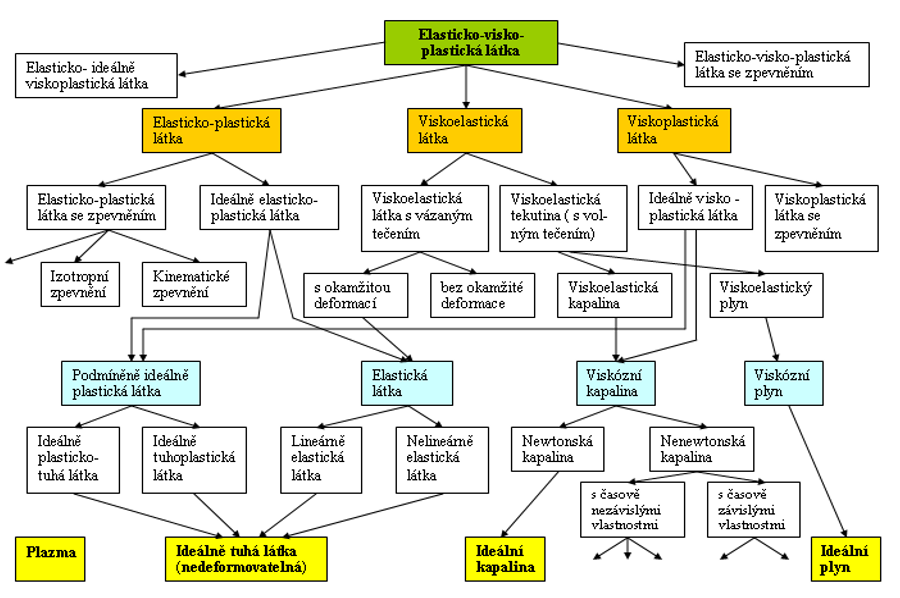
\includegraphics[width=0.7\linewidth]{prehled-konstitutivnich-modelu}
	\caption{Přehled konstitutivních modelů}
	\label{fig:prehled-konstitutivnich-modelu}
\end{figure}

% !TeX root = skripta-konstitutivni-vztahy.tex
% !TeX lastmodified = 2018-10-02

\subsection{Přechod k~integrálnímu popisu viskoelastické látky}
Obecnější modely lze vytvořit rozšířením Kelvinova modelu.
\begin{figure}[H]
	\centering
	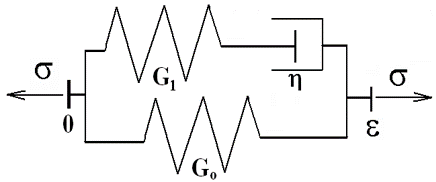
\includegraphics[width=0.4\linewidth]{standard-linear-solid}
	\caption{Standard linear solid}%todo změnit
\end{figure}

Jeho relaxace napětí je popsána rovnicí
\begin{equation}
	\sigma(t) = \varepsilon_0 \left[G_0 + G_1 \exp\! \left(-\frac{t}{\tau_\varepsilon} \right) \right] = \varepsilon_0 K(t),
\end{equation}
kde $K(t)$ je tzv. relaxační funkce.

Přidáváním dalších paralelních Maxwellových elementů do celkového počtu $n$ ji lze zobecnit do tvaru
\begin{equation}
	K(t) = \sum\limits_{i=0}^n G_i \exp\! \left(-\frac{t}{\tau_\varepsilon} \right) = \sum\limits_{i=0}^n G_i \exp\! \left(-t \nu_i\right),
\end{equation}
kde $\nu_i = \frac{1}{\tau_i}$ je relaxační frekvence $i$-tého Maxwellova prvku.

Vynesením závislosti amplitud $G_i$ jako funkce těchto frekvencí dostaneme diskrétní spektrum relaxačních funkcí.

\subsubsection{Diskrétní spektrum relaxačních funkcí}
Amplitudy jednotlivých členů $\alpha_i$ jsou zde normalizovány vůči celkovému modulu podle vztahu
\begin{equation}
	\alpha_i = \frac{G_i}{\sum_{i=0}^n G_i}
\end{equation}

\begin{figure}[H]
	\centering
	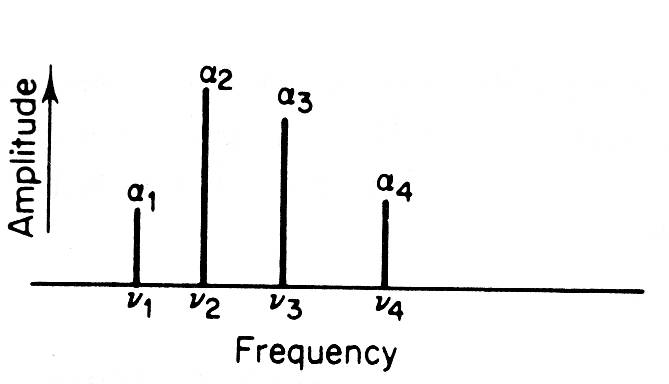
\includegraphics[width=0.4\linewidth]{spektrum-relaxacnich-funkci}
	\caption{Diskrétní spektrum relaxačních funkcí}
	\label{fig:spektrum-relaxacnich-funkci}
\end{figure}

\subsubsection{Boltzmannova formulace}
Nejobecnější formulace Boltzmannova vychází z~těchto předpokladů:
\begin{itemize}
	\item deformace je funkcí celé historie zatěžování až do vyšetřovaného času $t$,
	\item existuje proporcionalita (lineární závislost) mezi přírůstkem napětí $\diff \sigma(t)$ a~přírůstkem deformace $\diff \varepsilon(t)$,
	\item funkce $\sigma(t)$ je spojitá a~diferencovatelná.
\end{itemize}

Pak přírůstek napětí v~krátkém časovém intervalu $\diff \tau$ v~časovém okamžiku $\tau$ je $\left(\frac{\partial \sigma}{\partial \tau}\right) \diff \tau$.
Tento přírůstek napětí působí na těleso po celý zbývající časový interval $(t - \tau)$ a~k~přetvoření v~čase~$t$ přispívá přírůstkem $\diff \varepsilon(t)$, jehož závislost na přírůstku napětí v~čase je popsána funkcí $K$. Ta závisí na příslušném časovém intervalu $(t - \tau)$, takže platí
\begin{equation}
	\diff \varepsilon(t) = K(t - \tau) \frac{\partial \sigma}{\partial \tau} \diff \tau,
\end{equation}
kde funkce $K(t - \tau)$ je označována jako krípová nebo retardační funkce, resp. také relaxační funkce přetvoření.
Pokud položíme časový počátek do počátku pohybu (zatěžování), tak přetvoření lze určit integrací
\begin{equation}
	\varepsilon(t) = \int\limits_0^t K(t - \tau) \frac{\partial \sigma}{\partial \tau} \diff \tau.
\end{equation}

\subsubsection{Konvoluční integrál relaxační funkce}
Zaměníme-li roli napětí a~přetvoření (deformační zatěžování), pak dostaneme stejným postupem podobnou formulaci pro napětí:
\begin{equation}
	\sigma(t) = \int\limits_0^t C(t - \tau) \frac{\partial \varepsilon}{\partial \tau} \diff \tau,
\end{equation}
kde funkce $C(t - \tau)$ je relaxační funkce napětí. Zobrazení této funkce v~závislosti na čase nebo frekvenci představuje spojité relaxační spektrum.

Při začátku zatěžování v~čase $t = -\infty$, za předpokladu malých přetvoření i~posuvů, lze popsat závislost mezi napětími a~přetvořeními rozšířenými na tenzorové funkce závislé kromě času i~na prostorových souřadnicích bodu $\bm{x}(x_1, x_2, x_3)$ konvolučním integrálem 
\begin{equation}
	\sigma_{ij}(\bm{x}, t) = \int\limits_{-\infty}^t G_{ijkl}(\bm{x}, t - \tau) \frac{\partial \varepsilon_{kl}}{\partial \tau} (\bm{x}, \tau) \diff \tau,
\end{equation}
nebo jeho inverzním tvarem
\begin{equation}
	\varepsilon_{ij}(\bm{x}, t) = \int\limits_{-\infty}^t J_{ijkl}(\bm{x}, t - \tau) \frac{\partial \sigma_{kl}}{\partial \tau} (\bm{x}, \tau) \diff \tau,
\end{equation}
kde $G_{ijkl}$ je tenzorová relaxační funkce a~$J_{ijkl}$ je tenzorová krípová funkce.

V~praxi nelze integrovat od času $t = -\infty$, volíme tedy počátek časové osy v~okamžiku počátku pohybu, kdy těleso bylo nezatížené a~nedeformované.
Pak je např. konvoluční integrál pro napětí zredukován do tvaru
\begin{equation}
	\sigma_{ij}(\bm{x}, t) = \varepsilon_{kl}(\bm{x}, 0\!+) G_{ijkl}(\bm{x}, t)
	+ \int\limits_0^t G_{ijkl}(\bm{x}, t - \tau) \frac{\partial \varepsilon_{kl}}{\partial \tau} (\bm{x}, \tau) \diff \tau,
\end{equation}
kde $\varepsilon_{kl}(\bm{x}, 0+)$ je limita funkce $\varepsilon_{kl}(\bm{x}, t)$ pro $t \rightarrow 0$ zprava.
První člen na pravé straně rovnice představuje důsledek skokové změny přetvoření v~čase $t = 0$; podobný člen je třeba zavést v~každém časovém okamžiku, kdy funkce $\varepsilon_{kl}(\bm{x}, t)$ nemá derivaci (skokově se mění).

Zpracováno podle Funga\footnote{Y.C. Fung: Biomechanics. Springer, 1993.}.

\section{Alternativní vyjádření podmínky plasticity}
% !TeX root = skripta-konstitutivni-vztahy.tex
% !TeX lastmodified = 2018-12-10

\subsection{Misesova mezní podmínka energetická formulace}
Ekvivalentní napětí podle von Misese je v~kurzu PP na FSI v Brně odvozováno jako podmínka plasticity (HMH), založená na velikosti oktaedrického smykového napětí.
Ke stejné podmínce lze však dospět i~na základě energetického přístupu, kdy mezní stav (plasticity nebo pevnosti, podmínka je používána i~jako pevnostní kriterium) nastane tehdy, když měrná deformační energie změny tvaru (deviátorová) dosáhne jisté mezní hodnoty, která je materiálovou charakteristikou.
Ve velkých deformacích je ekvivalentní napětí skalární hodnotou Cauchyho tenzoru (skutečného) napětí.

V~jednoosé napjatosti je měrná deformační energie
\begin{equation}
	w_e = \frac{\diff W_e}{\diff V} = \int\limits_0^\varepsilon \sigma \diff \varepsilon
\end{equation}
a~pro lineárně elastický materiál se dá zjednodušit do tvaru
\begin{equation}
	w_e = \frac{1}{2} \sigma \varepsilon = \frac{\sigma^2}{2 E} = \frac{1}{2} E \varepsilon^2
\end{equation}

Pro víceosou napjatost je třeba do deformační energie zahrnout příspěvek všech složek tenzorů napětí a~přetvoření. Přitom složky s~nestejnými indexy spolu svírají pravý úhel, takže jejich příspěvek k~deformační práci je nulový.

Měrnou energii lze tedy zapsat ve tvaru:
\begin{equation}\begin{split}
	w_e
	= &\int\limits_{0}^{\varepsilon_{11}} \sigma_{11} \diff \varepsilon_{11}
	+ \int\limits_{0}^{\varepsilon_{12}} \sigma_{12} \diff \varepsilon_{12}
	+ \int\limits_{0}^{\varepsilon_{13}} \sigma_{13} \diff \varepsilon_{13}
	+ \int\limits_{0}^{\varepsilon_{21}} \sigma_{21} \diff \varepsilon_{21}\\
	+ &\int\limits_{0}^{\varepsilon_{22}} \sigma_{22} \diff \varepsilon_{22}
	+ \int\limits_{0}^{\varepsilon_{23}} \sigma_{23} \diff \varepsilon_{23}
	+ \int\limits_{0}^{\varepsilon_{31}} \sigma_{31} \diff \varepsilon_{31}
	+ \int\limits_{0}^{\varepsilon_{32}} \sigma_{32} \diff \varepsilon_{32}
	+ \int\limits_{0}^{\varepsilon_{33}} \sigma_{33} \diff \varepsilon_{33}
\end{split}\end{equation}

Tenzorovým zápisem lze zjednodušit do tvaru
\begin{equation}
	w_e
	= \int\limits_{0}^{\bm{\varepsilon}} \bm{\sigma} \!:\! \bm{\varepsilon} 
	\:\Leftrightarrow\: \int\limits_{0}^{\varepsilon_{ij}} \sigma_{ij} \diff \varepsilon_{ij},
\end{equation}
kde $\bm{\sigma}$ a~$\bm{\varepsilon}$ jsou tenzory druhého řádu a~v~indexovém zápisu platí Einsteinovo sčítací pravidlo.

Použijeme-li ve vztahu rozklad tenzorů napětí a~deformace na jejich kulové a~deviátorové složky, dostaneme měrnou energii napjatosti následovně:
\begin{equation}\begin{split}%todo už nepoužíváme index e?
	w
	= &\int\limits_0^{\bm{\varepsilon}} \left(\bm{\sigma}' + \frac{\mathrm{Sp}(\bm{\sigma})}{3}\bm{1}\right)
	\!:\! \left(\diff \bm{\varepsilon}' + \frac{\mathrm{Sp}(\diff \bm{\varepsilon})}{3}\bm{1}\right)\\
	= &\int\limits_0^{\bm{\varepsilon}'} \bm{\sigma}' \!:\! \diff \bm{\varepsilon}'
	+ \int\limits_0^{\bm{\varepsilon}} \left( \frac{\mathrm{Sp}(\bm{\sigma})}{3}\bm{1} \right) \!:\! \left( \frac{\mathrm{Sp}(\diff \bm{\varepsilon})}{3}\bm{1} \right)
	= w_d + w_V,
\end{split}\end{equation}
kde čárka v~horním indexu značí deviátorovou složku tenzoru.

Měrná energie napjatosti tedy sestává z~části deviátorové $w_d$ (energie změny tvaru) a~objemové $w_V$ (energie změny objemu).

Misesova podmínka vychází z deviátorové části energie napjatosti $w_d$ (dané změnou tvaru), kterou lze tedy zapsat následovně:
\begin{equation}
	w_d = \int\limits_0^{\bm{\varepsilon}'} \bm{\sigma}' \!:\! \diff \bm{\varepsilon}' \:\Leftrightarrow\: \int\limits_0^{\varepsilon'_{ij}} \sigma'_{ij} \diff \varepsilon'_{ij}
\end{equation}

Použijeme-li pro lineárně elastický materiál Hookeův zákon s~oddělenou tvarovou a~objemovou složkou, platí:
\begin{equation}
	\sigma_{ij}
	= 2 G \varepsilon_{ij} + \lambda \varepsilon_{ii}
	= 2 G \varepsilon'_{ij} + K \varepsilon_{ii}
\end{equation}
a~tedy pro deviátorové složky napětí a~přetvoření
\begin{equation}
	\sigma'_{ij} = 2 G \varepsilon'_{ij}
\end{equation}
nebo inverzní tvar pro hodnotu nebo přírůstek deviátoru deformace
\begin{equation}
	\varepsilon'_{ij} = \frac{\sigma'_{ij}}{2 G} \qquad
	\diff\varepsilon'_{ij} = \frac{\diff \sigma'_{ij}}{2 G}
\end{equation}
Pak lze měrnou energii tvarové změny vyjádřit pomocí pouze napětí anebo pomocí přetvoření následovně:
\begin{equation}
	w_d
	= \int\limits_0^{\varepsilon'_{ij}} \sigma'_{ij} \diff \varepsilon'_{ij}
	= \frac{1}{2} \sigma'_{ij} \varepsilon'_{ij}
	= \frac{1}{4 G} \sigma'_{ij} \sigma'_{ij}
	= G \varepsilon'_{ij} \varepsilon'_{ij}
	= G \bm{\varepsilon}' \!:\! \bm{\varepsilon}'
\end{equation}

Zavede-li se redukované napětí vztahem
\begin{equation}
	\sigma_\text{ekv}^2
	= \frac{3}{2} (\bm{\sigma}' \!:\! \bm{\sigma}')
	\:\Leftrightarrow\: \sigma_{ij}' \sigma_{ij}',
\end{equation}
pak lze deviátorovou část energie napjatosti $w_d$ zapsat následovně:
\begin{equation}
	w_d = \frac{\sigma_\text{ekv}^2}{6 G}.
\end{equation}

Zavede-li se podobně redukované přetvoření podle Misesovy podmínky, lze energii vyjádřit také s~jeho použitím
\begin{equation}
	w_d
	= \frac{2}{3} G (1+\mu)^2 \varepsilon_\text{ekv}^2
	= \frac{E (1+\mu)}{3} \varepsilon_\text{ekv}^2.
\end{equation}

\subsubsection{Misesova mezní podmínka jako izotropní zjednodušení podmínky Tsai-Hill pro kompozity}
Misesova energetická podmínka je obecně používána i~jako podmínka pevnosti u~technických i~biologických materiálů.
Nejsnadněji lze shodu obou přístupů ukázat pomocí energetické podmínky Tsai-Hill uváděné\footnote{Agarval, Broutman: Vláknové kompozity. SNTL Praha, 1987} pro vláknové kompozity ve tvaru
\begin{equation}
	\left(\frac{\sigma_L}{\sigma_{PL}}\right)^2
	- \frac{\sigma_L}{\sigma_{PL}} \frac{\sigma_T}{\sigma_{PT}}
	+ \left(\frac{\sigma_T}{\sigma_{PT}}\right)^2
	+ \left(\frac{\tau_{LT}}{\tau_P}\right)^2 < 1,
\end{equation}
kde indexy $L$, $T$ označují hlavní směry materiálu a~index $P$ pevnost v~daném směru.

Po zjednodušení na materiál izotropní ($\sigma_{PL}= \sigma_{PT} = \sigma_P$) a~zavedení pevnosti ve smyku podle Misesovy podmínky ve tvaru
\begin{equation}
	\tau_P = \frac{\sigma_P}{\sqrt{3}},
\end{equation}
převedeme výše uvedenou nerovnici na tvar
\begin{equation}
	\left(\frac{\sigma_L}{\sigma_{PL}}\right)^2
	- \frac{\sigma_L \sigma_P}{\sigma_P^2}
	+ \left(\frac{\sigma_T}{\sigma_P}\right)^2
	+ \left(\frac{\sqrt{3} \tau_{LT}}{\sigma_P}\right)^2 < 1.
\end{equation}

Výsledný tvar podmínky (platný pro rovinnou napjatost) pak je
\begin{equation}\label{tsai-hill-kompozit}
	\sqrt{\sigma_L^2 - \sigma_L\sigma_T + \sigma_T^2 + 3\tau_{LT}^2} < \sigma_P.
\end{equation}

Redukované (ekvivalentní) napětí podle Misesovy podmínky (HMH) se pro obecný souřadnicový systém obvykle uvádí ve tvaru\footnote{Janíček, Ondráček Vrbka, Burša: Mechanika těles -- Pružnost a pevnost I. CERM Brno, 2006.}
\begin{equation}
	\sigma_\text{red}
	= \sqrt{\frac{1}{2} \bigg[ (\sigma_L-\sigma_T)^2 + (\sigma_L-\sigma_{T'})^2 + (\sigma_T-\sigma_{T'})^2 + 6 \left( \tau_{LT}^2 + \tau_{LT'}^2 + \tau_{TT'}^2 \right) \bigg]},
\end{equation}
kde označení os $x$, $y$, $z$ bylo pouze změněno na $L$, $T$, $T'$.
Pro dvouosou napjatost v~rovině $LT$ pak dostáváme tvar
\begin{equation}
	\sigma_\text{red} = \sqrt{\sigma_L^2 - \sigma_L\sigma_T + \sigma_T^2 + 3\tau_{LT}^2},
\end{equation}
z~nějž porovnáním s~rovnicí (\ref{tsai-hill-kompozit}) plyne obvyklý tvar mezní podmínky
\begin{equation}
	\sigma_\text{red} < \sigma_P,
\end{equation}
který se od obvyklé Misesovy podmínky plasticity liší jen použitou mezní hodnotou.

% !TeX root = skripta-konstitutivni-vztahy.tex
% !TeX lastmodified = 2018-12-11

\subsection{Misesova mezní podmínka vyjádřená pomocí přetvoření}
Mezní podmínku podle von Misese lze odvodit také energetickým přístupem, kdy mezní stav (plasticity nebo pevnosti, podmínka je používána i~jako pevnostní kriterium) nastane tehdy, když měrná deformační energie změny tvaru (deviátorová) dosáhne jisté mezní hodnoty, která je materiálovou charakteristikou.

Tuto energii napjatosti lze pak vyjádřit duálně pomocí napětí nebo přetvoření.
Vyjádříme-li ji pomocí přetvoření, dospějeme k~pojmu redukované (ekvivalentní) přetvoření, což je největší hlavní přetvoření při jednoosé napjatosti (tj. přetvoření ve směru působícího zatížení), které dává podle Misesovy podmínky stejnou bezpečnost vůči meznímu stavu jako vyšetřovaný víceosý deformačně-napěťový stav. 

Pro deviátorové složky přetvoření a~napětí platí obecný vztah
\begin{equation}
	\bm{\sigma}' = 2 G \bm{\varepsilon}',
\end{equation}
zatímco pro ekvivalentní jednoosou napjatost
\begin{equation}
	\sigma_\text{ekv} = E \varepsilon_\text{ekv} = 2 G (1+\mu) \varepsilon_\text{ekv},
\end{equation}
takže člen $1+\mu$ se musí objevit v~redukovaném přetvoření.

\subsubsection{Misesova mezní podmínka pro ekvivalentní (redukované) přetvoření}
Ekvivalentní přetvoření je definováno vztahem
\begin{equation}
	\varepsilon_\text{ekv} = \frac{1}{1+\mu} \sqrt{\frac{1}{2} \left[ (\varepsilon_x-\varepsilon_y)^2 + (\varepsilon_x-\varepsilon_z)^2 + (\varepsilon_y-\varepsilon_z)^2 + \frac{6}{4} \left( \gamma_{xy}^2 + \gamma_{xz}^2 + \gamma_{yz}^2 \right) \right]}.
\end{equation}
Pro oceli v~plastické oblasti je Poissonovo číslo $\mu=\num{0.5}$, takže platí
\begin{equation}
	\varepsilon_\text{ekv} = \frac{2}{3} \sqrt{\frac{1}{2} \left[ (\varepsilon_x-\varepsilon_y)^2 + (\varepsilon_x-\varepsilon_z)^2 + (\varepsilon_y-\varepsilon_z)^2 + \frac{6}{4} \left( \gamma_{xy}^2 + \gamma_{xz}^2 + \gamma_{yz}^2 \right) \right]},
\end{equation}
případně ve 2D (rovinná deformace)
\begin{equation}
	\varepsilon_\text{ekv} = \frac{2}{3} \sqrt{ \varepsilon_x^2 - \varepsilon_x\varepsilon_y + \varepsilon_y^2 + \frac{3}{4} \gamma_{xy}^2 }.
\end{equation}


\section{Tekutiny}
% !TeX root = skripta-konstitutivni-vztahy.tex
% !TeX lastmodified = 2006-09-11

\subsection{Stavová rovnice ideálního plynu}
se obvykle zapisuje ve tvaru
\begin{equation}
	p v = r T,
\end{equation}
kde
\begin{description}
	\item[$p$] je tlak plynu,
	\item[$v$] je měrný objem plynu,
	\item[$r$] je měrná plynová konstanta,
	\item[$T$] je absolutní teplota.
\end{description}

Vynásobíme-li uvedenou rovnici molovou hmotností látky $M$, změní se na levé straně měrný objem plynu na molový objem plynu a~na pravé straně se změní měrná plynová konstanta na univerzální (molovou) plynovou konstantu $R_m$, jejíž hodnota je pro všechny ideální plyny stejná a~činí $R_m = \SI{8.3143 \pm 0.0012}{\joule\per\mole\per\kelvin}$.

Známý $p-V$ diagram izotermického (tj. hyperbola), resp. adiabatického (strmější adiabata) děje lze znázornit v~souřadnicích střední napětí $\sigma_s$ -- poměrná změna objemu $e$
\begin{figure}[H]
	\centering
	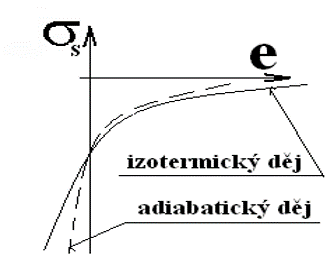
\includegraphics[height=4cm]{izotermicky-adiabaticky-dej}
	\caption{$\sigma_s-e$ diagram}
	\label{fig:izotermicky-adiabaticky-dej}
\end{figure}

% !TeX root = skripta-konstitutivni-vztahy.tex
% !TeX lastmodified = 2006-09-01

\subsection{Co je ideální plyn?}
Charakteristické vlastnosti ideálního plynu:
\begin{itemize}
	\item Nulová viskozita, tj. žádné vnitřní tření, nulový odpor proti změně tvaru -- shodné s~ideální kapalinou.
	\item Značná objemová stlačitelnost, a současně rozpínavost, tj. schopnost vyplnit celý disponibilní prostor. Odpor proti změně objemu je velmi malý a~řídí se stavovou rovnicí ideálního plynu.
\end{itemize}

% !TeX root = skripta-konstitutivni-vztahy.tex
% !TeX lastmodified = 2006-09-01

\subsection{Co je ideální kapalina?}
Charakteristické vlastnosti ideální kapaliny:
\begin{itemize}
	\item Nulová viskozita, tj. žádné vnitřní tření, nulový odpor proti změně tvaru.
	\item Objemová nestlačitelnost, tj. nekonečně velký odpor proti změně objemu.
\end{itemize}

% !TeX root = skripta-konstitutivni-vztahy.tex
% !TeX lastmodified = 2006-09-01

\subsubsection{Tvar tenzoru napětí pro ideální kapalinu}
\begin{itemize}
	\item Všechna normálová napětí záporná a~stejně velká -- důsledek Pascalova zákona
	\item Smyková napětí nulová -- důsledek nulové viskozity
\end{itemize}

\begin{equation}
	\bm{\sigma} = \left(\begin{matrix}
		-p &  0 &  0\\
		 0 & -p &  0\\
		 0 &  0 & -p\\
	\end{matrix}\right)
\end{equation}

\chapter{Modely elastického chování}
\subsection{Úvod}
% !TeX root = skripta-konstitutivni-vztahy.tex
% !TeX lastmodified = 2006-09-11

\section{Co je to elasticita?}
Elasticita je schopnost látky vrátit se po zatížení a~odlehčení do původního tvaru.
Podle tvaru deformačně-napěťové charakteristiky dělíme tyto látky na lineárně a~nelineárně elastické.

Charakteristiky:
\begin{figure}[H]
	\label{fig:linearne-elasticka-latka}
	\centering
	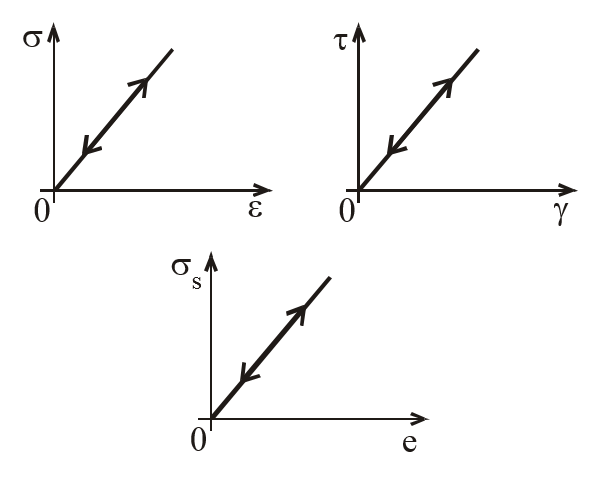
\includegraphics[width=0.7\linewidth]{linearne-elasticka-latka}
	\caption{lineárně elastické látky}
\end{figure}

\begin{figure}[H]
	\label{fig:nelinearne-elasticka-latka}
	\centering
	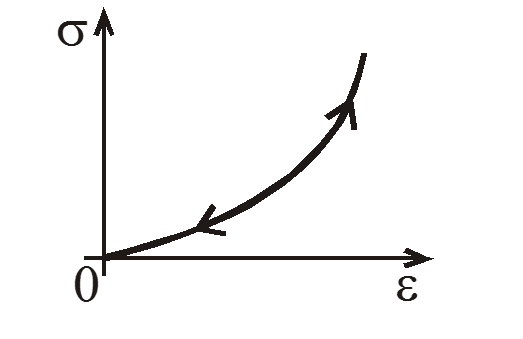
\includegraphics[width=0.7\linewidth]{nelinearne-elasticka-latka}
	\caption{nelineárně elastické látky}
\end{figure}

% !TeX root = skripta-konstitutivni-vztahy.tex
% !TeX lastmodified = 2016-12-14

\subsection{Upravený tvar Hookova zákona}\label{sec:hookeuv-zakon}
Vztahy vyjadřující vzájemnou závislost elastických konstant izotropního hookovského materiálu
\begin{align}
G &= \frac{E}{2 (1+\mu)}\\
K &= \frac{E}{3 (1 - 2\mu)}\\
\lambda &= \frac{E \mu}{(1 + \mu)(1 - 2\mu)} = K - \frac{2}{3} G
\end{align}

Vyjdeme ze tvaru s~explicitně vyjádřenými napětími (viz PPII)
\begin{equation}\begin{split}
\sigma_1
&= 2 G \varepsilon_1 + \lambda (\varepsilon_1 + \varepsilon_2 + \varepsilon_3) =
2 G \varepsilon_1 + \left(K - \frac{2}{3} G\right)\left(\varepsilon_1 + \varepsilon_2 + \varepsilon_3\right)\\
&= 2 G \left(\varepsilon_1 - \frac{\varepsilon_1 + \varepsilon_2 + \varepsilon_3}{3}\right) + K \left(\varepsilon_1 + \varepsilon_2 + \varepsilon_3\right) =
2 G D_{\varepsilon_1} + K e
\end{split}\end{equation}

\subsection{Hookův zákon v tenzorovém tvaru}
Složkové rovnice Hookova zákona
\begin{align}
\sigma_1 &= 2 G D_{\varepsilon_1} + K e\\
\sigma_2 &= 2 G D_{\varepsilon_2} + K e\\
\sigma_3 &= 2 G D_{\varepsilon_3} + K e\\
\tau_{12} &= G \gamma_{12} = 2 G D_{\varepsilon_{12}}\\
\tau_{23} &= G \gamma_{23} = 2 G D_{\varepsilon_{23}}\\
\tau_{31} &= G \gamma_{13} = 2 G D_{\varepsilon_{13}}
\end{align}%todo opravit zápis

Deviátor tenzoru přetvoření
\begin{equation}
D_\varepsilon = \left( \begin{matrix}
\varepsilon_1 - \varepsilon_s & \frac{\gamma_{12}}{2} & \frac{\gamma_{13}}{2}\\
\frac{\gamma_{21}}{2} & \varepsilon_2 - \varepsilon_s & \frac{\gamma_{23}}{2}\\
\frac{\gamma_{13}}{2} & \frac{\gamma_{23}}{2} & \varepsilon_3 - \varepsilon_s
\end{matrix} \right)
\end{equation}

Obecný zápis Hookova zákona
\begin{equation}
\sigma_{ij} = 2 G D_{s_{ij}} + \delta_{ij} K e
\end{equation}
kde $\delta_{ij}$ je Kroneckerův symbol.
\begin{equation}
\delta_{ij} = 1 \forall i = j \quad a \quad \delta_{ij} = 0 \forall i \neq j
\end{equation}

Analogický zápis Newtonova zákona
\begin{equation}
\sigma_{ij} = 2 \eta \dot{D}_{s_{ij}} + \delta_{ij} \kappa \dot{e}
\end{equation}
kde $\kappa\:[Pa.s]$ je objemová („druhá“) viskozita
% !TeX root = skripta-konstitutivni-vztahy.tex
% !TeX lastmodified = 2016-02-10

\subsection{Závislost elastických konstant}
Vztahy pro modul pružnosti ve smyku a~Lamého konstantu $\lambda$ byly odvozeny v~PPII přímo ve tvarech
\begin{align}
	G &= \frac{E}{2(1+\mu)}\\
	\lambda &= \frac{E \mu}{(1+\mu) (1-2\mu)}
\end{align}

Modul objemové pružnosti je definován podobně jako v~hydromechanice
\begin{equation}
	K = \frac{\sigma_s}{e},
\end{equation}
kde
\begin{itemize}
	\item[$\sigma_s$] je střední napětí,
	\item[$e$] je poměrná změna objemu.
\end{itemize}

Pro tyto veličiny byly v~PPII odvozeny vztahy
\begin{align}
	\sigma_s &= \frac{\sigma_1 + \sigma_2 + \sigma_3}{3},\\
	e &= \varepsilon_1 + \varepsilon_2 + \varepsilon_3,
\end{align}
do nichž dosadíme z Hookova zákona a~dostaneme:
\begin{equation}\begin{split}
	e
	&= \varepsilon_1 + \varepsilon_2 + \varepsilon_3
	= \frac{1}{E} \left[\sigma_1 - \mu(\sigma_2 + \sigma_3)\right]
	+ \frac{1}{E} \left[\sigma_2 - \mu(\sigma_1 + \sigma_3)\right]
	+ \frac{1}{E} \left[\sigma_3 - \mu(\sigma_1 + \sigma_2)\right]\\
	&= \frac{1}{E} \left[\sigma_1 (1-2\mu) + \sigma_2 (1-2\mu) + \sigma_3 (1-2\mu)\right]
	= \frac{1-2\mu}{E} \left(\sigma_1 + \sigma_2 + \sigma_3\right)
\end{split}\end{equation}

Dosazením do definičního vztahu pro $K$ dostaneme
\begin{equation}
	K
	= \frac{\sigma_s}{e}
	= \frac{\frac{\sigma_1 + \sigma_2 + \sigma_3}{3}}{\frac{(1-2\mu) (\sigma_1 + \sigma_2 + \sigma_3)}{E}}
	= \frac{E}{3 (1-2\mu)}
\end{equation}

Hookův zákon potřebujeme vyjádřit pomocí konstant, které mají analogii v~hydromechanice, tedy pomocí $K$ a~$G$.
Tak vyjádříme i~Lamého konstantu $\lambda$
\begin{equation}
	\lambda
	= \frac{E \mu}{(1+\mu) (1-2\mu)} \frac{3}{3}
	= \frac{E(1+\mu) - E(1-2\mu)}{3 (1+\mu) (1-2\mu)}
	= \frac{E}{3(1-2\mu)} - \frac{E}{3(1+\mu)} \frac{2}{2}.
	= K - \frac{2}{3} G
\end{equation}

Obráceně, pokud známe $K$ a~$G$, tedy moduly pro objemovou a~deviátorovou část deformace, můžeme dopočítat Poissonovo číslo $\mu$ (které dává obvyklou představu o~stlačitelnosti materiálu) ze vztahu
\begin{equation}
	\mu = \frac{3K - 2G}{6K + 2G}.
\end{equation}

% !TeX root = skripta-konstitutivni-vztahy.tex
% !TeX lastmodified = 2018-11-20

\subsection{Entropická elasticita}
Při teplotě absolutní nuly jakékoli vlákno (řetězec, makromolekula) zaujímá tvar minimalizující jeho energii, což odpovídá přímému prutu, pokud rozhodující veličinou je celková deformační energie včetně energie vynaložené na ohybovou deformaci vlákna $W_\text{bend}$
\begin{equation}
	W_\text{bend} = \left(\frac{K_f}{2}\right) \int\limits_0^L \left(\frac{\partial t}{\partial s}\right)^2 \diff s,
\end{equation}
kde
\begin{description}
	\item[$K_f = EJ$] je ohybová tuhost vlákna,
	\item[$\diff s$] element délky vlákna (křivočarý),
	\item[$L$] (contour length) je celková křivočará délka vlákna (rovná vzdálenosti jeho konců v napřímeném tvaru),
	\item[$\tfrac{\partial t}{\partial s}$] je rychlost změny tečného vektoru podél délky~$s$ vlákna (lokální křivost).
\end{description}

\begin{figure}[H]
	\centering
	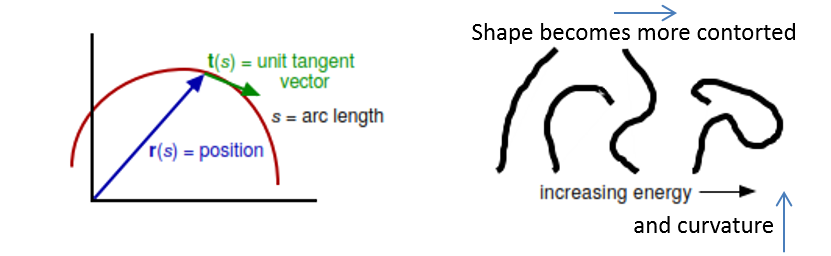
\includegraphics{entropicka-elasticita}
	\caption{Entropická elasticita}
	\label{fig:entropicka-elasticita}
\end{figure}

\subsubsection{Entropie}
Entropie $S$ je mírou pravděpodobnosti daného stavu; v~termodynamice vratných dějů je definována následovně:
\begin{equation}
	\diff S := \frac{\diff Q}{T}
\end{equation}

Pro makromolekulární řetězec je entropie definována pomocí maximálního počtu dosažitelných (tvarových) konfigurací:
\begin{equation}
	S := \ln\left(\text{maximální počet možných konfigurací}\right)
\end{equation}

S~rostoucí entropií určitého tvaru tedy roste pravděpodobnost, že se tento tvar řetězce reálně vyskytne.
Pak pravděpodobnost $P(E)$, že vlákno s~určitou energií $W_\text{bend}$ se vyskytne právě v~určité specifické konfiguraci (tvaru), lze vyjádřit vztahem
\begin{equation}
	P(E) = \exp\left(-\frac{W_\text{bend}}{k_B T}\right),
\end{equation}
kde pravá strana vyjadřuje Boltzmannův faktor\footnote{Fung, YC, 1993}\footnote{Boal, MC, 2002}.

S~rostoucí entropií určitého tvaru roste pravděpodobnost, že se tento tvar řetězce reálně vyskytne.
Pro látky s~nezanedbatelným vlivem entropie na elastické chování není rozhodující veličinou samotná deformační energie, ale Gibbsova volná energie.

\subsubsection{Gibbsova a~Helmholtzova volná energie $G$}
je největší množství energie uchované v soustavě za izotermických a~izobarických (Gibbsova) nebo izovolumických (Helmholtzova) podmínek.

\begin{itemize}
	\item Gibbsova volná energie -- Termodynamika plynů a~par (konstantní tlak)
	\begin{equation}
	\Delta G = \Delta H - T \Delta S,
	\end{equation}
	\item Gibbsova volná energie -- Obecný tvar pro všechna skupenství
	\begin{equation}
	\Delta G = \Delta E + p \Delta V - T \Delta S,
	\end{equation}
	\item Helmholtzova volná energie -- Tvar platný pro tuhé skupenství (konstantní objem)
	\begin{equation}
	\Delta G = \Delta E - T \Delta S,
	\end{equation}
\end{itemize}
kde
\begin{description}
	\item[$H$] je entalpie,
	\item[$E$] je vnitřní  energie,
	\item[$T$] je absolutní teplota,
	\item[$p$] je tlak,
	\item[$V$] je objem (pro látky v tuhém skupenství považován za konstantní)
\end{description}

Pro izotermický děj odpovídá minimalizace volné energie spontánnímu procesu, tj. $\Delta G < 0$ s~nárůstem entropie.
Je-li však vlákno natahováno, klesá počet možných konfigurací (na jedinou v~plně napřímené konfiguraci), tedy klesá i~entropie, což odpovídá procesu nespontánnímu, tj. $\Delta G > 0$.
\footnote{[2] Boal, MC, 2002; [3] Sean, E, 2010; [6] Mofrad , CM, 2006; [15] Mucke, JMB, 2004}

\subsubsection{Perzistentní délka -- délka stálosti tvaru}
Při nenulové absolutní teplotě $T$ dochází k~ohybu přímé tyče vlivem výměny energie s~okolím (u~molekul Brownův pohyb).
Perzistentní délka (persistence length) $L_p$ určuje délku, pod níž se (molekulární) řetězec chová jako tyč s +významnou ohybovou tuhostí, zatímco při délkách větších než $L_p$ se chová jako ohebné vlákno.
\begin{equation}
	L_p = \frac{K_f}{k_B T} = \frac{E J}{k_B T} = \frac{E}{k_B T} \left(\frac{\pi}{64} d^4\right),
\end{equation}
kde
\begin{itemize}
	\item[$E$] je Youngův modul,
	\item[$d$] je průměr vlákna,
	\item[$J$] je kvadratický moment.
\end{itemize}
Pak u~řetězce dochází k teplotním tvarovým fluktuacím; jeho tvar není jednoznačný, ale různé tvary jsou zaujímány s~různou pravděpodobností.

$L \ll L_p$ (tuhá tyč):
\begin{itemize}
	\item Řetězec se jeví přímý a~poměrně tuhý (prut).
	\item Pro jeho chování je rozhodující ohybová energie, bez vlivu entropie.
\end{itemize}

$L \gg L_p$ (ohebné vlákno) nebo $L \sim L_p$ (poloohebné vlákno):
\begin{itemize}
	\item Řetězec zaujímá spíše zakřivené tvary a~jeví se jako ohebné vlákno.
	\item Fluktuace tvaru a~následně energie v~termodynamické rovnováze se stávají významnými a~entropická elasticita se stává rozhodující (elastomery).
\end{itemize}

\subsubsection{Entalpická a~entropická elasticita}
Pro krystalické látky vnější zatížení mění rovnovážné meziatomární vzdálenosti a~zvyšuje vnitřní energii krystalu (entalpická elasticita).

Dlouhé ohebné molekuly elastomeru (gumy) jsou zakřivené a~tepelná energie je udržuje ve stálém termálním pohybu. Následně se s~deformací mění jejich entropie a~vzniká elastické napětí (entropická elasticita).

Z~porovnání entalpie, vnitřní energie a~volné energie plyne, že pokud je příspěvek entropické elasticity zanedbatelný, redukuje se uvedený přístup na entalpickou („klasickou“) elasticitu, obvyklou u~krystalických látek.
Pokud je příspěvek entropické elasticity dominantní (u~elastomerů), pak nárůst entropie (přirozený proces) odpovídá poklesu entalpie, resp. vnitřní energie (přirozený proces).

Entropická elasticita pocházející od protahování jednotlivých vláken termálními fluktuacemi se projevuje silnou nelinearitou.
Proto silné deformační zpevnění struktury je považováno za známku entropické elasticity.

\subsubsection{Entropická elasticita u~jednovláknového polymeru}
Při nulové teplotě $L_p \gg L$
\begin{figure}[H]
	\centering
	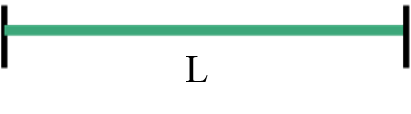
\includegraphics[height=2cm]{jednovlaknovy-polymer-nulova-teplota}
	\caption{Jednovláknový kompozit při nulové teplotě}
	\label{fig:jednovlaknovy-polymer-nulova-teplota}
\end{figure}
Ohybová tuhost
\begin{equation}
	K_f = L_p K_B T
\end{equation}

Při nenulové teplotě $L_p \ll L$
\begin{figure}[H]
	\centering
	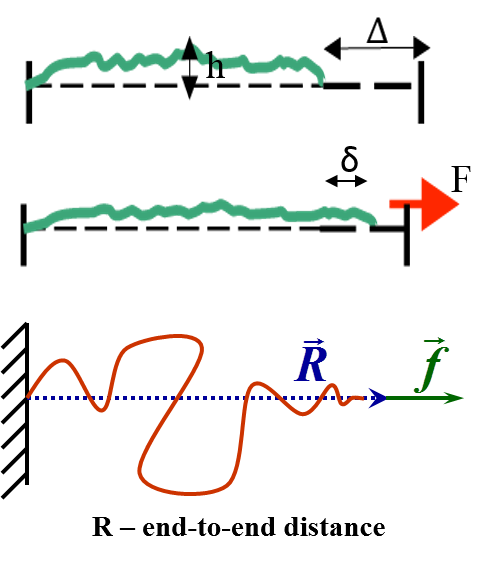
\includegraphics{jednovlaknovy-polymer-nenulova-teplota}
	\caption{Jednovláknový kompozit při nenulové teplotě}
	\label{fig:jednovlaknovy-polymer-nenulova-teplota}
\end{figure}

Síla $f$ se rovná derivaci Gibbsovy volné energie podle $R$
\footnote{[2] Boal, Mechanics of the Cell, 2002; [17] Bustamante, Science, 1994}
\begin{equation}
	f = \frac{\delta G}{\delta R} = \frac{3 K_B T R}{L_p L}
\end{equation}

\subsubsection{Původ elasticity pro různé materiály}
\begin{figure}[H]
	\centering
	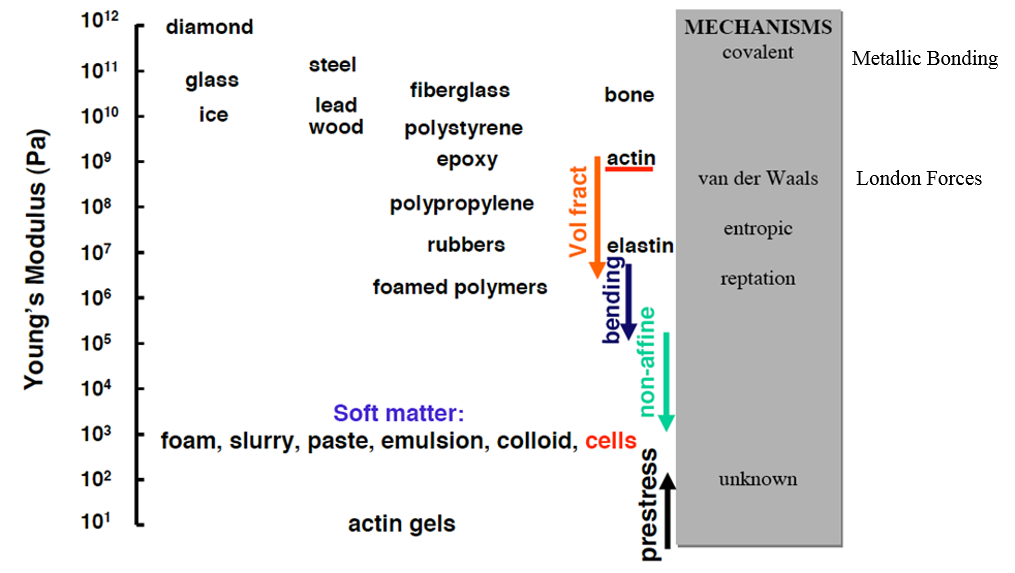
\includegraphics[width=0.7\linewidth]{elasticita-materialu}
	\caption{Elasticita různých materiálů}
	\label{fig:elasticita-materialu}
\end{figure}

Pro krystalické látky vnější zatížení mění rovnovážné meziatomární vzdálenosti a~zvyšuje vnitřní energii krystalu (entalpická elasticita).

Dlouhé ohebné molekuly gumy jsou zakřivené a~tepelná energie je udržuje ve stálém termálním pohybu.
Následně se s deformací mění jejich entropie a~vzniká elastické napětí (entropická elasticita).\footnote{[1] Fung ,B, 1993; [2] Boal , MC, 2002; [6] Mofrad , CM, 2006; [24] Fabry, CGM, 2003}

% !TeX root = skripta-konstitutivni-vztahy-materialu.tex
% !TeX lastmodified = 2019-11-06

\section{Hyperelasticita -- Konstitutivní vztahy elastomerů}

Jako hyperelastické označujeme materiály vykazující konečná vratná přetvoření.

Konečná přetvoření jsou taková která nejsou infinitezimální tedy nekonečně malá.
V~praxi jsou to přetvoření větší než cca \SI{1}{\percent}, chyba vzniklá jejich zanedbáním však roste nelineárně a~stává se velmi významnou, dosáhnou-li přetvoření desítek procent. 

\subsection{Rozdíly oproti teorii malých deformací}

Definice délkových přetvoření pro malé deformace
\begin{equation}\label{pretvoreni_male_deformace}
	\varepsilon_x = \frac{\partial u}{\partial X}
	\qquad
	\varepsilon_y = \frac{\partial v}{\partial Y}
	\qquad
	\varepsilon_z = \frac{\partial w}{\partial Z}
\end{equation}

Definice normálových napětí pro malá přetvoření
\begin{equation}\label{napeti_male_deformace}
	\sigma_x = \frac{\partial F_x}{\partial Y \partial Z}
	\qquad
	\sigma_y = \frac{\partial F_y}{\partial X \partial Z}
	\qquad
	\sigma_z = \frac{\partial F_z}{\partial X \partial Y}
\end{equation}

Obě veličiny jsou vztaženy k~původním (nedeformovaným) rozměrům elementu (obrázek).
\begin{figure}[H]
	\centering
	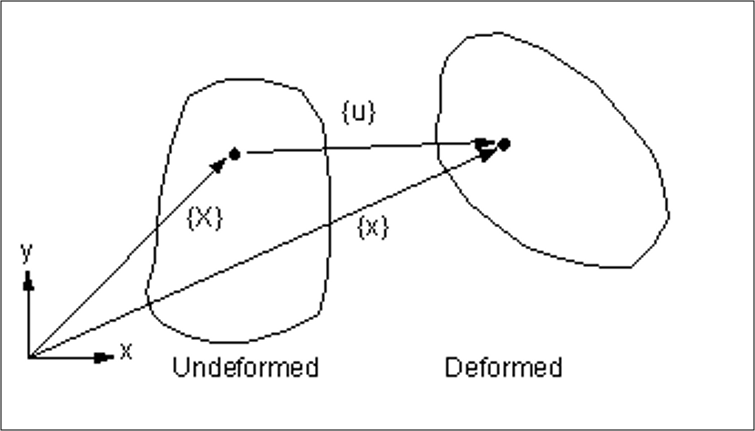
\includegraphics[height=3cm]{deformovane-nedeformovane-souradnice}
	\caption{Rozměry elementu}
\end{figure}

U~velkých deformací jsou však skutečné (deformované) rozměry podstatně odlišné od původních a~to je třeba respektovat.
Proto jsou zavedeny různé definice tenzorů přetvoření i~napětí.

\subsection{Tenzory popisující stav deformace v~bodě tělesa}
\begin{itemize}
	\item Pro malé deformace -- smluvní přetvoření (engineering strain)
	\item Green-Lagrangeův tenzor přetvoření
	\item Almansiho-Hamelův tenzor přetvoření
	\item Cauchyho (logaritmický) tenzor přetvoření
	\item Tenzor deformačního gradientu
	\item Cauchy-Greenův tenzor deformace (pravý a~levý)
	\item Tenzor protažení (stretch tensor)
\end{itemize}

Pro praktické použití jsou důležité vztahy pro vzájemný převod jednotlivých tenzorů přetvoření.

\subsection{Tenzory popisující napjatost v~bodě tělesa}
\begin{itemize}
	\item Piola-Kirchhoffův tenzor napětí 1.~druhu
	\item Cauchyho tenzor napětí (skutečná napětí -- true stress)
	\item Piola-Kirchhoffův tenzor napětí 2.~druhu
\end{itemize}

Pro správné (jednoznačné) určení energie napjatosti je nutné pracovat se vzájemně si odpovídajícími tenzory napětí a~přetvoření.
Těmto dvojicím tenzorů říkáme energeticky konjugované tenzory.
Takto konjugované jsou např.:
\begin{itemize}
	\item Green-Lagrangeův tenzor přetvoření a~2.~Piola-Kirchhoffův tenzor napětí,
	\item Pravý Cauchy-Greenův tenzor deformace a~2.~Piola-Kirchhoffův tenzor napětí,
	\item Pro praktické použití jsou důležité vztahy pro vzájemný převod jednotlivých tenzorů napětí.
\end{itemize}

\subsection{Vymezení hyperelastických materiálů}
Definice hyperelastického materiálu:
Materiál nazýváme hyperelastickým, pokud existuje elastická potenciální funkce $W$ (měrná deformační energie), která je skalární funkcí některého z~tenzorů přetvoření, resp. deformace a~jejíž parciální derivace podle některé složky přetvoření pak určuje odpovídající složku napětí.

To lze vyjádřit např. následovně:
\begin{equation}
	S_{ij} = \frac{\partial W}{\partial E_{ij}} = 2 \frac{\partial W}{\partial C_{ij}},
\end{equation}
kde
\begin{description}
	\item[$S_{ij}$] jsou složky 2.~Piola-Kirchhoffova tenzoru napětí
	\item[$W$] je funkce měrné energie napjatosti na jednotku nedeformovaného objemu
	\item[$E_{ij}$] jsou složky Green-Lagrangeova tenzoru přetvoření
	\item[$C_{ij}$] jsou složky pravého Cauchy-Greenova deformačního tenzoru
\end{description}

Kontrolní otázka: Vyhovuje této definici hyperelasticity hookovský materiál? Odpověď.
%todo zde prezentace energie-otazka-ppt

\subsection{Výpočet Cauchyho napětí u~hyperelastických materiálů}
Přepočet mezi tenzory napětí lze vyjádřit následovně:
\begin{equation}\label{key}
\sigma_{ij} = \frac{\rho}{\rho_0} F_{iR} S_{RS} F_{jS},
\end{equation}
kde
\begin{description}
	\item[$S_{RS}$] jsou složky 2.~Piola-Kirchhoffova tenzoru napětí,
	\item[$\sigma_{ij}$] jsou složky Cauchyho tenzoru (skutečného) napětí.
\end{description}

Napětí vypočítané parciální derivací je 2.~Piola-Kirchhoffovo, vynásobením  složkou tenzoru deformačního gradientu dostaneme postupně 1.~Piola-Kirchhoffovo a~Cauchyho napětí (odpovídá přepočtu mezi tenzory napětí).
Tak dostaneme vztah platný pro nestlačitelný materiál.
Protože však je měrná energie napjatosti $W$ vztažena na jednotku objemu v~nedeformovaném stavu, pro stlačitelný materiál (objem se mění) je nutno výsledek vynásobit poměrem měrných hmotností, kde $\rho_0$ odpovídá nedeformovanému a~$\rho$ deformovanému stavu.

\subsection{Rozdělení deformace na objemovou a~tvarovou složku}
U~všech hyperelastických konstitutivních modelů je stejně jako u~většiny ostatních třeba odděleně modelovat objemovou a~tvarovou (deviátorovou) složku deformace.
Proto konstitutivní vztahy sestávají ze dvou částí:
\begin{itemize}
	\item Vliv změny objemu na energii napjatosti popisují nejčastěji třetím invariantem tenzoru gradientu deformace $J$ a~konstantou popisující objemovou změnu (objemový modul pružnosti nebo jiná konstanta z~něj odvozená). Kromě pěnových gum je změna objemu malá oproti změně tvaru a~většinou vystačíme s~jejím lineárním popisem.
	\item Vliv tvarové změny se popisuje nejčastěji pomocí modifikovaných invariantů některého z tenzorů přetvoření. Modifikace má za cíl právě oddělení tvarové změny (deviátorové složky tenzoru) od změny objemové (kulová složka tenzoru).
\end{itemize}

\subsection{Přehled konstitutivních modelů respektujících velká přetvoření}
\subsubsection{Modely (hyper)elastické}
Izotropní (téměř) nestlačitelné: 
\begin{itemize}
	\item \hyperref[sec:neo-hooke]{Neo-Hooke}
	\item \hyperref[sec:mooney-rivlin]{Mooney-Rivlin}
	\item Klosner-Segal
	\item \hyperref[sec:yeoh]{Yeoh}
	\item \hyperref[sec:polynomicky-model]{Polynomial}
	\item Varga
	\item \hyperref[sec:model-ogden]{Ogden}
	\item Van der Waals
	\item \hyperref[sec:arruda-boyce]{Arruda-Boyce}
	\item Gent
	\item Pucci-Saccomandi
	\item Extended Tube
	\item Demiray
\end{itemize}

Izotropní stlačitelné
\begin{itemize}
	\item \hyperref[sec:ogden-foam]{Ogden (foam)}
	\item \hyperref[sec:blatz-ko]{Blatz-Ko (foam)}
	\item Hill-Storakers (foam)
\end{itemize}

\hyperref[sec:anizotropni-hyperelasticke-modely]{Anizotropní (téměř) nestlačitelné}
\begin{itemize}
	\item \hyperref[sec:polynomicky-anizotropni-hyperelasticky-model]{Polynomický}
	\item Fung
	\item Choi-Vito
	\item \hyperref[sec:model-hgo]{Holzapfel, 2000}
	\item Holzapfel, 2005
	\item Gasser (rozptyl směrů vláken, zjednodušená integrace)
	\item Microfiber (rozptyl směrů vláken, plná integrace)
\end{itemize}

\subsubsection{Modely neelastického chování}
Modely s~Mullinsovým efektem
\begin{itemize}
	\item \hyperref[sec:ogden-roxburgh]{Ogden-Roxburgh}
	\item Kachanov
	\item Miehe
	\item Marckmann
\end{itemize}

Visko-hyperelastické modely
\begin{itemize}
	\item \hyperref[sec:bergstrom-boyce]{Bergström-Boyce}
\end{itemize}

Elasto-plastické modely
\begin{itemize}
	\item \hyperref[sec:ramberg-osgood]{Ramberg-Osgood}
	\item \hyperref[sec:chaboche]{Chaboche}
\end{itemize}

Creepové modely
\begin{itemize}
	\item \hyperref[sec:norton]{Norton}
\end{itemize}

\subsubsection{Model Neo-Hooke}
Tento model zavádí měrnou energii napjatosti ve tvaru\footnote{(Treloar, 1975, pro nestlačitelnost odvozen termodynamicky již 1934)}
\begin{equation}\label{neo_hooke}
	W = \frac{G}{2} \left( \bar{I}_1 - 3 \right) + \frac{1}{d} \left( J - 1 \right)^2,
\end{equation}
kde
\begin{description}
	\item[$G$] je počáteční modul pružnosti ve smyku, přičemž platí $G = 2nkT$, kde $n$ je počet molekulárních řetězců v~jednotkovém objemu, $k$~je Boltzmanova konstanta a~$T$ je absolutní teplota,
	\item[$\bar{I}_1$] je modifikovaný první invariant pravého Cauchy-Greenova tenzoru deformace,
	\item[$d$] je parametr stlačitelnosti materiálu, daný vztahem $d = \frac{2}{K}$, kde $K$ je objemový modul pružnosti,
	\item[$J$] je třetí invariant tenzoru deformačního gradientu.
\end{description}

Vzhledem k~tomu, že tvarová změna je u~tohoto modelu popsána jedinou elastickou konstantou, je tento model použitelný do cca \SI{30}{\percent}, kdy nelinearita není příliš výrazná. Model je lineární pro Cauchyho napětí a~levý Cauchy-Greenův deformační tenzor.

Platí $G = 2nkT$, kde $n$ je počet molekulárních řetězců v~jednotkovém objemu, $k$ je Boltzmanova konstanta a~$T$ absolutní teplota.

\subsubsection{Model Mooney-Rivlin 2-parametrický}
Tento model zavádí měrnou energii napjatosti ve tvaru
\begin{equation}
	W = c_{10} \left(\bar{I}_1 - 3\right) + c_{01} \left(\bar{I}_2 - 3\right) + \frac{1}{d} \left(J - 1\right)^2,
\end{equation}
kde
\begin{description}
	\item[$c10, c01$] jsou materiálové parametry,
	\item[$\bar{I}_1$] je modifikovaný první invariant pravého Cauchy-Greenova tenzoru deformace,
	\item[$\bar{I}_2$] je modifikovaný druhý invariant pravého Cauchy-Greenova tenzoru deformace,
	\item[$d$] je parametr stlačitelnosti materiálu, daný vztahem $d = \frac{2}{K}$, kde $K$ je objemový modul pružnosti,
	\item[$J$] je třetí invariant tenzoru deformačního gradientu.
\end{description}

Tento model je použitelný do cca \SI{100}{\percent} přetvoření, pokud křivka přetvoření-napětí nevykazuje inflexi.

\subsubsection{Model Mooney-Rivlin 5-parametrický}
Tento model zavádí měrnou energii napjatosti ve tvaru
\begin{equation}
	W
	= c_{10} \left(\bar{I}_1 - 3\right)
	+ c_{01} \left(\bar{I}_2 - 3\right)
	+ c_{20} \left(\bar{I}_1 - 3\right)^2
	+ c_{11} \left(\bar{I}_1 - 3\right) \left(\bar{I}_2 - 3\right)
	+ c_{02} \left(\bar{I}_2 - 3\right)^2
	+ \frac{1}{d} \left(J - 1\right)^2,
\end{equation}
kde
\begin{description}
	\item[$c10, c01, c_{20}, c_{11}, c_{02}$] jsou materiálové parametry,
	\item[$\bar{I}_1$] je modifikovaný první invariant pravého Cauchy-Greenova tenzoru deformace,
	\item[$\bar{I}_2$] je modifikovaný druhý invariant pravého Cauchy-Greenova tenzoru deformace,
	\item[$d$] je parametr stlačitelnosti materiálu, daný vztahem $d = \frac{2}{K}$, kde $K$ je objemový modul pružnosti,
	\item[$J$] je třetí invariant tenzoru deformačního gradientu.
\end{description}

Tento model je použitelný i~tehdy, když křivka přetvoření-napětí vykazuje inflexi.

\subsubsection{Model Mooney-Rivlin 9-parametrický}
Tento model zavádí měrnou energii napjatosti ve tvaru
\begin{multline}
W
= c_{10} \left(\bar{I}_1 - 3\right)
+ c_{01} \left(\bar{I}_2 - 3\right)
+ c_{20} \left(\bar{I}_1 - 3\right)^2
+ c_{11} \left(\bar{I}_1 - 3\right) \left(\bar{I}_2 - 3\right)
+ c_{02} \left(\bar{I}_2 - 3\right)^2\\
+ c_{30} \left(\bar{I}_1 - 3\right)^3
+ c_{21} \left(\bar{I}_1 - 3\right)^2 \left(\bar{I}_2 - 3\right)
+ c_{12} \left(\bar{I}_1 - 3\right) \left(\bar{I}_2 - 3\right)^2
+ c_{03} \left(\bar{I}_2 - 3\right)^3
+ \frac{1}{d} \left(J - 1\right)^2,
\end{multline}
kde
\begin{description}
	\item[$c10, c01, c_{20}, c_{11}, c_{02}, c_{30}, c_{21}, c_{12}, c_{03}$] jsou materiálové parametry,
	\item[$\bar{I}_1$] je modifikovaný první invariant pravého Cauchy-Greenova tenzoru deformace,
	\item[$\bar{I}_2$] je modifikovaný druhý invariant pravého Cauchy-Greenova tenzoru deformace,
	\item[$d$] je parametr stlačitelnosti materiálu, daný vztahem $d = \frac{2}{K}$, kde $K$ je objemový modul pružnosti,
	\item[$J$] je třetí invariant tenzoru deformačního gradientu.
\end{description}

Tento model je použitelný i~pro komplikované tvary křivek přetvoření-napětí.

\subsubsection{Model polynomický}\label{sec:polynomicky-model}
Tento model je zobecněním modelů Mooney-Rivlin.
Zavádí energii napjatosti ve tvaru
\begin{equation}
W
= \sum\limits_{i+j=1}^N c_{ij} \left(\bar{I}_1 - 3\right)^i \left(\bar{I}_2 - 3\right)^j
+ \sum\limits_{k=1}^M \frac{1}{d_k} \left(J - 1\right)^{2k},
\end{equation}
kde
\begin{description}
	\item[$c_{ij}$, $d_k$] jsou materiálové parametry,
	\item[$\bar{I}_1$] je modifikovaný první invariant pravého Cauchy-Greenova tenzoru deformace,
	\item[$\bar{I}_2$] je modifikovaný druhý invariant pravého Cauchy-Greenova tenzoru deformace,
	\item[$J$] je třetí invariant tenzoru deformačního gradientu.
\end{description}

Pro $M=1$ a $N= 1,2,3$ dostaneme jednotlivé modely Mooney-Rivlin.
U~těchto modelů je počáteční modul pružnosti ve smyku
\begin{equation}
	G = 2 \left(c_{10} + c_{01}\right).
\end{equation}
Pro počáteční objemový modul pružnosti zde platí vztah
\begin{equation}
	K = \frac{2}{d_1}.
\end{equation}

\subsubsection{Model Ogden}\label{sec:model-ogden}
Tento model zavádí energii napjatosti ve tvaru
\begin{equation}
	W
	= \sum\limits_{p=1}^N \frac{\mu_p}{\alpha_p} \left( \bar{\lambda}_1^{\alpha_p} + \bar{\lambda}_2^{\alpha_p} + \bar{\lambda}_3^{\alpha_p} - 3\right)
	+ \sum\limits_{p=1}^N \frac{1}{d_p} \left(J - 1\right)^{2p},
\end{equation}
kde
\begin{description}
	\item[$\mu_p, \alpha_p, d_p$] jsou materiálové parametry,
	\item[$\bar{\lambda}_i (i=1,2,3)$] jsou modifikovaná hlavní poměrná protažení, složky levého Cauchy-Greenova tenzoru deformace,
	\item[$J$] je třetí invariant tenzoru deformačního gradientu.
\end{description}

Pro $N = 1$ a~$\alpha_p = 2$ dostaneme model Neo-Hooke.

U~obecného Ogdenova modelu je počáteční modul pružnosti ve smyku
\begin{equation}
	G = \frac{1}{2} \sum\limits_{p=1}^1 \alpha_p \cdot \mu_p.
\end{equation}
Pro počáteční objemový modul pružnosti zde platí vztah
\begin{equation}
	K = \frac{2}{d_1}.
\end{equation}

Tento model dokáže popsat i~extrémně velké deformace.

\subsection{Zadávání vlastností hyperelastických materiálů v~programových systémech MKP}
Existují dvě základní možnosti zadávání vlastností hyperelastického materiálu do programových systémů MKP:
\begin{itemize}
	\item Pomocí zadání experimentálních závislostí napětí-přetvoření, z~nichž program vypočítá materiálové parametry zvoleného modelu. Volbu vhodného modelu provádíme obvykle na základě vizuálního porovnání experimentálních a~vypočtených křivek a~na základě vyčíslení celkové energetické chyby modelu.
	\item Pomocí přímého zadání elastických parametrů zvoleného modelu. Tento způsob lze použít:
	\begin{itemize}
		\item Při opakovaných výpočtech s materiálem, jehož konstanty jsme již dříve určili; vhodné jen při nepříliš odlišných deformačně-napěťových stavech.
		\item Pokud jsme konstanty modelu určili z~experimentů jiným způsobem. Základem výpočtu konstant je metoda nejmenších čtverců, která hledá hodnoty konstant při minimalizaci kvadrátů odchylek. Při samostatném určování materiálových parametrů je možné použít sofistikovanější metody jejich určování, např. relativní odchylky místo absolutních, zvýraznění nebo potlačení některých částí deformačně napěťových křivek pomocí váhových koeficientů nebo změnou počtu zadávaných bodů experimentálních křivek (viz \texttt{www.hyperfit.wz.cz}).
	\end{itemize}
\end{itemize}

\subsection{Vstupní údaje potřebné pro identifikaci konstant hyperelastických modelů}
Pro určení materiálových parametrů se používají následující typy zkoušek:
\begin{enumerate}
	\item Zkouška jednoosým tahem (v~jednoosé tahové napjatosti)
	\item Zkouška jednoosým tlakem (v~jednoosé tlakové napjatosti)
	\item Zkouška ekvibiaxiální (ve dvouosé rovnoměrné napjatosti)
	\item Zkouška smykem nebo krutem (ve smykové napjatosti)
	\item Zkouška tahem při nulových příčných posuvech (v~rovinné deformaci)
	\item Zkouška tlakem při nulových příčných posuvech (v~rovinné deformaci)
	\item Zkouška objemové stlačitelnosti (v~trojosé rovnoměrné napjatosti)
\end{enumerate}
Některé z~těchto zkoušek je v~praxi velmi obtížné realizovat (např. zkouška prostým smykem -- při velkých deformacích vznikají i~normálová napětí, zkouška krutem na tenkostěnné trubce pro vyvolání homogenní smykové napjatosti zase vede ke ztrátě tvarové stability).
Některé ze zkoušek jsou však pro nestlačitelný materiál vzájemně rovnocenné. Proto se v praxi provádějí jen některé z~nich.

Proč jsou nutné zkoušky ve víceosé napjatosti?

\subsection{Základní zkoušky pro identifikaci konstant hyperelastických modelů}
Pro určení materiálových parametrů hyperelastických konstitutivních modelů se v praxi nejčastěji používají následující základní typy zkoušek:
\begin{itemize}
	\item Zkouška jednoosým tahem (v~jednoosé tahové napjatosti). Realizuje se na běžných zkušebních strojích pro tahovou zkoušku na plochých normalizovaných vzorcích ve tvaru oboustranné lopatky.
	\item Zkouška ekvibiaxiální (ve dvouosé rovnoměrné napjatosti). Realizuje se na speciálních zkušebních strojích na plochých vzorcích kruhového nebo čtvercového tvaru.
	\item Zkouška tahem při nulových příčných posuvech (v~rovinné deformaci). Realizuje se na běžných zkušebních strojích pro tahovou zkoušku s~použitím velmi širokých čelistí na plochých vzorcích obdélníkového tvaru s~velmi malým poměrem délky ku šířce (cca 0,1).
	\item Zkouška objemové stlačitelnosti (v~trojosé rovnoměrné napjatosti). Realizuje se na běžných zkušebních strojích pro zkoušku tahem a tlakem na válcových vzorcích  (nejčastěji průměr $29mm$, výška cca $13mm$), vtlačovaných těsným pístem do ocelové komůrky stejného tvaru a~rozměrů.
\end{itemize}

\subsection{Zadávání výsledků zkoušky do programových systémů MKP}
Většina současných komerčních programových systémů MKP disponuje softwarem pro identifikaci materiálových parametrů jednotlivých hyperelastických modelů z naměřených experimentálních křivek napětí-přetvoření. Při jejich zadávání je třeba mít na paměti následující upozornění:
\begin{itemize}
	\item Rozsah zkoušek (extrémní velikost přetvoření) by měl mírně přesahovat očekávaný rozsah přetvoření v~řešeném výpočtovém modelu. Obvykle jej předem neznáme, jedná se tedy o~iterační proces, kdy v~prvním kroku zadáme raději maximální změřený rozsah přetvoření a~na základě výsledků jej poté upravujeme. Příliš velký rozsah modelu totiž významně snižuje jeho přesnost.
	\item Nemáme-li k~dispozici výsledky všech potřebných materiálových zkoušek, je velmi riskantní používání zdánlivě přesnějších modelů používajících např. polynomy vyšších stupňů. Dosáhneme tím sice přesnější aproximace zadaných křivek, ale výsledky pro jiné typy napjatosti mohou být zcela nesmyslné (nejsou podloženy experimentálními daty). Zásadně je možné takový výpočtový model použít jen pro řešení takových problémů, při nichž se nevyskytnou typy deformačně-napěťových stavů, pro něž nebyly zadány experimentální křivky. V~opačném případě mohou být výsledky zcela chybné, podobně jako když rozsah přetvoření při určitém typu napjatosti (např. při jednoosém tahu) přesáhne rozsah realizovaný při experimentu.
\end{itemize}

\subsection{Zásady pro práci s~hyperelastickými modely v~programových systémech MKP}
\begin{itemize}
	\item Vždy zevrubně prostudujeme manuál programu, abychom zjistili použitý tvar funkce pro energii napjatosti a~význam jednotlivých materiálových parametrů, což je důležité pro jejich správné použití a~orientační kontrolu jejich hodnot.
	\item Zjistíme, v~jakých tenzorech napětí a~přetvoření je třeba zadávat experimentální údaje.
	\item Zjistíme, v~jakých tenzorech napětí a~přetvoření obdržíme konečné výsledky. 
	\item Při každé práci s~novým konstitutivním modelem nebo novým programovým systémem vždy nejprve provedeme simulaci základních zadaných zkoušek materiálu, abychom na úloze se známými výsledky eliminovali chybný postup při tvorbě a~zadávání modelu.
\end{itemize}

% !TeX root = skripta-konstitutivni-vztahy-materialu.tex
% !TeX lastmodified = 2019-04-01

\subsection{Vyhovuje hookovský materiál definici hyperelastických materiálů?}
Funkce měrné energie napjatosti byla v~lineární PP odvozena např. pro jednoosou napjatost ve tvaru
\begin{equation}
	W = \frac{1}{2} \sigma_1:\varepsilon_1 = \frac{1}{2} \bm{\sigma}:\bm{\varepsilon}
\end{equation}
a~platí
\begin{equation}\label{eq:saint-venant-stress}
	\bm{S} = \frac{\partial W}{\partial \bm{E}}.
\end{equation}

Podle rovnice (\ref{eq:saint-venant-stress}) pak derivace energie napjatosti podle přetvoření (pro malé deformace libovolně definovaného, např. smluvního přetvoření $\varepsilon$) opravdu určuje odpovídající složku napětí (pro malé deformace opět podle libovolné definice tenzoru napětí), jak ukazuje následující výraz:
\begin{equation}
	S_{ij} = \frac{\partial W}{\partial E_{ij}}
	= \frac{\partial W}{\partial \varepsilon}
	= \frac{\partial \left(\frac{1}{2} \sigma \varepsilon\right)}{\partial \varepsilon}
	= \frac{\partial \left(\frac{1}{2} E \varepsilon^2\right)}{\partial \varepsilon}
	= \frac{2}{2} E \varepsilon = \sigma
\end{equation}
\textbf{Lineárně elastický materiál je tedy jen zvláštním případem materiálu hyperelastického.}
Podobně lze vyjádřit napětí i~pro víceosou napjatost.

\subsubsection{Energie napjatosti hookovského materiálu pro víceosou napjatost}
Funkci měrné energie napjatosti odvozenou v~lineární PP pro jednoosou a~smykovou napjatost lze zobecnit do tvaru
\begin{equation}
	W = \frac{1}{2} \sigma_{ij} \varepsilon_{ij}.
\end{equation}

Při rozepsání tohoto vztahu do složek je třeba vzít v~úvahu, že podle \hyperref[sec:einsteinovo-scitaci-pravidlo]{Einsteinova pravidla} jsou oba indexy $i$ a~$j$ sčítací.
Parciální derivace této energie napjatosti podle kterékoli složky přetvoření určuje odpovídající složku napětí.

% !TeX root = skripta-konstitutivni-vztahy.tex
% !TeX lastmodified = 2018-10-30

\subsection{Víceosé zkoušky elastomerů}
Neplatí princip superpozice a každá složka napětí je funkcí několika složek přetvoření.
Pro obecné vyjádření konstitutivních vlastností materiálu se proto používá měrná energie napjatosti, která je funkcí složek přetvoření.

\begin{figure}[H]
	\centering
	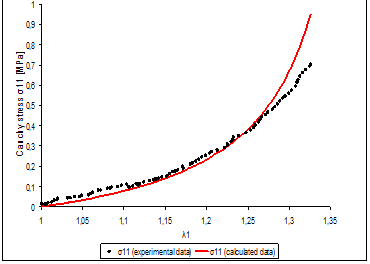
\includegraphics[height=4cm]{jednoosa-tahova-zkouska-tkane}
	\caption{Jednoosá tahová zkouška (měkké biologické tkáně)}
	\label{fig:jednoosa-tahova-zkouska-tkane}
\end{figure}

\begin{figure}[H]
	\centering
	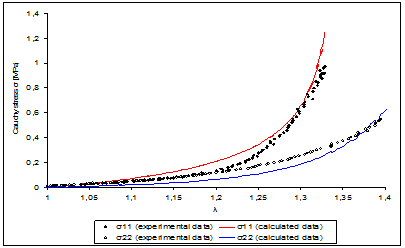
\includegraphics[height=4cm]{dvouosa-tahova-zkouska-tkane}
	\caption{Dvouosá tahová zkouška (měkké biologické tkáně)}
	\label{fig:dvouosa-tahova-zkouska-tkane}
\end{figure}

\subsubsection{Měrná energie napjatosti jako funkce dvou složek přetvoření}
Je tento materiál izotropní?
Jakým typům zkoušek odpovídají experimentální body vyznačené v~obrázku?
\begin{figure}[H]
	\centering
	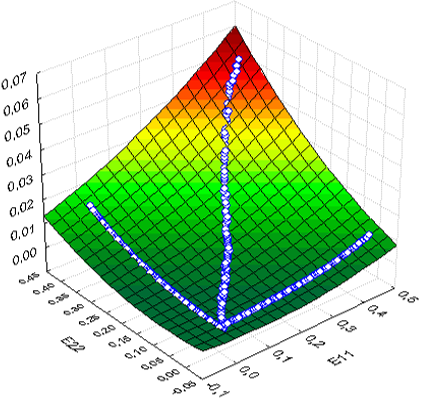
\includegraphics[height=4cm]{merna-energie-napjatosti}
	\caption{Měrná energie napjatosti}
	\label{fig:merna-energie-napjatosti}
\end{figure}

Použitá funkce pro energii napjatosti (Hayashi) má tvar:
\begin{equation}
	W = -C \ln(1-Q),
\end{equation}
kde
\begin{description}
	\item[{$Q = \frac{1}{2} c_1 E_{11}^2 + \frac{1}{2} c_2 E_{22}^2 + c_3 E_{11} E_{22}$}]
	\item[$E_{ii}$] jsou složky Green-Lagrangeova tenzoru přetvoření, 
	\item[{$C [\si{\pascal}]$}] je materiálový parametr definující tuhost materiálu,
	\item[$c_i$] jsou bezrozměrné materiálové parametry.
\end{description}

\subsubsection{Identifikace parametrů měrné energie napjatosti}
Pro identifikaci parametrů je definována funkce ve tvaru
\begin{equation}
	f_w = \sum\limits_{k=1}^n \left(\psi_k - W_k\right)^2,
\end{equation}
kde $\psi_k$ je deformační energie pro $k$-tý bod vypočítaná z~navrženého konstitutivního modelu
\begin{equation}
	\psi_k = \int\limits_0^{E^k_{11}} S_{11} \diff E_{11} + \int\limits_0^{E^k_{22}} S_{22} \diff E_{22}
\end{equation}
a~$W_k$ je deformační energie pro $k$-tý bod vypočítaná z~experimentálních dat pomocí rovnice
\begin{equation}
	W_k = \sum\limits_{j=1}^2 \sum\limits_{i=1}^k \frac{S_{jj}^i + S_{jj}^{i-1}}{2} \left(E_{jj}^i - E_{jj}^{i-1}\right)
\end{equation}

Pro konkrétní tvar konstitutivního modelu (např. logaritmickou funkci uvedenou na předchozí straně) se hledá taková kombinace jejích elastických parametrů, která minimalizuje funkci $f_w$ -- program Hyperfit\footnote{\texttt{http://hyperfit.wz.cz/}}.

\begin{figure}[H]
	\centering
	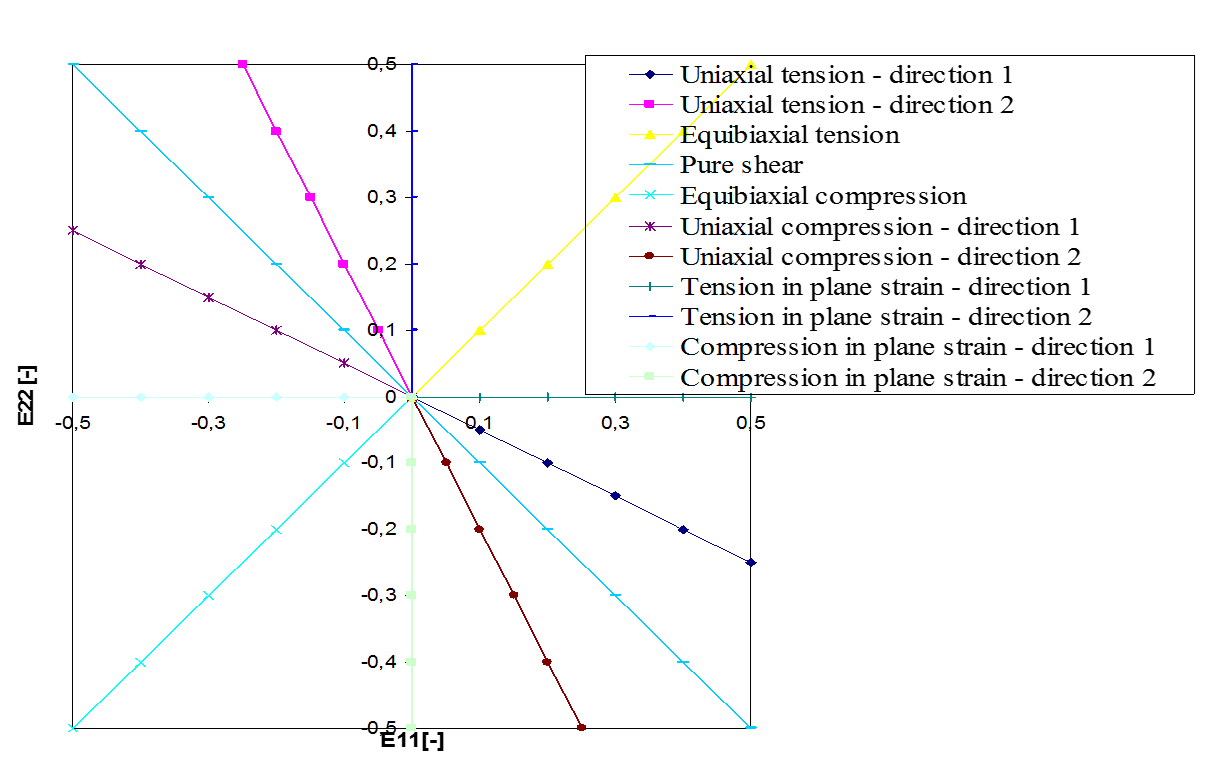
\includegraphics[width=0.6\linewidth]{zkousky-izotropniho-elastomeru}
	\caption[Zkoušky izotropního elastomeru]{Znázornění různých typů zkoušek izotropního elastomeru v~rovině dvou složek přetvoření}
	\label{fig:zkousky-izotropniho-elastomeru}
\end{figure}

\begin{figure}[H]
	\centering
	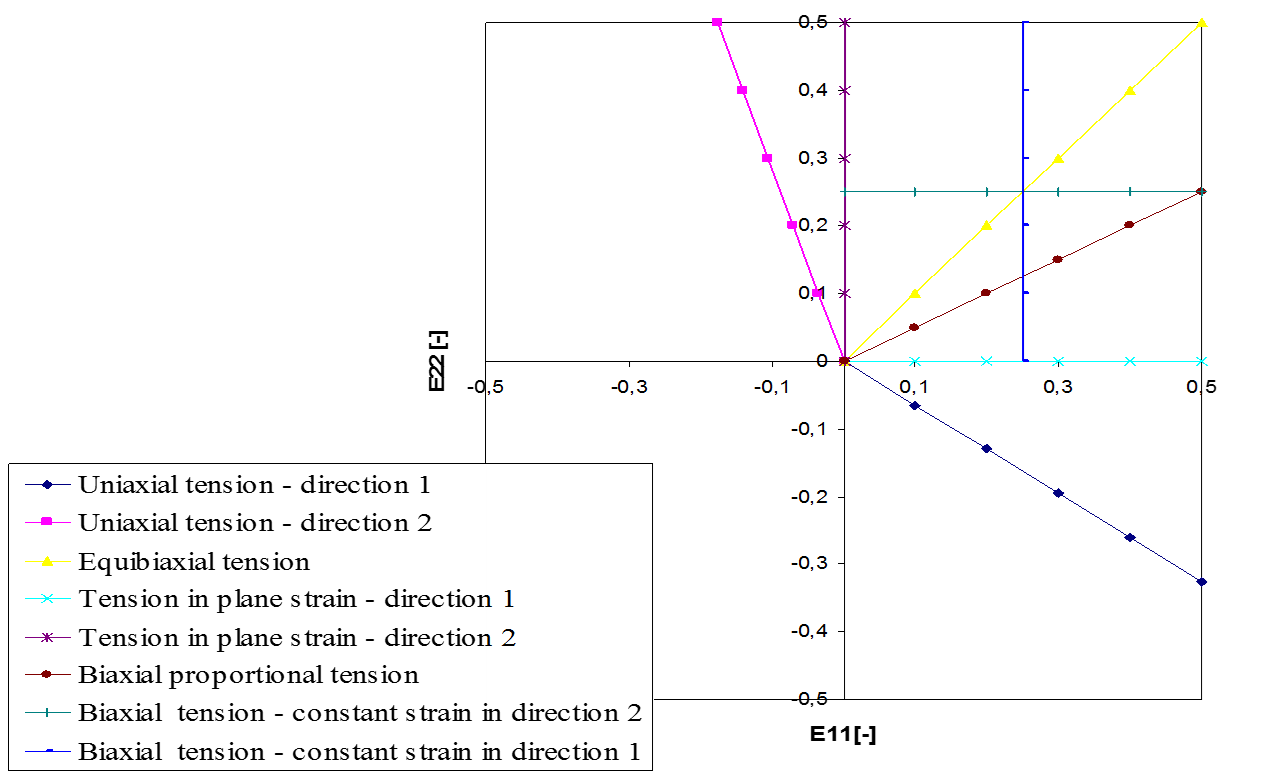
\includegraphics[width=0.6\linewidth]{zkousky-ortotropniho-elastomeru}
	\caption[Zkoušky ortotropního elastomeru]{Znázornění různých typů zkoušek ortotropního elastomeru v~rovině dvou složek přetvoření}
	\label{fig:zkousky-ortotropniho-elastomeru}
\end{figure}

Příklad konstitutivní rovnice ortotropního elastomeru
\begin{equation}
	W = c_1 E_{11}^2 + c_2 E_{11} E_{22} + c_3 E_{22}^2 + c_4 E_{11}^3 + c_5 E_{11}^2 E_{22} + c_6 E_{11} E_{22}^2 + c_7 E_{22}^3
\end{equation}

\begin{figure}[H]
	\centering
	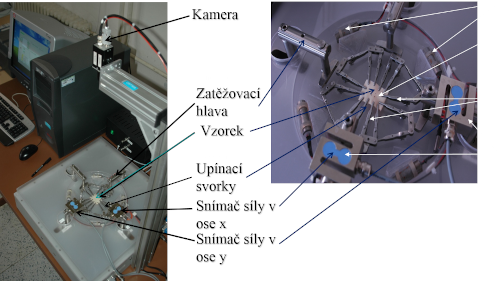
\includegraphics[width=0.7\linewidth]{zkusebni-stroj-elastomeru}
	\caption{Zkušební stroj pro zkoušky elastomerů ve dvouosé napjatosti}
	\label{fig:zkusebni-stroj-elastomeru}
\end{figure}

\section{Modely hyperelastického chování}
% !TeX root = skripta-konstitutivni-vztahy.tex
% !TeX lastmodified = 2016-11-01

\subsection{Model Neo-Hooke}\label{sec:neo-hooke}
\begin{itemize}
	\item NEO-HOOKE (1933-1934) 
	\item vědním oborem, který dal vznik tomuto modelu je „statistická mechanika“
	\item odvozen z představy o entropickém chování polymerních řetězců za předpokladu Gaussovského (normálního) rozdělení hustoty pravděpodobnosti poloh koncových bodů řetězců při jejich deformaci
	\item jedná se tak vlastně o první model, respektující strukturu materiálu (ať velmi elementárně, téměř nedokonale)
	\item Ve tvaru
\end{itemize}
\begin{equation}
	\psi = \frac{1}{2} G \left( \lambda_1^2 + \lambda_2^2 + \lambda_3^2 - 3 \right),
\end{equation}
přičemž
\begin{equation}
	G = N k T \sim \mu,
\end{equation}
kde
\begin{description}
	\item[$G$] je počet řetězců na jednotku objemu (počet částic daného množství)
	\item[$k$] je Boltzmanova konstanta $\SI{1.38064852e-23}{\joule\per\kelvin}$
	\item[$T$] he termodynamická teplota (zkrátka teplota)
	\item[$\mu$] je modul pružnosti ve smyku (u~nás značen $G = \frac{E}{2(1+\mu)}$, kde $\mu$ je Poissonovo číslo)
\end{description}

Také platí stavová rovnice ideálního plynu:
\begin{equation}
	p V = n R T = N k T \sim \mu
\end{equation}

Boltzmannova konstanta vyjadřuje vztah mezi teplotou a energií plynu. Vyjadřuje množství energie potřebné k zahřátí jedné částice ideálního plynu o jeden kelvin. Boltzmannova konstanta také úzce souvisí s entropií, protože stejně jako u entropie jde o množství energie na určitou teplotu. Byla pojmenována po rakouském fyzikovi Ludwigu Boltzmannovi, který se významně podílel na rozvoji statistické fyziky, kde tato konstanta hraje klíčovou roli.

Termodynamická teplota (též absolutní teplota nebo zkráceně teplota) je fyzikální stavová veličina dobře definovatelná protermodynamické systémy ve stavu termodynamické rovnováhy, rostoucí s růstem vnitřní energie systému. Její nerovnost určuje směr samovolného (tedy bez konání práce) přestupu tepla od teplejšího systému k systému chladnějšímu, uvedou-li se do tepelného kontaktu.

\subsubsection{Odvození}
Pro objasnění tvorby tohoto modelu je výhodně uvést i základní kroky vedoucí k jeho finální podobě

Základní předpoklady:
\begin{itemize}
	\item síť obsahuje obecně N řetězců na jednotku objemu
	\item žádná změna objemu během deformace (izochorický děj, nestlačitelný mat.)
	\item entropie sítě je dána součtem entropií jednotlivých řetězců
	\item koncové body mezi jednotlivými řetězci se při deformaci hýbou tak, jako by byly zality do elastického kontinua (afinní deformace)
\end{itemize}

\begin{figure}[H]
	\centering
	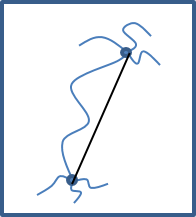
\includegraphics{Obrazky/sklon}
	\caption{Sklon pod úhlem $\alpha$}
	\label{fig:sklon}
\end{figure}
\begin{figure}[H]
	\centering
	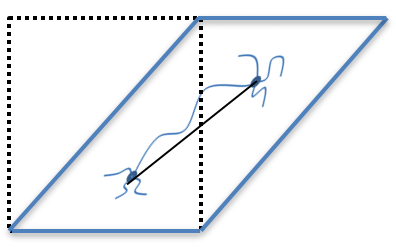
\includegraphics{Obrazky/sklon-rotace}
	\caption{Sklon pod úhlem $\alpha$ + rotace}
	\label{fig:sklon-rotace}
\end{figure}

Gaussovské rozdělení hustoty pravděpodobnosti poloh koncových bodů řetězce
\begin{figure}[H]
	\centering
	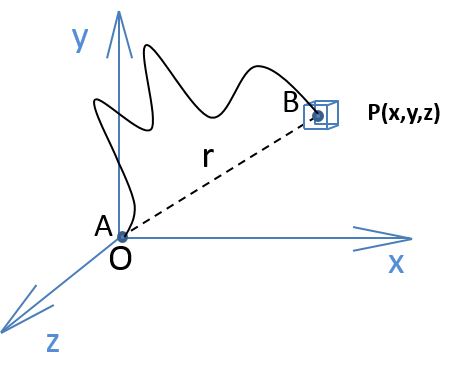
\includegraphics{Obrazky/kuhn}
	\caption{$P(x,y,z)$}
	\label{fig:kuhn}
\end{figure}
Kuhn (1934,1936) odvodil vztah, který reprezentuje pravděpodobnost, že složky vektoru $r$ definovaného spojnicí koncových bodů vlákna budou ležet v~intervalu:
\begin{equation}
od x do (x+dx)
od y do (y+dy)
od z do (z+dz)
\end{equation}
pravděpodobnost je
\begin{equation}
	p(x,y,z) \diff x \diff y \diff z
	= \frac{b^3}{\pi^{\frac{3}{2}}} \exp\left(-b^2(x^2 + y^2 + z^2)\right) \diff x \diff y \diff z
\end{equation}
přičemž
\begin{equation}
	b^2 = \frac{3}{2} n l^2
\end{equation}
a~uvažuje se $r << n l$
\begin{itemize}
	\item předpoklad, že vzdálenost není v~žádném případě srovnatelná s~nataženým řetězcem ($n l$)) 
	\item nezahrnuje také efekt postupného protažení (pak nutné použít ne-Gaussovské rozdělení)
\end{itemize}

Funkce je sféricky symetrická $x^2 + y^2 + z^2 = r^2$, proto
\begin{equation}
	p(x,y,z) \diff x \diff y \diff z
	= \frac{b^3}{\pi^{\frac{3}{2}}} \exp\left(-b^2(r^2)\right) \diff x \diff y \diff z
\end{equation}
pak zřejmě platí $p \rightarrow 1 \Leftrightarrow r \rightarrow 0$.

Distribuce spojnice koncových bodů vlákna -- distribuce $r$ vektoru (ne složek!!!)
\begin{figure}[H]
	\centering
	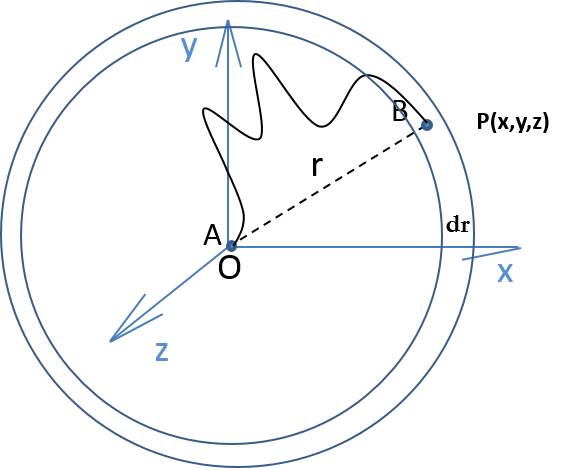
\includegraphics{Obrazky/distribuce-r}
	\caption{Distribuce $r$}
	\label{fig:distribuce-r}
\end{figure}

\begin{itemize}
	\item uvažujme všechny směry (x, y, z) stejně zastoupeny
	\item pak se bod B asi nepohybuje od x do x+dx, atd… ale je nutné aby se pohyboval např. po kulové skořepině s poloměrem r a elem. tloušťkou dr:
\end{itemize}
\begin{equation}
	P(r) \diff r
	= \frac{b^3}{\pi^{\frac{3}{2}}} \exp\left(-b^2(r^2)\right) 4 \pi r^2 \diff r
	= 4 \frac{b^3}{\pi^{\frac{1}{2}}} r^2 \exp\left(-b^2(r^2)\right) \diff r
\end{equation}
$P(r)$ je nulová při $r = 0$ a~dosahuje svého maxima ($r_m$) při: 
\begin{equation}
	\left(4 \frac{b^3}{\pi^{\frac{1}{2}}} r^2 \exp\left(-b^2 r^2\right)\right)
	= 0 \Rightarrow
	r_m = \frac{1}{b} = \sqrt{\frac{2 n l^2}{3}} \qquad\text{(příliš se však nepoužívá)}
\end{equation}
Důležitější je spíše hodnota střední hodnoty kvadrátu $r$, definovaná
\begin{equation}
	\bar{r^2} = \frac{\int_0^\infty r P(r) \diff r}{\int_0^\infty P(r) \diff r}
	= \frac{3}{2 b^2} = n l^2
\end{equation}

nyní se budeme snažit zjistit entropii jednoho řetězce a entropii soustavy řetězců (celé sítě). Začneme Boltzmanem (1887), který navrhl entropii (pro spojité izolované kontinuum) ve tvaru
\begin{equation}
	S = k \ln(\Omega),
\end{equation}
kde $\Omega$ charakterizuje část fázové prostoru (neboli počet rozlišitelných (mikro)stavů daného systému

Pravděpodobnostní prostor pohybu koncového bodu již máme definovaný
\begin{equation}
	\Omega = p(x,y,z) \diff \tau
	= \frac{b^3}{\pi^{\frac{3}{2}}} \exp\left(-b^2(r^2)\right) \diff \tau,
\end{equation}
tedy
\begin{equation}
	S
	= k \left\{\ln\left[p(x,y,z) \diff \tau\right]\right\}
	= k \left\{\ln\!\left(\frac{b^3}{\pi^{\frac{3}{2}}}\right) - b^2 r^2 + \ln(\diff \tau)\right\}
\end{equation}
z čehož vyplyne
\begin{equation}
	S = c - k b^2 r^2
\end{equation}

\begin{figure}[H]
	\centering
	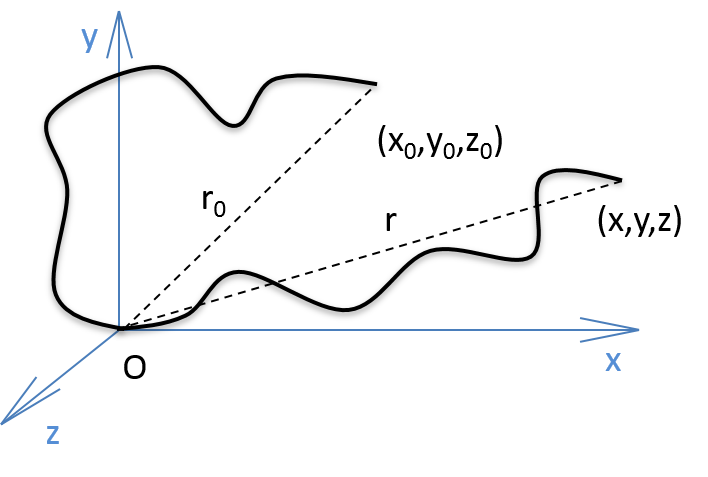
\includegraphics{Obrazky/neo-hooke-entropie}
	\caption{Řetězec}
	\label{fig:neo-hooke-entropie}
\end{figure}


\begin{itemize}
	\item entropie řetězce v~původním stavu:
	\begin{equation}
		S_0 = c - k b^2 r_0^2 = c - k b^2 (x_0^2 + y_0^2 + z_0^2)
	\end{equation}
	\item entropie řetězce v~deformovaném stavu
	\begin{equation}
		S = c - k b^2 r^2 = c - k b^2 (\lambda_1^2 x_0^2 + \lambda_2^2 y_0^2 + \lambda_3^2 z_0^2)
	\end{equation}
	\item příspěvek k~celkové entropii od tohoto jednoho řetězce
	\begin{equation}\begin{split}
		\Delta S &= S_0 - S
		= c - k b^2 (\lambda_1^2 x_0^2 + \lambda_2^2 y_0^2 + \lambda_3^2 z_0^2)
		- c + k b^2 (x_0^2 + y_0^2 + z_0^2)\\
		&= - k b^2 \left[ x_0^2(\lambda_1^2-1) + y_0^2(\lambda_2^2-1) + z_0^2(\lambda_3^2-1) \right]
	\end{split}\end{equation}
	\item Celková entropie sítě bude nejspíš součtem $N$ příspěvků $\Delta S$
	\begin{equation}
		S = \sum \Delta S = - k b^2 \left[ \sum x_0^2(\lambda_1^2-1) + \sum y_0^2(\lambda_2^2-1) + \sum z_0^2(\lambda_3^2-1) \right]
	\end{equation}
	$b$ je sice funkcí délky řetězce, nicméně pokud se předpokládá délka všech řetězců stejná, je $b$ konstantou
\end{itemize}

Protože jsou směry vektoru $r_o$ v~nezatíženém stavu zcela náhodné, nelze předpokládat žádnou preferenci směru $x$, $y$, nebo $z$. Tedy pravděpodobně platí
\begin{equation}
	\sum x_0^2 + \sum y_0^2 + \sum z_0^2 = \sum r_0^2
\end{equation}
a~zároveň
\begin{equation}
	\sum x_0^2 = \sum y_0^2 = \sum z_0^2 = \frac{1}{3} \sum r_0^2
\end{equation}
nicméně
\begin{equation}
	r_0^2 = N \bar{r_0^2},
\end{equation}
kde $\bar{r_0^2}$ je střední délka řetězců v~nedeformovaném stavu.

Po dosazení do celkové energie
\begin{equation}\begin{split}
	S &= \sum \Delta S
	= -\frac{1}{3} k N b^2 \bar{r_0^2} \left[ (\lambda_1^2-1) + (\lambda_2^2-1) + (\lambda_3^2-1) \right]\\
	&= -\frac{1}{3} k N b^2 \bar{r_0^2} \left( \lambda_1^2 + \lambda_2^2 + \lambda_3^2 - 3 \right)
\end{split}\end{equation}
kde
\begin{equation*}
	\bar{r_0^2} = \frac{3}{2} b^2
\end{equation*}
je entropie
\begin{equation}
	S = -\frac{1}{2} k N \left( \lambda_1^2 + \lambda_2^2 + \lambda_3^2 - 3 \right)
\end{equation}

Odvodili jsme entropii, ale potřebujeme energii \ldots otázkou tedy je, co dál?
Pomůže nám tzv. volná energie (Helmholtzova)
\begin{equation}
	\psi = U - TS
\end{equation}
Do které přispívají jak vnitřní energie (deformační energie přijata vychýlením se z~rovnovážných poloh daných vazbami krystalové mřížky), tak entropie (pocházející ze změny charakteru uspořádání). 

Ačkoliv se ani eleastomery nedeformuji čistě entropicky, příspěvek od vnitřní energie je často možné zanedbat proti příspěvku od změny entropie. 
\begin{equation}
	\psi = -TS = \frac{1}{2} k N T \left( \lambda_1^2 + \lambda_2^2 + \lambda_3^2 - 3 \right)
	= -\frac{1}{2} G \left( \lambda_1^2 + \lambda_2^2 + \lambda_3^2 - 3 \right)
\end{equation}

\subsubsection{Aplikace}
\begin{figure}[H]
	\centering
	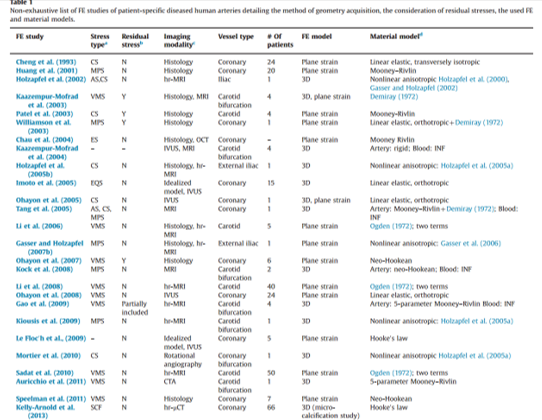
\includegraphics[width=0.7\linewidth]{Obrazky/neo-hooke-aplikace-1}
	\label{fig:neo-hooke-aplikace-1}
\end{figure}
\begin{figure}[H]
	\centering
	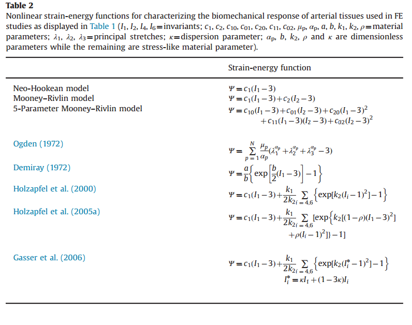
\includegraphics[width=0.7\linewidth]{Obrazky/neo-hooke-aplikace-2}
	\label{fig:neo-hooke-aplikace-2}
\end{figure}
\begin{figure}[H]
	\centering
	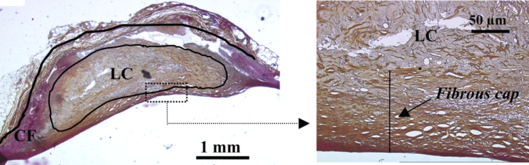
\includegraphics[width=0.7\linewidth]{Obrazky/neo-hooke-aplikace-3}
	\label{fig:neo-hooke-aplikace-3}
\end{figure}

\begin{align*}
	W = a (I_1 - 3)\\
	E_i \sim 6 a
\end{align*}

\begin{figure}[H]\centering\begin{tabular}{ll}\toprule
	Materiál & $E$\\ \midrule
	fibrosis & $\SI{500}{\kilo\pascal}$\\
	core & $\SI{5}{\kilo\pascal}$\\
	artery & $\SI{150}{\kilo\pascal}$\\
\bottomrule\end{tabular}\caption{Ohayon (2007)}\end{figure}

\subsubsection{Nenormální (neGaußovské) rozdělení pravděpodobnosti}
\begin{itemize}
	\item model Neo-Hook selhává při vyšších přetvořeních -- predikuje lineární odezvu, ač realita je silně nelineární
	\item důvodem je Gaussovské rozdělení pravděpodobnosti poloh koncových bodů vláken
	\item řešením je tedy použít ne-gaussovské rozdělení z čehož vznikají modely, jež bývají souhrnně označovány jako modely s~omezenou (někdy též limitovanou nebo konečnou) protažitelností řetězce -- limiting chain extensibility
	\item jedním z~nejznámějších je model \hyperref[sec:arruda-boyce]{Arruda-Boyce} (1998) nebo model Gent
\end{itemize}

% !TeX root = skripta-konstitutivni-vztahy.tex
% !TeX lastmodified = 2016-11-01

\subsection{Model Mooney-Rivlin}\label{sec:mooney-rivlin}
\subsubsection{Mooneyho formulace (1940)}\label{subsec:mooneyho-formulace}
\begin{itemize}
	\item guma je nestlačitelná a izotropní v nedeformovaném stavu
	\item Hookeův zákon platí pro „simple shear“ nebo „simple shear“ s~kombinací předchozího tlaku nebo tahu (simple shear v rovině kolmé na předchozí zatížení) 
\end{itemize}

Čistě matematická formulace hustoty deformační energie ve tvaru:
\begin{equation}
	W = C_1  \left(\lambda_1^2 + \lambda_2^2 + \lambda_3^2 - 3\right) + C_2 \left(\frac{1}{\lambda_1^2} + \frac{1}{\lambda_1^2} + \frac{1}{\lambda_1^2} - 3\right),
\end{equation}
kde $C_1 [\si{\mega\pascal}]$ a~$C_2 [\si{\mega\pascal}]$ jsou materiálové parametry.

Pokud $C_2 = 0$, pak existuje zřejmá podobnost s~modelem Neo-Hook
\begin{equation}
	2 C_1 = G = N k T,
\end{equation}
kde
\begin{itemize}
	\item[$N$] je počet řetězců v~objemu,
	\item[$k$] je Boltzmanova konstanta,
	\item[$T$] je termodynamická teplota.
\end{itemize}

\begin{figure}[H]
	\centering
	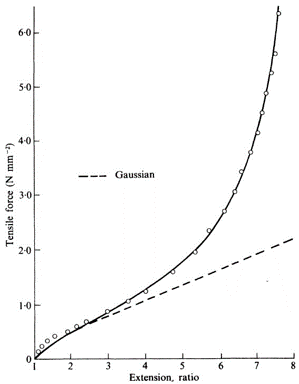
\includegraphics[height=6cm]{mooneyho-formulace}
	\caption{Aproximace experimentu Mooneyho formulací}
	\label{fig:mooneyho-formulace}
\end{figure}

\subsubsection{Rivlinova formulace (1948)}\label{subsec:rivlinova-formulace}
\begin{itemize}
	\item guma je nestlačitelná a~izotropní v~nedeformovaném stavu
	\item + logický závěr: pokud je materiál izotropní, funkce deformační energie by měla být symetrická s~ohledem na $\lambda_1$, $\lambda_2$, $\lambda_3$
	\item navrženou $W$ nesmí ovlivnit změna znaménka u~dvou $\lambda_i$ (souvisí s~rotací tělesa o~$\SI{180}{\degree}$)
\end{itemize}

Navržená $W$ by tedy měla být konvexní (polykonvexní), Rivlin navrhuje „strain ellipsoid“
\begin{itemize}
	\item Existence globálního minima energie
	\item Kladný přírůstek napětí při kladném přírůstku deformace
\end{itemize}

Pak lze zřejmě vytvořit určité vztahy, tj. invaritanty, pro $\lambda_i$.
Rivlin je navrhuje, ve formě druhých mocnin následovně:
\begin{equation}\begin{split}
	I_1 &= \lambda_1^2 + \lambda_2^2 + \lambda_3^2\\
	I_2 &= \lambda_1^2 \lambda_2^2 + \lambda_2^2 \lambda_3^2 + \lambda_3^2 \lambda_1^2\\
	I_3 &= \lambda_1^2 \lambda_2^2 \lambda_3^2
\end{split}\end{equation}

\begin{figure}[H]
	\centering
	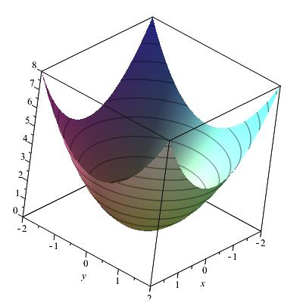
\includegraphics{rivlinova-formulace}
	\caption{Konvexní funkce}
	\label{fig:rivlinova-formulace}
\end{figure}

Nestlačitelnost umožňuje definovat předchozí dva invarianty jako:
\begin{equation}\begin{split}
	I_1 &= \lambda_1^2 + \lambda_2^2 + \lambda_3^2\\
	I_2 &= \lambda_1^2 \lambda_2^2 + \lambda_2^2 \lambda_3^2 + \lambda_3^2 \lambda_1^2 = \frac{1}{\lambda_1^2} + \frac{1}{\lambda_2^2} + \frac{1}{\lambda_3^2}
\end{split}\end{equation}

V~podobě dvou nezávislých invariantů je tak navržena i~energie napjatosti
\begin{equation}
	W = \sum\limits_{i=0, j=0}^{\infty} C_{ij} (I_1-3)^i (I_2-3)^j,
\end{equation}
přičemž $(I_1-3)$ a~$(I_2-3)$ je navrženo schválně, aby členy byly $0$ při nulových deformacích a~$C_{\infty}=0$ ze stejného důvodu.

Bohužel, bez nějaké „první“ znalosti o~křivce $\sigma-\varepsilon$ je velmi obtížné vybrat koeficienty $i$,$j$ smysluplně. Většinou se berou první členy rozvoje.

\begin{equation}\begin{split}
	i=1, j=0: \quad &W = C_{10} (I_1-3)^1 = C_{10} \left(\lambda_1^2 + \lambda_2^2 + \lambda_3^2 - 3\right) \quad \text{\ldots Neo-Hook}\\
	i=0, j=1: \quad &W = C_{01} (I_2-3)^1 = C_{01} \left(\frac{1}{\lambda_1^2} + \frac{1}{\lambda_2^2} + \frac{1}{\lambda_3^2} - 3\right) \quad \text{\ldots nemá aplikaci}
\end{split}\end{equation}
Kombinace obou dává opět \hyperref[subsec:mooneyho-formulace]{Mooneyho formulaci}. Co další kombinace?

% !TeX root = skripta-konstitutivni-vztahy.tex
% !TeX lastmodified = 2016-11-01

\subsection{Model Yeoh}\label{sec:yeoh}
\begin{itemize}
	\item YEOH (1993)
	\item vychází z Mooney-Rivlinovy formulace
	\item Yeoh dokázal, že celková energie napjatosti je více ovlivněna přírůstky $\frac{\partial W}{\partial I_1}$ než $\frac{\partial W}{\partial I_2}$ a~tedy je navržena řada v podobě:
	\begin{equation}
		W = C_{10} (I_1-3) + C_{20} (I_1-3)^2 + C_{30} (I_1-3)^3
	\end{equation}
	\item později bylo usouzeno, že se může vzít i vyšší počet členů
\end{itemize}
\begin{equation}
	W = \sum\limits_{i=1}^5 C_{i0} (I_1 - 3)^i
\end{equation}

\subsubsection{Důkaz}
Vychází se z~modelu Mooney-Rivlina (kapitola \ref{sec:mooney-rivlin})
\begin{equation}
	W = C_{10} (I_1-3) + C_{01} (I_2-3) + C_{20} (I_1-3)^2 + C_{11} (I_1-3) (I_2-3) + C_{30} (I_1-3)^3
\end{equation}
přičemž
\begin{equation*}
	\frac{\partial W}{\partial I_2} = C_{01} + C_{11} (I_2-3)
\end{equation*}
příspěvek je tedy nulový jen v případě, že $C_{01} = 0$ a~$C_{11} = 0$.

při dosazení zpět plyne původní forma konstitutivní rovnice ve tvaru:
\begin{equation}
	W = C_{10} (I_1-3) + C_{20} (I_1-3)^2 + C_{30} (I_1-3)^3
\end{equation}

\begin{figure}[H]
	\centering
	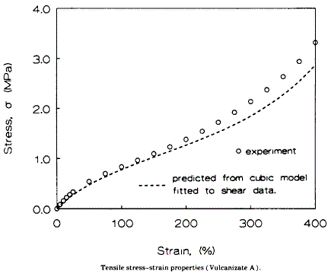
\includegraphics{yeoh-experiment-tah}
	\caption{Aproximace experimentu (tah) modelem Yeoh}
	\label{fig:yeoh-experiment-tah}
\end{figure}
\begin{figure}[H]
	\centering
	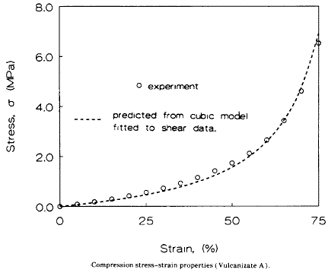
\includegraphics{yeoh-experiment-tlak}
	\caption{Aproximace experimentu (tlak) modelem Yeoh}
	\label{fig:yeoh-experiment-tlak}
\end{figure}
% !TeX root = skripta-konstitutivni-vztahy.tex
% !TeX lastmodified = 2018-10-30

\subsection{Model Arruda-Boyce}\label{sec:arruda-boyce}
Tento model\footnote{Arruda EM, Boyce  MC: A three-dimensional constitutive model for large stretch behavior of rubber elastic materials. J. Mechanics and Physics of Solids, 1993, Vol. 41/2, pp. 389-412.} na rozdíl od předchozích modelů ryze fenomenologických vychází ze struktury materiálu, tvořené vláknitými zvlněnými řetězci makromolekul elastomeru.
Při jejich protažení dochází postupně k~jejich napřimování a~tím ke zvyšování tuhosti elastomeru -- deformačnímu zpevnění.
Protože řetězce jsou v~prostoru náhodně uspořádány (izotropní materiál), vyžaduje vyčíslení jejich příspěvku k~deformační energii všesměrovou 3D integraci (přes kouli).
Pro zjednodušení byla hledána taková uspořádání vláken, která při zachování symetrie podle hlavních materiálových rovin umožní jednodušší vyčíslení.
Dříve navržená zjednodušení (třířetězcový model krychlový, čtyřřetězcový model tetraedrický) tyto požadavky nesplňovala.

\begin{figure}[H]
	\centering
	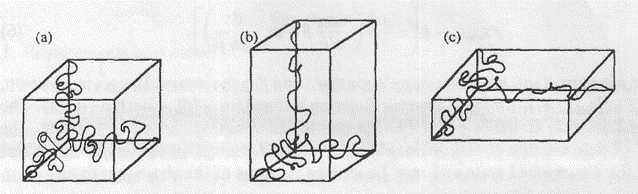
\includegraphics{triretezcovy-model-krychlovy}
	\caption{Třířetězcový model krychlový}
	\label{fig:triretezcovy-model-krychlovy}
\end{figure}

\begin{figure}[H]
	\centering
	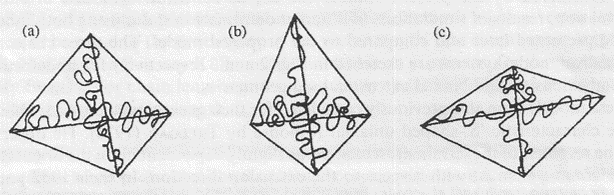
\includegraphics{ctyrretezcovy-model-tetraedricky}
	\caption{Čtyřřetězcový model tetraedrický}
	\label{fig:ctyrretezcovy-model-tetraedricky}
\end{figure}

Model Arruda-Boyce zavádí hexagonální buňku (krychli) s~rohy propojenými s~jejím středem pomocí osmi molekulárních řetězců -- proto někdy nazýván \uv{8-chain model}.

\begin{figure}[H]
	\centering
	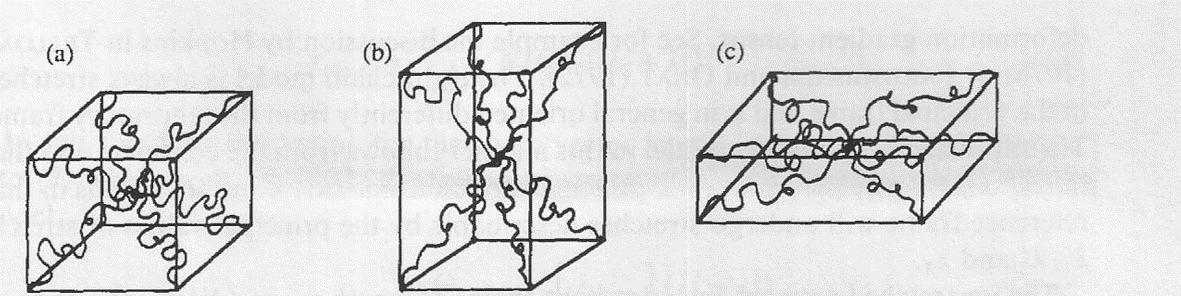
\includegraphics[width=0.75\linewidth]{osmiretezcovy-model-krychlovy}
	\caption{Osmiřetěžcový model krychlovy}
	\label{fig:osmiretezcovy-model-krychlovy}
\end{figure}

Molekulární řetězce elastomerů nejsou na rozdíl od krystalických materiálů spojeny kovalentními vazbami a~uplatňuje se u~nich jiný deformační mechanismus.
Vhodným modelem je řetězec tuhých článků vzájemně spojených rotačními vazbami, které minimalizují ohybovou tuhost řetězce.
Pak je jeho tvar výsledkem náhodných tepelných fluktuací a~o~pravděpodobnosti určitého tvaru molekulárního řetězce rozhoduje entropie -- jedná se o entropickou elasticitu.

Pro protažení řetězce definované obvyklým způsobem
\begin{equation}
	\lambda_\text{chain} = \frac{r_\text{chain}}{r_0}
\end{equation}
kde $r_0 = l \sqrt{N}$ je počáteční délka řetězce, daná statisticky délkou článku řetězce $l$ a~počtem článků $N$.
Limitní délka řetězce a~limitní protažení řetězce je pak
\begin{equation}
	r_L = l N
	\qquad
	\lambda_L = \frac{r_L}{r_0} = \sqrt{N}
\end{equation}
Model vychází z předpokladu afinní deformace (deformace řetězců-vláken je identická s~deformací okolní matrice).

Použijeme-li pro tvar řetězce Gaussovu statistiku, dostaneme pro model Neo-Hooke energii napjatosti ve tvaru:
\begin{equation}
	W = \frac{1}{2} G (\bar{I}_1 - 3)
	= \frac{1}{2} G \left(\lambda_1^2 + \lambda_2^2 + \lambda_3^2 - 3\right)
\end{equation}
kde
\begin{description}
	\item[{$G = n k_B T$}] je počáteční modul pružnosti ve smyku,
	\item[$n$] je hustota řetězce (počet řetězců v jednotkovém objemu)
	\item[$k_B$] je Boltzmannova konstanta,
	\item[$T$] je absolutní teplota.
\end{description}

Použitím Langevinovy statistiky dostaneme konfigurační entropii pro délku řetězce $r_\text{chain}$:
\begin{equation}
	S_\text{chain} = k_B \left\{c - N\left[\frac{r_\text{chain}}{N l} \beta + \ln\left(\frac{\beta}{\sinh(\beta)}\right) \right]\right\}
\end{equation}
kde $c$ je konstanta a~$\beta$ je inverzní Langevinova funkce definovaná vztahem
\begin{equation}
	\beta = \Im\left(\frac{r_\text{chain}}{N l}\right)
\end{equation}
pro
\begin{equation}
	\Im(\beta) = \coth(\beta) - \frac{1}{\beta}
\end{equation}

Použití Langevinovy statistiky umožňuje správně započítat limitní protažení strukturních řetězců $\lambda_L$. Deformační práce při izotermickém ději je pak úměrná změně entropie při protažení řetězců a~dá se vyjádřit následovně
\begin{equation}\label{eq:deformacni-prace-izotermickeho-deje}
	W = n k_B T N \left[\frac{r_\text{chain}}{N l} \beta + \ln\left(\frac{\beta}{\sinh(\beta)}\right) \right]
	= G \lambda_L \left\{ \lambda_\text{chain} \beta - \lambda_L \ln\left[ \frac{\sinh(\beta)}{\beta} \right] \right\}
\end{equation}

Složky napětí dostaneme standardním způsobem derivací podle složek deformačního tenzoru. Protože materiál je nestlačitelný, figuruje ve vztahu hydrostatický tlak jako další proměnná (Lagrangeův multiplikátor), která se musí určit z~okrajových podmínek.

Deformace různě orientovaných řetězců je při každém deformačním stavu různá, takže pro určení celkové deformační práce je nutné pro každý takový stav provádět integraci přes distribuci různě orientovaných řetězců.
Při deformaci dochází k~rotaci jednotlivých řetězců, takže pro určení jejich protažení (stretch tensor) je třeba provést polární dekompozici tenzoru deformačního gradientu a~poté určit hlavní souřadnice tenzoru protažení.
Derivací této práce podle hlavních protažení (hlavní složky tenzoru protažení) dostaneme 1.~Piola-Kirchhoffovo napětí a~následně skutečné napětí $\sigma_i$:
\begin{equation}
	\sigma_i = \lambda_i \frac{\diff W}{\diff \lambda_i} + p
\end{equation}
kde $p$ je Lagrangeův multiplikátor s~fyzikálním významem tlaku, který se určí z~okrajových podmínek. Ten lze eliminovat vyjádřením rozdílu hlavních napětí
\begin{equation}
	\sigma_1 - \sigma_2 = \lambda_1 \frac{\diff W}{\diff \lambda_1} - \lambda_2 \frac{\diff W}{\diff \lambda_2}
\end{equation}

Výhodou modelu je kromě (kubické) symetrie podle všech hlavních rovin, že všechny řetězce jsou při jakémkoli deformačním stavu protahovány (dáno podmínkou nestlačitelnosti materiálu).

V~nedeformovaném stavu je délka kteréhokoli z~řetězců v krychli o~hraně $a_0$ dána vztahem:
\begin{equation}
	2 r_0 = \sqrt{3 a_0^2} = \sqrt{3} a_0
	\quad\Rightarrow\quad
	r_0 = \frac{\sqrt{3}}{2} a_0
\end{equation}
Vektorově je ho možné napsat v~hlavním souřadnicovém systému tenzoru protažení (konkrétně pro řetězec směřující do 1.~kvadrantu):
\begin{equation}
	\vec{r}_0 = \frac{a_0}{2} \vec{i} + \frac{a_0}{2} \vec{i} + \frac{a_0}{2} \vec{k}
\end{equation}

V~deformovaném stavu bude vektorový zápis:
\begin{equation}
	\vec{r}_\text{chain} = \lambda_1 \frac{a_0}{2} \vec{i} + \lambda_2 \frac{a_0}{2} \vec{i} + \lambda_3 \frac{a_0}{2} \vec{k}
\end{equation}
a~velikost vektoru řetězce v~deformovaném stavu bude
\begin{equation}
	r_\text{chain} = \frac{a_0}{2} \sqrt{\lambda_1^2 + \lambda_2^2 + \lambda_3^2}
\end{equation}
Pak protažení tohoto řetězce je
\begin{equation}\label{eq:protazeni-retezce}
	\lambda_\text{chain}
	= \frac{r_\text{chain}}{r_0}
	= \frac{\sqrt{\lambda_1^2 + \lambda_2^2 + \lambda_3^2}}{\sqrt{3}}
	= \sqrt{\frac{I_1}{3}}
\end{equation}
Dosazením (\ref{eq:protazeni-retezce}) do (\ref{eq:deformacni-prace-izotermickeho-deje}) dostaneme energii $W$ jako funkci $I_1$.

Aplikujeme-li nyní pro popis náhodné prostorové distribuce řetězců polynomický rozvoj inverzní Langevinovy funkce a~použijeme jeho prvních pět členů, dostaneme deformační energii:
\begin{multline}
	W
	= n k_B T \left[ \frac{1}{2} (\bar{I}_1-3) + \frac{1}{20 N} (\bar{I}_1^2-9) + \frac{11}{1050 N^2} (\bar{I}_1^3-27) \right.\\
	\left. + \frac{19}{7000 N^3} (\bar{I}_1^4-81) + \frac{519}{673750 N^4} (\bar{I}_1^5-243) \right]
\end{multline}

Dosazením dříve odvozeného vztahu $\alpha_L = \sqrt{N} \Rightarrow N = \lambda_L^2$ a~přidáním členu popisujícího energii objemové části deformace dostaneme výsledný vztah:
\begin{multline}
	W
	= G \left[ \frac{1}{2} (\bar{I}_1-3) + \frac{1}{20 \lambda_L^2} (\bar{I}_1^2-9) + \frac{11}{1050 \lambda_L^4} (\bar{I}_1^3-27) \right.\\
	\left. + \frac{19}{7000 \lambda_L^6} (\bar{I}_1^4-81) + \frac{519}{673750 \lambda_L^8} (\bar{I}_1^5-243) \right]
	+ \frac{1}{d} \left(\frac{J^2 - 1}{2} - \ln(J)\right)
\end{multline}
kde $d=\frac{2}{K}$.

Pro $\lambda_L \rightarrow \infty$ se model redukuje na model \hyperref[sec:neo-hooke]{Neo-Hooke}.

\subsubsection{Výhody modelu Arruda-Boyce}
\begin{itemize}
	\item Model je téměř izotropní (nepatrná závislost na orientaci reprezentativní krychle resp. řetězců vůči směru zatížení) a~má vysokou míru symetrie vůči hlavním rovinám protažení.
	\item V~každém zatěžovacím stavu se všechny řetězce podílejí na přenosu zatížení. Jejich protažení se vzájemně liší a~díky jejich natáčení limitní protažení struktury přesahuje limitní protažení řetězce $\lambda_L$, které je však rozhodující pro zpevňování v~kterémkoli směru a~deformačním modu.
	\item Model má pouze 2 materiálové parametry pro deviátorovou část a~je schopen popsat zatěžovací křivku s~inflexí (zpevňující).
	\item Na rozdíl od fenomenologických modelů mají oba parametry jasně definovaný fyzikální význam.
	\item Díky strukturní povaze modelu má výbornou predikční schopnost; i~když použijeme pro určení jeho parametrů jen určitý typ napjatosti (např. jednoosou tahovou), dává rozumné výsledky i~pro jiné typy napjatosti.
\end{itemize}

\begin{figure}[H]
	\centering
	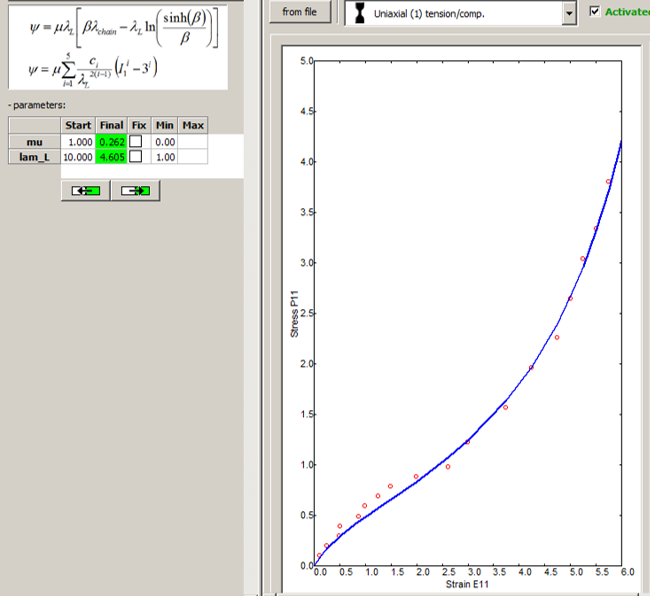
\includegraphics[width=0.5\linewidth]{aproximace-arruda-boyce}
	\caption{Proložení reálné experimentální křivky modelem Arruda-Boyce}
	\label{fig:aproximace-arruda-boyce}
\end{figure}

% !TeX root = skripta-konstitutivni-vztahy.tex
% !TeX lastmodified = 2018-11-07

\subsection{Co je to predikční schopnost?}
Nejsou-li k~dispozici všechny potřebné mechanické zkoušky při různých typech napjatosti, je model nedostatečně experimentálně podložen.
Nejčastěji jsou konstanty modelu určeny jen z~jednoosé tahové zkoušky a~model musí predikovat (předpovědět) chování materiálu při jiném (víceosém) typu napjatosti. Přesnost, s~jakou to model dokáže, se nazývá jeho predikční schopností.

Odhad polohy deformačně-napěťových křivek ve dvouosé napjatosti vůči křivce určené z~jednoosé tahové zkoušky je možno udělat pro malé deformace z~Hookova zákona
\begin{equation}
	\sigma_1 = 2 G \varepsilon_1 + \lambda e = 2 G \varepsilon_1 + \lambda \left( \varepsilon_1 + \varepsilon_2 + \varepsilon_3 \right)
\end{equation}

Při tahovém zatížení ve směru 1 je tedy tuhost v~tomto směru při rovinné deformaci ($\varepsilon_2 = 0$) vždy větší než při jednoosé napjatosti (zde je $\varepsilon_2$ záporné a~tuhost odpovídá modulu pružnosti $E = \frac{\sigma_1}{\varepsilon_1}$). 
Při dvouosé napjatosti ($\varepsilon_2$ kladné) pak je tuhost ještě vyšší.
Pouze pro úplnou nestlačitelnost materiálu ($e = 0$) jsou odezvy při všech uvedených zkouškách (v~oblasti malých přetvoření) stejné.

Odezva izotropního materiálu při dvouosé napjatosti tedy není nikdy poddajnější než při jednoosé napjatosti.
Na druhé straně také nebývá mnohonásobně tužší.

\subsubsection{Predikční schopnost modelu Arruda-Boyce}
\begin{figure}[H]
	\centering
	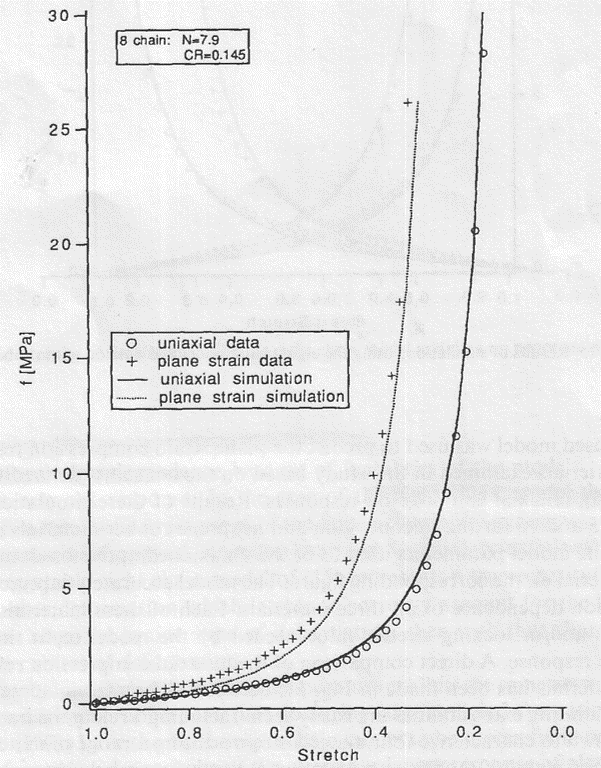
\includegraphics[height=5cm]{konstanty-tlak-arruda-boyce}
	\caption{Konstanty modelu určeny pouze z jednoosé tlakové zkoušky}
	\label{fig:konstanty-tlak-arruda-boyce}
\end{figure}
\begin{figure}[H]
	\centering
	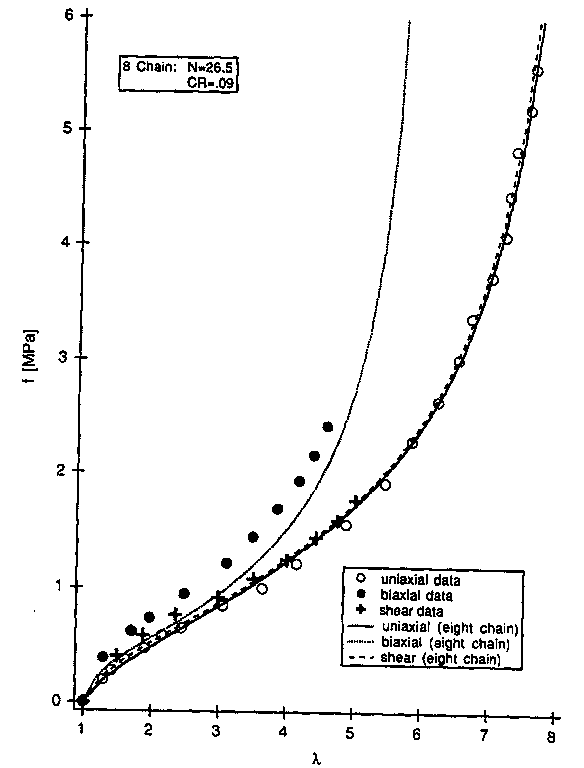
\includegraphics[height=5cm]{konstanty-tah-arruda-boyce}
	\caption{Konstanty modelu určeny pouze z jednoosé tahové zkoušky}
	\label{fig:konstanty-tah-arruda-boyce}
\end{figure}
% !TeX root = skripta-konstitutivni-vztahy-materialu.tex
% !TeX lastmodified = 2019-11-06

\subsection{Model Ogden pro pěnové pryže}\label{sec:ogden-foam}
Tento model zavádí energii napjatosti ve tvaru
\begin{equation}
	W
	= \sum\limits_{i=1}^N \frac{\mu_i}{\alpha_i} \left( \bar{\lambda}_1^{\alpha_i} + \bar{\lambda}_2^{\alpha_i} + \bar{\lambda}_3^{\alpha_i} - 3 \right)
	+ \sum\limits_{i=1}^N \frac{\mu_i}{\beta_i} \left(1 - J^{\beta_i}\right),
\end{equation}
nebo pro velmi stlačitelné elastomery svazuje objemovou a~deviátorovou část energie napjatosti vztahem (použit v~ANSYSu)
\begin{equation}
	W
	= \sum\limits_{i=1}^N \frac{\mu_i}{\alpha_i} \left[ J^{\frac{\alpha_i}{3}} \left( \bar{\lambda}_1^{\alpha_i} + \bar{\lambda}_2^{\alpha_i} + \bar{\lambda}_3^{\alpha_i} \right) - 3 \right]
	+ \sum\limits_{i=1}^N \frac{\mu_i}{\alpha_i \beta_i} \left(J^{-\alpha_i \beta_i} - 1\right),
\end{equation}
kde
\begin{description}
	\item[$\mu_i, \alpha_i, \beta_i$] jsou materiálové parametry,
	\item[$\bar{\lambda}_i (i=1,2,3)$] = modifikovaná hlavní poměrná protažení,
	\item[$J$] je třetí invariant tenzoru deformačního gradientu.
\end{description}

Pro $\beta_i = 0$ dostaneme nestlačitelný model \hyperref[sec:model-ogden]{Ogden}.

Model je použitelný jen v~tlaku ($J < 1$) (u~pěny se nepředpokládá).

\subsection{Model Blatz-Ko pro pěnové pryže}\label{sec:blatz-ko}
Tento model navržený pro pěnové pryže zavádí měrnou energii napjatosti ve tvaru
\begin{equation}
	W = \frac{G}{2} \left( \frac{I_2}{I_3} + 2 \sqrt{I_3} - 5 \right),
\end{equation}
kde
\begin{description}
	\item[$G$] je modul pružnosti ve smyku,
	\item[$I_2, I_3$] jsou invarianty pravého Cauchy-Greenova tenzoru deformace.
\end{description}

\section{Modely neelastického chování}
% !TeX root = skripta-konstitutivni-vztahy.tex
% !TeX lastmodified = 2018-11-27

\subsection{Průběhy tlakové zkoušky pro různé druhy gumy}
\begin{figure}[H]
	\centering
	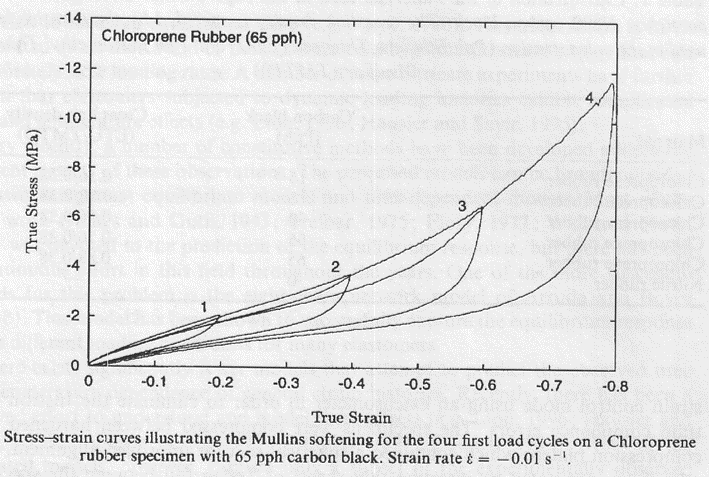
\includegraphics[width=0.7\linewidth]{mullinsovy-efekt-vyrazny}
	\caption{Guma s~velkým obsahem plniva vykazuje významný Mullinsův efekt a~významnou hysterezi (viskoelasticitu).}
	\label{fig:mullinsovy-efekt-vyrazny}
\end{figure}

Mullinsův effekt je změkčení materiálu vlivem předchozího zatížení, při němž dojde k~poškození vzájemných vazeb (zesíťování) mezi vlákny v~materiálu. To se projeví při následujících zatěžovacích cyklech nižší tuhostí materiálu, dokud se nedosáhne maximální hodnoty deformace (deformační energie) z~předchozího zatěžování. Nad touto hodnotou se materiál vrací na tzv. \uv{panenskou} křivku prvního cyklu.

\begin{figure}[H]
	\centering
	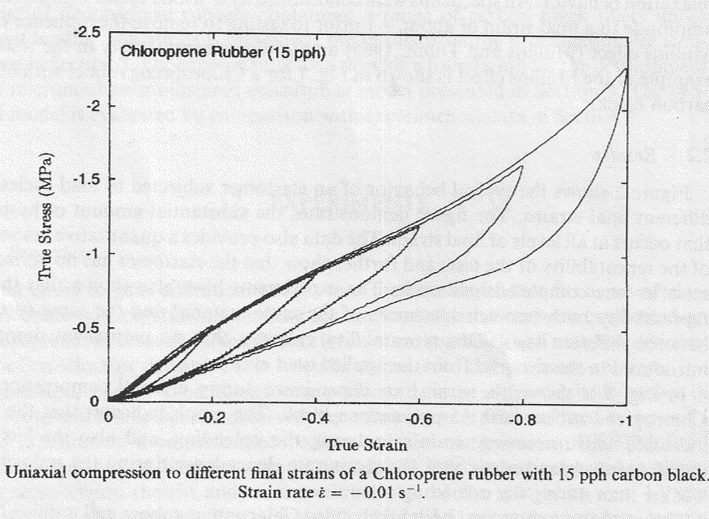
\includegraphics[width=0.7\linewidth]{mullinsovy-efekt-nevyrazny}
	\caption{Guma s~malým množstvím plniva, nepatrným Mullinsovým efektem, ale významnou hysterezí.}
	\label{fig:mullinsovy-efekt-nevyrazny}
\end{figure}

\begin{figure}[H]
	\centering
	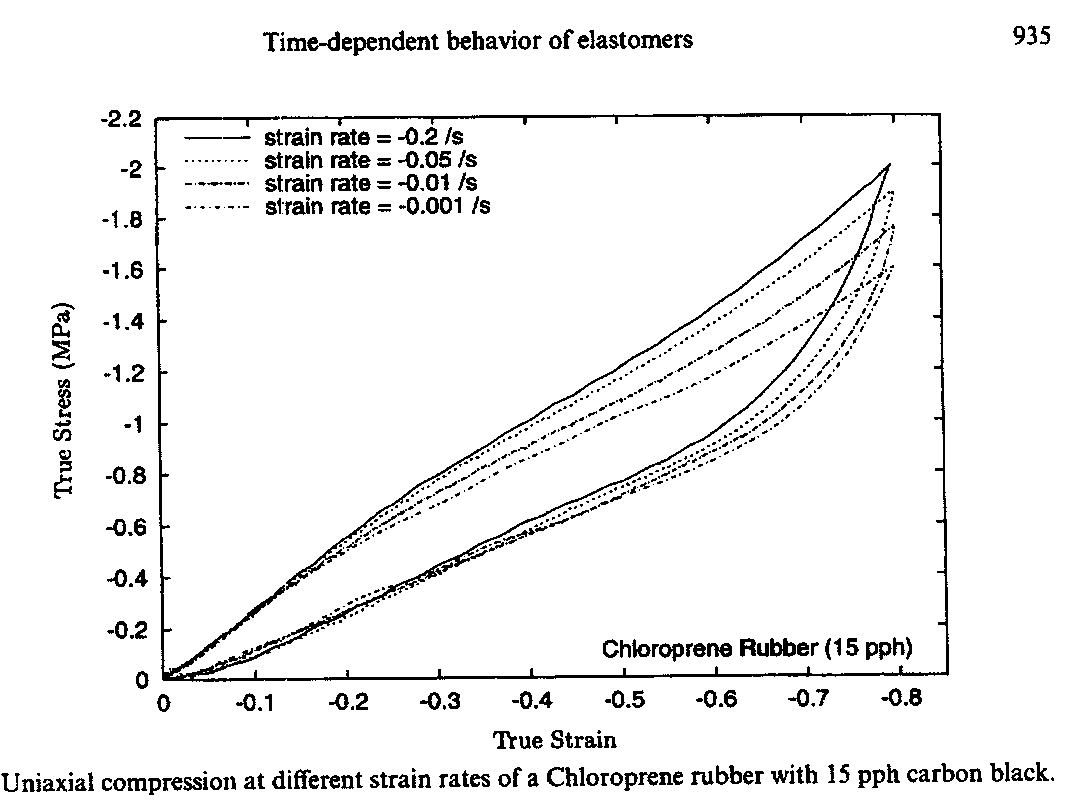
\includegraphics[width=0.7\linewidth]{visko-hyperelasticita}
	\caption{Tlakové zkoušky pro chloroprenovou gumu při různých rychlostech zatěžování -- visko-hyperelasticita}
	\label{fig:visko-hyperelasticita}
\end{figure}

% !TeX root = skripta-konstitutivni-vztahy-materialu.tex
% !TeX lastmodified = 2019-11-20

\subsection{Model Ogden-Roxburgh}\label{sec:ogden-roxburgh}
Tento pseudoelastický model\footnote{Ogden RW, Roxburgh DG (1999): A pseudo-elastic model for the Mullins effect in filled rubber. Proc. Royal Society London A, Vol. 455, pp. 2861-2877.} byl navržen v~roce 1999 pro popis Mullinsova efektu, který je významný zvláště u~plněných elastomerů.
Model sestává z~funkce měrné energie napjatosti $\psi_0$ pro popis panenské materiálové křivky, která se modifikuje při odlehčovacím a~dalších zatěžovacích cyklech korekčním faktorem (damage parameter) $\eta$, snižujícím úroveň napětí v~závislosti na předcházející maximální hodnotě zatížení $\psi_0^\text{max}$:
\begin{align}
	\psi(\bm{F}, \eta) &= \eta \psi_0(\bm{F}) + \varPhi(\eta),\\
	\eta &= 1 - \frac{1}{r} \mathrm{erf}\left( \frac{\psi_0^\text{max} - \psi_0}{m + \beta \psi_0^\text{max}} \right),
\end{align}
kde
\begin{description}
	\item[$\mathrm{erf}()$] označuje \hyperref[sec:chybova-funkce]{chybovou funkci} (error function),
	\item[$\bm{F}$] je tenzor deformačního gradientu,
	\item[$\varPhi(\eta)$] je korekční funkce zajišťující, aby se faktorem $\eta$ redukovalo napětí (získané parciální derivací podle složky přetvoření) a~nikoli hustota deformační energie,
	\item[{$r\:[-] \geq 1$}] je materiálový parametr určující míru poškození (snížení napětí) vůči panenskému stavu  materiálu,
	\item[{$m\:[Pa]$}] je materiálový parametr určující závislost poškození (snížení napětí) na rozsahu předchozí deformace (strmost návratu k~panenské křivce, příkrá pro nízká $m$, pozvolná pro vysoká $m$),
	\item[{$\beta\:[-]$}] je materiálový parametr měnící strmost návratu k~panenské křivce v~závislosti na velikosti předchozího zatížení.
\end{description}

\subsubsection{Vlastnosti modelu}
Tento pseudoelastický model (v~ANSYSu označovaný jako CDF -- continuum damage function) je založen na korekčním faktoru (damage parameter) $\eta$, který snižuje napětí při daném přetvoření v~závislosti na maximální deformační energii (resp. max. přetvoření) dosažené v předchozí historii zatěžování.

Tato korekční funkce je specifická pro každý element modelu (přesněji pro každý integrační bod), podle jeho předchozí maximální deformační energie, tedy nezávisle na specifickém deformačně-napěťovém stavu.
Teprve je-li toto maximum překročeno, pokračuje zatěžovací proces po panenské křivce a~odlehčovací křivka se následně změní.

Model z~principu není schopen postihnout:
\begin{itemize}
	\item rozdíl mezi odlehčovací a~následnou zatěžovací křivkou (hysterezi v~opakovaných zátěžných cyklech,
	\item trvalou plastickou deformaci,
	\item spojitý a~hladký přechod z~korigované na panenskou křivku; na rozdíl od reality nastává při přechodu její zlom (nespojitost derivace).
\end{itemize}

\begin{figure}[H]
	\centering
	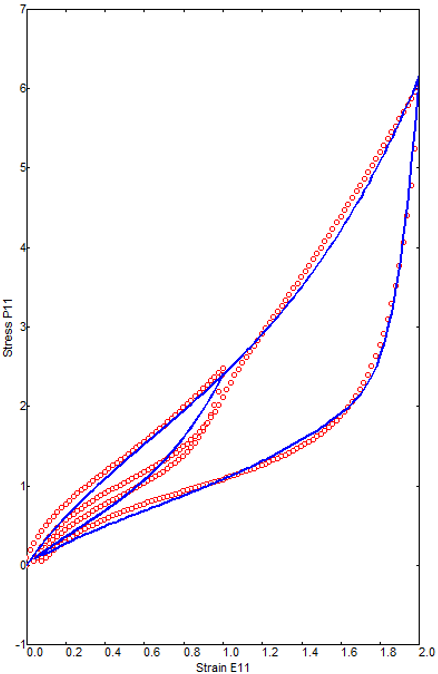
\includegraphics[height=6cm]{aproximace-ogden-roxburgh}
	\caption{Aproximace experimentu modelem Ogden-Roxburgh}
	\label{fig:aproximace-ogden-roxburgh}
\end{figure}

% !TeX root = skripta-konstitutivni-vztahy-materialu.tex
% !TeX lastmodified = 2019-11-27

\subsection{Model Bergstr\H{o}m-Boyce}\label{sec:bergstrom-boyce}
Tento model\footnote{Bergström JS, Boyce MC (1998):  Constitutive Modeling of the Large Strain Time-dependent Behavior of Elastomers, Journal of the Mechanics and Physics of Solids 45 (5), pp. 931-954.}\footnote{Bergström, J. S., Boyce, M. C. (2001): Constitutive Modeling of the Time-Dependent and Cyclic Loading of Elastomers and Application to Soft Biological Tissues, Mechanics of Materials 33, pp. 523-530.} byl navržen v~roce 1998 pro popis časově závislého chování elastomerů ve velkých deformacích.
Vychází z~hyperelastického modelu Arruda-Boyce a~rozšiřuje jej o~popis závislosti mechanické odezvy na rychlosti deformace (viskohyperelasticitu);
tím umožňuje popsat hysterezi deformačně-napěťových křivek, stejně jako tečení a~relaxaci napětí.

Podobně jako model Arruda-Boyce vychází z~modelu prostorové sítě makromolekulárních řetězců, jejichž deformace je řízena entropickou elasticitou.
K~původní osmiřetězcové síti modelu Arruda-Boyce, popisující hyperelastickou odezvu, tedy termodynamicky rovnovážný stav, přidává druhou síť reprezentující odchylky od rovnovážného stavu.
Odpovídá to reologickému modelu Kelvin (standard linear solid), kde řetězec~A reprezentuje rovnovážnou část deformační práce a~řetězec~B nerovnovážnou část.
\begin{figure}[H]
	\centering
	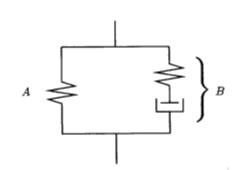
\includegraphics[height=3cm]{kelvinuv-model-ab}
	\caption{Kelvinův reologický model}
	\label{fig:kelvinuv-model-ab}
\end{figure}

\subsubsection{Dekompozice deformačního tenzoru}
Paralelní části reologického modelu mají stejnou deformaci, tedy platí
\begin{equation}
	\bm{F} = \bm{F}_A = \bm{F}_B
\end{equation}

Pro řetězec~B lze deformaci rozložit na část elastickou a~neelastickou (viskózní)
\begin{equation}
	\bm{F}^B = \bm{F}^B_\text{el} \bm{F}^B_\text{vis}
\end{equation}

Na každý z~deformačních tenzorů je možné aplikovat jeho polární dekompozici (viz obr.)
\begin{figure}[H]
	\centering
	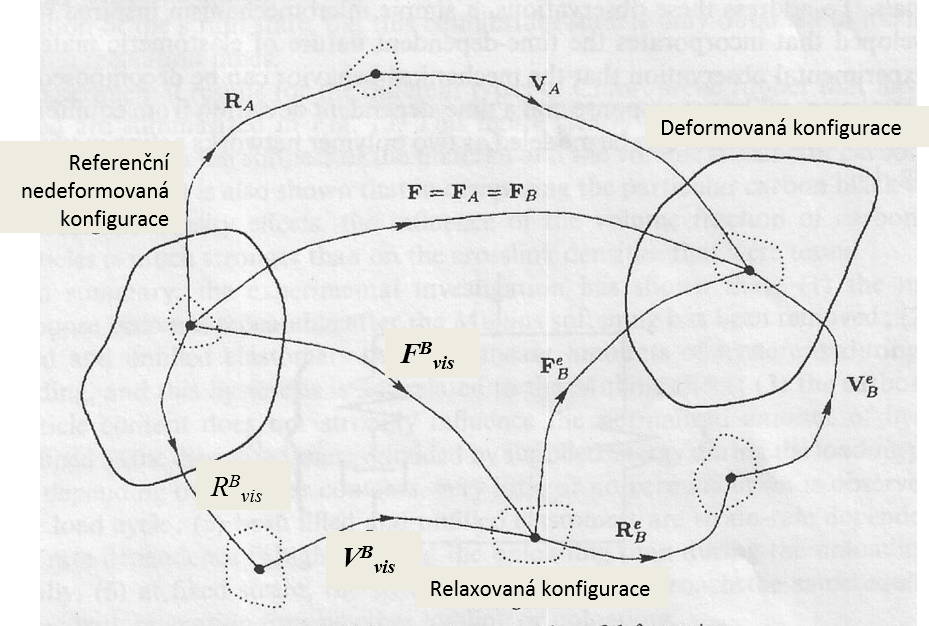
\includegraphics[width=0.7\linewidth]{polarni-dekompozice}
	\caption{Polární dekompozice}
	\label{fig:polarni-dekompozice}
\end{figure}

\subsubsection{Princip relaxace modelu Bergstr\H{o}m-Boyce}
Relaxaci napětí lze nejsnadněji vysvětlit existencí volného řetězce v~síti makromolekul, jehož deformace se \enquote{plazivým} pohybem pomalu vrací do více zvlněného (a~tedy přirozenějšího) stavu.
\begin{figure}[H]
	\centering
	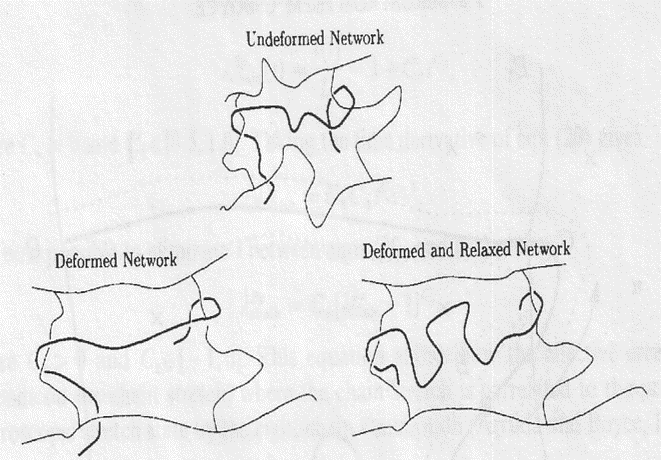
\includegraphics[width=0.7\linewidth]{volny-retezec}
	\caption{Volný řetězec v~síti}
	\label{fig:volny-retezec}
\end{figure}

Přestože se volné řetězce v~makromolekulární síti  elastomerů nevyskytují, mohou tam existovat téměř volné (náhodně ohnuté) konce řetězců (obr. vpravo), které se chovají podobně.
Po deformaci se napnou a~postupně se vracejí do více zvlněného stavu s~vyšší entropií.
\begin{figure}[H]
	\centering
	\includegraphics[width=0.7\linewidth]{temer-volne-konce-retezcu}
	\caption{Téměř volné konce řetězců}
	\label{fig:temer-volne-konce-retezcu}
\end{figure}

\subsubsection{Rovnice modelu Bergstrőm-Boyce}
Pro část~A podle reologického schématu se používá popis Arruda-Boyce, viz rov. (\ref{eq:deformacni-prace-izotermickeho-deje})
\begin{equation}
	W^A = G^A \lambda_L^A \left\{ \lambda_\text{chain} \beta^A - \lambda_L^A \ln\left[ \frac{\sinh\left(\beta^A\right)}{\beta^A} \right] \right\}
\end{equation}

Pro popis části~B se po dekompozici deformačního gradientu na elastickou a~viskózní část použije pro elastickou část~B analogická rovnice jako pro~A
\begin{equation}
	W_\text{el}^B = G^B \lambda_L^B \left\{ \lambda_\text{chain}^\text{el} \beta^B - \lambda_L^B \ln\left[ \frac{\sinh\left(\beta^B\right)}{\beta^B} \right] \right\},
\end{equation}
zatímco viskózní část je popsána následujícím vztahem mezi napětím a~rychlostí deformace
\begin{equation}
	\dot{\gamma} = \gamma_0 \left( \varepsilon_\text{chain}^\text{vis} \right)^C \left( \frac{\tau}{\tau_\text{base}} \right)^m,
\end{equation}
který lze upravit do tvaru používaného v~ANSYSu:
\begin{equation}
	\dot{\gamma} = \frac{\gamma_0}{\tau_\text{base}^m} \left( \lambda_\text{chain}^\text{vis} - 1 + \delta \right)^C \tau^m.
\end{equation}
ANSYS zde využívá ještě rovnici
\begin{equation}
	\lambda_L = \sqrt{N}.
\end{equation}

\subsubsection{Konstanty modelu Bergstrőm-Boyce v~ANSYSu}
Dohromady je ve všech třech částech modelu (reologického schématu) těchto 7 materiálových parametrů (značení podle ANSYSu):
\begin{figure}[H]\label{tab:konstanty-bergstrom-boyce}
	\centering
	\begin{tabular}{ll}\toprule
		Počáteční smykový modul části A & $G_A$ ('C1')\\
		Počet článků řetězce části A & $N_A$ ('C2')\\
		Počáteční smykový modul části B & $G_B$ ('C3')\\
		Počet článků řetězce části B & $N_B$ ('C4')\\
		Creepový parametr & $\tfrac{\gamma_0}{\tau_\text{base}^m}$ ('C5')\\
		Exponent creepové deformace & $C$ ('C6')\\
		Exponent efektivního napětí & $m$ ('C7')\\
	\bottomrule\end{tabular}
\end{figure}

$\delta$ ve vztahu pro viskózní část je matematická konstanta o~malé hodnotě (typicky $\delta \leq \num{0.01}$), která odstraňuje singularitu napětí pro nulové deformace.

\begin{figure}[H]
	\centering
	\includegraphics[width=0.9\linewidth]{aproximace-bergstrom-boyce}
	\caption{Aproximace jednoosé tlakové zkoušky s~relaxací během zatěžování i~odlehčování při různých rychlostech deformace}
	\label{fig:aproximace-bergstrom-boyce}
\end{figure}

% !TeX root = skripta-konstitutivni-vztahy.tex
% !TeX lastmodified = 2018-11-27

\subsection{Chybová funkce (error function)}\label{sec:chybova-funkce}
\begin{itemize}
	\item vychází z~distribuční funkce (CDF),
	\item používá se ve statistice pro predikci chování nějakého vzorku vzhledem ke střední hodnotě souboru.
\end{itemize}

\subsubsection{Vztah CDF a~hustoty pravděpodobnosti}
Funkce hustoty pravděpodobnosti $f_x$ s~mediánem $\mu$ a~směrodatnou odchylkou $\sigma$ je v~relaci s CDF vztahem
\begin{equation}
	F_x(x) = \int\limits_{-\infty}^x f_x(t) \diff t
\end{equation}

\begin{figure}[H]
	\centering
	\includegraphics[width=0.7\linewidth]{hustota-pravdepodobnosti}
	\caption{funkce hustoty pravděpodobnosti}
	\label{fig:hustota-pravdepodobnosti}
\end{figure}

\begin{figure}[H]
	\centering
	\includegraphics[width=0.7\linewidth]{distribucni-funkce}
	\caption{cumulative distribution function (CDF)}
	\label{fig:distribucni-funkce}
\end{figure}

Chybová funkce vyhodnocená (za podmínky normálního Gaussova rozdělení chyb se směrodatnou odchylkou $\sigma$) pro $\tfrac{x}{\sigma \sqrt{2}}$ udává pro absolutní hodnoty $x$ pravděpodobnost, že měření leží ve vzdálenosti menší než $x$ od střední hodnoty.
\begin{figure}[H]
	\centering
	\includegraphics[width=0.7\linewidth]{chybova-funkce}
	\caption{Grafické znázornění chybové funkce}
	\label{fig:chybova-funkce}
\end{figure}

\subsubsection{Matematické vyjádření chybové funkce}
Byla zavedena v~matematice (nazývaná také Gauss error function) je speciální neelementární funkce sigmoidního tvaru, vyskytující se v~pravděpodobnosti, statistice nebo parciálních diferenciálních rovnicích popisujících difuzi.
Je definována takto:
\begin{equation}
	\mathrm{erf}(x) = \frac{2}{\sqrt{\pi}} \int\limits_0^x \exp\left(-t^2\right) \diff t.
\end{equation}

Byla zavedena v~teorii měření (využívající statistiku a~pravděpodobnost) a~název se používá i~při jejím přenosu do jiných oblastí matematiky, které nemají žádný vztah k~charakteristikám chyb měření.

Chybová funkce se vztahuje k~rozdělení měrné energie napjatosti $\varPhi$ (prostřednictvím integrálu normálního rozdělení) rovnicí
\begin{equation}
	\varPhi(x) = \frac{1}{2} + \frac{1}{2} \mathrm{erf}\left(\frac{x}{\sqrt{2}}\right),
\end{equation}
čímž měníme rozsah hodnot z~intervalu $\langle -1;1 \rangle$ na interval $\langle 0;1 \rangle$.

% !TeX root = skripta-konstitutivni-vztahy.tex
% !TeX lastmodified = 2018-11-20

\subsection{Anizotropní hyperelastické modely}\label{sec:anizotropni-hyperelasticke-modely}
Používají se pro popis chování vláknových kompozitů s~elastomerovou matricí (nejčastěji guma) vyztuženou vlákny.
V~základní verzi předpokládají rovnoměrné rozložení maximálně dvou osnov rovnoběžných vláken s~nulovou ohybovou tuhostí.
Předpokládají tedy nekonečně malý průměr vláken, prakticky se dají použít pro vlákna textilní nebo kovová ve formě splétaného lanka.
Pro vlákna s~významnou ohybovou tuhostí (například ocelové dráty v běhounové vrstvě některých pneumatik) jsou potřebné složitější konstitutivní modely (např. založené na Cosseratově teorii elasticity).

Pro matematický popis příspěvku vláken k~měrné energii napjatosti kompozitu používají další invarianty deformačního tenzoru. Obvykle se používají invarianty (nazývané také „pseudoinvarianty“) pravého Cauchy-Greenova tenzoru deformace $\bm{C}$, označované symboly $I_4$--$I_9$ v~jeho modifikované podobě, tedy popisující pouze deviátorovou složku deformace.

Podobně jako u~izotropních elastomerů se měrná energie skládá z~části objemové $W_\text{vol}$ a~části deviátorové (izovolumické) $W_\text{dev}$, která se dá dále rozložit na izotropní příspěvek matrice $W_\text{iso}$ a~anizotropní příspěvek vláken $W_\text{aniso}$.
\begin{equation}
	W = W_\text{vol}(J) + W_\text{dev}(\bm{C},\bm{A},\bm{B}) = W_\text{vol}(J) + W_\text{iso}(\bm{C}) + W_\text{aniso}(\bm{C},\bm{A},\bm{B}).
\end{equation}

Pro izotropní část energie napjatosti $W_\text{iso}$ lze použít kterýkoli adekvátní model (\hyperref[sec:neo-hooke]{neo-Hooke}, \hyperref[sec:mooney-rivlin]{Mooney-Rivlin}, \ldots), pro anizotropní část $W_\text{aniso}$ se zavádějí nejčastěji modely polynomické, příp. exponenciální (pro měkké biologické tkáně). $\bm{A}$ a~$\bm{B}$ zde představují takzvané „strukturní tenzory“ definující směry dvou osnov vláken.

\subsubsection{Polynomický anizotropní hyperelastický model}\label{sec:polynomicky-anizotropni-hyperelasticky-model}
Tento model je naprogramován v~ANSYSu v následujícím tvaru:
\begin{equation}
	W = W_\text{dev} + \frac{1}{d} \left(J-1\right)^2
\end{equation}

Pro objemovou část energie napjatosti je zde použit model formulovaný pro izotropní matrici, zatímco deviátorová část měrné energie napjatosti $W_\text{dev}$ je popsána takto:
\begin{equation}\begin{split}
	W_\text{dev}(\bar{\bm{C}},\bm{A},\bm{B})
	= &\sum\limits_{i=1}^3 \left(\bar{I}_1 - 3\right)^i
	+ \sum\limits_{j=1}^3 \left(\bar{I}_2 - 3\right)^j
	+ \sum\limits_{k=1}^6 \left(\bar{I}_4 - 3\right)^k\\
	+ &\sum\limits_{l=1}^6 \left(\bar{I}_5 - 3\right)^l
	+ \sum\limits_{m=1}^6 \left(\bar{I}_6 - 3\right)^m
	+ \sum\limits_{n=1}^6 \left(\bar{I}_7 - 3\right)^n
	+ \sum\limits_{o=1}^6 \left(\bar{I}_8 - 3\right)^o,
\end{split}\end{equation}
kde
\begin{description}
	\item[$a_i, b_j$] jsou materiálové parametry izotropní části (matrice) $W_\text{iso}$,
	\item[$c_k, d_l, e_m, f_n, g_o$] jsou materiálové parametry anizotropní části (vláken) $W_\text{aniso}$,
	\item[$\bar{I}_1, \bar{I}_2$] jsou redukované invarianty pravého Cauchy-Greenova tenzoru deformace $\bm{C}$,
	\item[$\bar{I}_4, \bar{I}_5, \bar{I}_6, \bar{I}_7, \bar{I}_8, \bar{I}_9$] jsou pseudoinvarianty deformačního tenzoru $\bm{C}$ a~strukturních tenzorů $\bm{A}$ a~$\bm{B}$, zatímco $I_9$ je jen konstanta zajišťující nulovou energii v~nedeformovaném stavu.
\end{description}

Model kromě prvních dvou členů využívá pouze sudé mocniny invariantů, takže zahrnuje ve své deviátorové části celkem 21 materiálových parametrů.

\subsubsection{Zjednodušení polynomického modelu}
Pro praktické použití je třeba zvolit jednodušší verzi modelu, aby se daly z~experimentu určit jeho parametry.
Nejjednodušší formulaci dostaneme, pokud pro izotropní část (matrici) použijeme model \hyperref[sec:neo-hooke]{neo-Hooke} (obvykle akceptovatelný, protože  vlákna neumožňují extrémně velké deformace) a~pro obě osnovy vláken zvolíme jednoparametrickou formulaci:
\begin{equation}
	W_\text{dev}(\bar{\bm{C}},\bm{A},\bm{B})
	= a_1 \left(\bar{I}_1 - 3\right)
	+ c_1 \left(\bar{I}_4 - 3\right)^2
	+ e_1 \left(\bar{I}_6 - 3\right)^2
\end{equation}

Ještě jednodušší forma modelu existuje pro jednosměrový kompozit, tedy s~jedinou osnovou vláken; pak poslední člen uvedené rovnice vypadne. Jsou-li naopak obě osnovy vláken identické co do tuhosti vláken a~jejich obsahu v~materiálu (včetně rozložení po tloušťce, které je ovšem předpokládáno ideálně rovnoměrné), pak platí $e_1 = c_1$ a~model má rovněž jen 2 materiálové parametry, jeden pro matrici a~druhý pro vlákna.

Poznámka 1: Model je často formulován jako nestlačitelný, pak se redukované invarianty shodují s~neredukovanými a~v~jejich označení chybí pruh nad $I$.

Poznámka 2: První mocninu invariantů $\bar{I}_4$ a~$\bar{I}_6$ nelze ve funkci používat, protože pro záporné deformace vláken (v~tlaku, tj. $\lambda < 1$) by dávala zápornou deformační energii.

\subsubsection{Model HGO (Holzapfel)}\label{sec:model-hgo}
Jedná se o~anizotropní exponenciální model
\footnote{Holzapfel, Gasser,Ogden: A~new constitutive framework for arterial wall mechanics, Journal of Elasticity, 2000}
určený pro měkké biologické tkáně (např. cévní) vyztužené dvěma osnovami identických zvlněných vláken.
\begin{equation}
	W(\bar{I}_1, \bar{I}_4, \bar{I}_6, J) = \frac{c}{2} (\bar{I}_1 - 3)
	+ W_\text{aniso}(\bar{I}_4, \bar{I}_6)
	+ \frac{1}{d} (J - 1)^2
\end{equation}

Pro (izotropní) matrici je zde použit model \hyperref[sec:neo-hooke]{neo-Hooke} v~její objemové i~deviátorové části, zatímco anizotropní část měrné energie napjatosti $W_\text{aniso}$ se mění podle znaménka příslušných invariantů; vzhledem ke zvlnění výztužných vláken se tato uplatní jen tehdy, jsou-li vlákna namáhána v tahu. Matematická formulace je tedy následující:
\begin{equation}
	W_\text{aniso}(\bar{I}_4, \bar{I}_6) = \begin{cases}
		\frac{k_1}{2 k_2} \sum\limits_{i=4,6} \left\{ \exp\left[ k_2 \left( \bar{I}_i - 1 \right)^2 \right] - 1 \right\} & \text{pro} \bar{I}_4 > 1, \bar{I}_6 > 1\\
		\frac{k_1}{2 k_2} \left\{ \exp\left[ k_2 \left( \bar{I}_4 - 1 \right)^2 \right] - 1 \right\} & \text{pro} \bar{I}_4 > 1, \bar{I}_6 < 1\\
		\frac{k_1}{2 k_2} \left\{ \exp\left[ k_2 \left( \bar{I}_6 - 1 \right)^2 \right] - 1 \right\} & \text{pro} \bar{I}_4 < 1, \bar{I}_6 > 1\\
		0 & \text{pro} \bar{I}_4 < 1, \bar{I}_6 < 1\\
	\end{cases}
\end{equation}
kde
\begin{description}
	\item[$c, k_1, k_2, d$] jsou materiálové parametry,
	\item[$\bar{I}_1, \bar{I}_4, \bar{I}_6$] jsou redukované invarianty pravého Cauchy-Greenova tenzoru deformace.
\end{description}

\chapter{Modely viskoelastického chování}
\section{Úvod}
% !TeX root = skripta-konstitutivni-vztahy.tex
% !TeX lastmodified = 2017-09-19

\section{Co je to viskozita?}
Viskozita je vlastnost kapaliny (tekutiny), charakterizující její odpor proti tvarovým změnám.
Je definována v~hydromechanice dvěma způsoby:

\textbf{Dynamická viskozita} $\eta$, jako konstanta úměrnosti mezi gradientem rychlosti v~kapalině a~odpovídajícím smykovým napětím v~ní, a~to v~podobě Newtonova zákona viskozity
\begin{equation}
	\tau = \eta \frac{\diff c}{\diff n},
\end{equation}
kde
\begin{description}
	\item[{$\tau\:[\si{\pascal}]$}] je smykové napětí,
	\item[{$\eta\:[\si{\pascal\second}]$}] je tzv. dynamická viskozita,
	\item[{$\tfrac{\diff c}{\diff n}\:[\si{\per\second}]$}] je gradient rychlosti kapaliny.
\end{description}

Kromě dynamické viskozity se v~hydromechanice definuje i~tzv. \textbf{kinematická viskozita} $\nu\:[\si{\meter\squared\per\second}]$ a~to vztahem
\begin{equation}
	\nu = \frac{\eta}{\varrho},
\end{equation}
kde
\begin{description}
	\item[{$\varrho\:[\si{\kilogram\per\meter\cubed}]$}] je hustota (měrná hmotnost) kapaliny.
\end{description}

% !TeX root = skripta-konstitutivni-vztahy.tex
% !TeX lastmodified = 2019-09-25

\subsection{Newtonův zákon viskozity}
vyjadřuje lineární závislost mezi gradientem rychlosti a~smykovým napětím v~tekutině a~obvykle se uvádí ve tvaru:
\begin{equation}
\tau = \eta \frac{\diff c}{\diff n}
\end{equation}

Tenzorový zápis pro smyková napětí:
\begin{equation}
	\bm{\tau} = \eta\, \nabla \bm{c},
\end{equation}
jehož složky lze zapsat v~maticovém tvaru
\begin{equation}
	\tau_{ij} = \eta \left(\begin{matrix}
		\frac{\partial c_1}{\partial X_1} & \frac{\partial c_1}{\partial X_2} & \frac{\partial c_1}{\partial X_3}\\
		\frac{\partial c_2}{\partial X_1} & \frac{\partial c_2}{\partial X_2} & \frac{\partial c_2}{\partial X_3}\\
		\frac{\partial c_3}{\partial X_1} & \frac{\partial c_3}{\partial X_2} & \frac{\partial c_3}{\partial X_3}
	\end{matrix}\right)
\end{equation}
kde
\begin{description}
	\item[{$\tau\:[\si{\pascal}]$}] je smykové napětí,
	\item[{$\eta\:[\si{\pascal\second}]$}] je tzv. dynamická viskozita,
	\item[{$\nabla \bm{c}\:[\si{\per\second}]$}] je gradient rychlosti tekutiny.
\end{description}

Po zahrnutí i~normálových napětí (tlaku) platí:
\begin{equation}
\sigma_{ij} = p\, I + \eta\, \mathrm{grad}(c) = p\, I + \eta \frac{c_i}{X_j}
\end{equation}

Kapaliny, jejichž chování lze popsat Newtonovým zákonem viskozity označujeme jako newtonské. Viskozita je jejich materiálovou charakteristikou, která je ovšem teplotně závislá.

% !TeX root = skripta-konstitutivni-vztahy-materialu.tex
% !TeX lastmodified = 2019-04-01

\subsection{Jaký je vztah mezi gradientem rychlosti a~úhlovou deformací?}
Tvar Newtonova zákona viskozity známý z~hydromechaniky lze modifikovat následovně:
\begin{equation}
	\tau
	= \eta \frac{\diff c}{\diff n}
	= \eta \frac{\partial c_x}{\partial y}
	= \eta \frac{\partial \left(\frac{\partial u_x}{\partial t}\right)}{\partial y}
	= \eta \frac{\partial \left(\frac{\partial u_x}{\partial y}\right)}{\partial t}
	= \eta \frac{\partial \gamma}{\partial t}
	= \eta \dot{\gamma},
\end{equation}
kde
\begin{description}
	\item[{$\tau\:[\si{\pascal}]$}] je smykové napětí,
	\item[{$\eta\:[\si{\pascal\second}]$}] je tzv. dynamická viskozita,
	\item[{$\tfrac{\diff c}{\diff n}\:[\si{\per\second}]$}] je gradient rychlosti kapaliny.
\end{description}

\section{Reologické modely viskoelasticity}
% !TeX root = skripta-konstitutivni-vztahy.tex
% !TeX lastmodified = 2018-10-10

\section{Teorie viskoelasticity}

\subsection{Co znamená pojem viskoelasticita?}
Viskozita – vlastnost kapaliny (tekutiny) – známe z hydromechaniky

Elasticita – vlastnost tuhé látky (tělesa) – známe z pružnosti a pevnosti

Viskoelasticita – spojení vlastností tekutiny a tuhé látky do společného konstitutivního modelu. Elastická látka i viskózní tekutina pak mohou být chápány jako jeho zvláštní případy.

\subsection{Podstata viskoelastického chování}
Materiál (každý) je v procesu zatěžování uveden do nerovnovážného stavu, kdy změny v rozmístění atomů naruší silovou rovnováhu. Je-li silová rovnováha obnovena velmi rychle (doba pro její dosažení je zanedbatelná), pak se odezva na zatížení jeví jako okamžitá a časově nezávislá (elastický materiál).

Není-li doba potřebná pro dosažení rovnovážného stavu zanedbatelná, pak se odezva materiálu jeví závislá na čase a materiál považujeme za viskoelastický. Po zatížení se nachází ve stavu termodynamicky nerovnovážném a rovnovážného stavu dosahuje teoreticky až za nekonečně dlouhou dobu.

\subsection{Osnova teorie lineární viskoelasticity}
\begin{enumerate}
	\item Vysvětlení základních pojmů
	\item Analogie mezi mechanikou kapalin a těles
	\item Základní vztahy lineární viskoelasticity 
	\item Popis chování viskoelastických látek pomocí nejjednodušších reologických modelů na základě jejich diferenciálních rovnic
	\begin{itemize}
		\item při statickém zatěžování
		\item při dynamickém (harmonickém) zatěžování
	\end{itemize}
	\item Využití teorie lineární viskoelasticity v MKP -- zadávání parametrů viskoelastických konstitutivních modelů v ANSYSu
\end{enumerate}

\subsection{Předpoklady lineární viskoelasticity}
\begin{itemize}
	\item Materiál je izotropní
	\item Jsou splněny podmínky linearity, především malé deformace (přetvoření do 1\%)
\end{itemize}

(pro velká časově závislá vratná přetvoření je třeba použít modely visko-hyperelastické)

\subsection{Analogie mechaniky těles a hydromechaniky}
Mechanika těles:
Cauchyho rovnice rovnováhy:
\begin{align}
	\frac{\partial \sigma_x}{\partial x} +
	\frac{\partial \tau_{yx}}{\partial y} +
	\frac{\partial \tau_{zx}}{\partial z} + o_x = 0\\
	\frac{\partial \tau_{xy}}{\partial x} +
	\frac{\partial \sigma_y}{\partial y} +
	\frac{\partial \tau_{zy}}{\partial z} + o_y = 0\\
	\frac{\partial \tau_{xz}}{\partial x} +
	\frac{\partial \tau_{yz}}{\partial y} +
	\frac{\partial \sigma_x}{\partial z} + o_z = 0
\end{align}
\begin{equation}
	T_\sigma = \left( \begin{matrix}
		\sigma_x & \tau_{xy} & \tau_{xz}\\
		\tau_{yx} & \sigma_y & \tau_{yz}\\
		\tau_{zx} & \tau_{zy} & \sigma_z
	\end{matrix} \right)
\end{equation}

\begin{equation}
	\vec{o} = \vec{A} \rho
\end{equation}

Hydromechanika -- Eulerova rovnice hydrostatiky
\begin{align}
	A_x - \frac{1}{\rho} \frac{\partial p}{\partial x} = 0\\
	A_y - \frac{1}{\rho} \frac{\partial p}{\partial y} = 0\\
	A_z - \frac{1}{\rho} \frac{\partial p}{\partial z} = 0
\end{align}

Kontrolní otázka:
Zkuste zapsat v maticovém tvaru tenzor napětí pro ideální kapalinu
\subsection{Tvar tenzoru napětí pro ideální kapalinu}
\begin{itemize}
	\item Všechna normálová napětí záporná a~stejně velká -- důsledek Pascalova zákona
	\item Smyková napětí nulová -- důsledek nulové viskozity
\end{itemize}
\begin{equation}
T_\sigma = \left( \begin{matrix}
-p & 0 & 0\\
0 & -p & 0\\
0 & 0 & -p
\end{matrix} \right)
\end{equation}

\subsection{Analogie konstitutivních parametrů}
Mechanika těles
\begin{itemize}
	\item modul pružnosti v~tahu $E\:[Pa]$
	\item Poissonovo číslo $\mu\:[-]$
	\item Lamého konstanta $\lambda\:[Pa]$
	\item modul pružnosti ve smyku $G\:[Pa]$
	\begin{equation}
	\tau = G \gamma
	\end{equation}
	\item objemový modul pružnosti $K\:[Pa]$
	\begin{equation}
	K = \frac{\sigma_z}{e} = \frac{\frac{\sigma_x + \sigma_y + \sigma_z}{3}}{\frac{\Delta V}{V}}
	\end{equation}
\end{itemize}

Hydromechanika
\begin{itemize}
	\item modul objemové stlačitelnosti $\varepsilon$
	\begin{equation}
		\varepsilon = -V \frac{\Delta p}{\Delta V}\:[Pa]
	\end{equation}
	\item dynamická viskozita $\eta$
	\begin{equation}
		\tau = \eta \frac{\diff c}{\diff n} = \eta \dot{\gamma}
	\end{equation}
\end{itemize}

Jaký je vztah mezi gradientem rychlosti v~kapalině a~rychlostí úhlové deformace tuhé látky?

Protože elastické vlastnosti izotropního materiálu jsou popsány dvěma nezávislými elastickými konstantami $G$ a~$K$, ostatní jsou závislé.
Pro společný popis je třeba vyjádřit Hookův zákon pomocí $G$ a~$K$. viz \ref{sec:hookeuv-zakon}

\subsection{Způsoby popisu lineárně viskoelastického chování látek}
\begin{enumerate}
	\item Spojitý popis pomocí konvolučních integrálů (matematicky komplikovanější, vysvětlení je založeno na zobecnění reologických modelů uvedených dále).
	\item Zjednodušený popis pomocí reologických modelů, tvořených kombinací základních reologických prvků.
\end{enumerate}

\subsection{Reologické modely viskoelastického chování}
\begin{itemize}
	\item Musíme odděleně modelovat tvarovou (konstanty $G$, $\eta$) a objemovou (konstanty $K$, $\kappa$) změnu.
	\item Chování reologických modelů si ukážeme na deviátorové části tenzoru napětí a~přetvoření, tedy na tvarové změně (závislosti smykového napětí a~zkosu). Stejným způsobem se modeluje i objemová změna.
	\item Pro obě části lze použít stejného typu modelu, ale objemová změna se často modeluje jako čistě elastická, protože u~objemové změny je její viskózní složka podstatně méně významná.
\end{itemize}

\begin{figure}[H]
	\centering
	\includegraphics[width=0.8\linewidth]{Obrazky/prvky-reologickych-modelu}
	\caption{Základní prvky reologických modelů }
	\label{fig:prvky-reologickych-modelu}
\end{figure}

\subsection{Nejjednodušší reologické modely viskoelastické látky}
\subsubsection{Maxwellův model}
\begin{figure}[H]
	\centering
	\includegraphics[height=2cm]{maxwelluv-model}
	\caption{Maxwellův model}
	\label{fig:maxwelluv-model}
\end{figure}

Diferenciální rovince
\begin{equation}
	\frac{\diff \sigma}{\diff t} + \frac{\sigma}{\frac{\eta}{G}} = G \frac{\diff \varepsilon}{\diff t},
\end{equation}
kde $\tau = \frac{\eta}{G}\:[s]$ je časová konstanta přechodového děje.

Pro konstantní silové zatížení $\sigma_0$, tedy creep, dostaneme řešením diferenciální rovnice odezvu
\begin{equation}
	\eta(t) = \frac{\sigma_0}{G} + \frac{\sigma_0}{\eta} t.
\end{equation}
Deformace tedy roste lineárně s~časem, tzv. volný creep.

Pro konstantní deformační zatížení $\varepsilon_0$ dostaneme řešením diferenciální rovnice exponenciální odezvu pro relaxaci napětí
\begin{equation}
	\sigma(t) = G \varepsilon_0 \exp^{-\frac{t}{\tau}}
\end{equation}

\subsubsection{Kelvinův-Voigtův model}
\begin{figure}[H]
	\centering
	\includegraphics[height=2cm]{kelvinuv-voigtuv-model}
	\caption{Kelvinův-Voigtův model}
	\label{fig:kelvinuv-voigtuv-model}
\end{figure}

Diferenciální rovince
\begin{equation}
	\frac{\diff \varepsilon}{\diff t} + \frac{\varepsilon}{\frac{\eta}{G}} = \frac{\sigma}{\eta},
\end{equation}
kde $\tau = \frac{\eta}{G}\:[s]$ je časová konstanta přechodového děje.

Pro konstantní silové zatížení $\sigma_0$ dostaneme řešením diferenciální rovnice creepovou odezvu
\begin{equation}
	\varepsilon(t) = \frac{\sigma_0}{G} \left(1 - \exp^{-\frac{t}{\tau}} \right)
\end{equation}

Deformace se tedy blíží exponenciálně k asymptotické hodnotě -- vázaný creep.
Skokové změny deformace nelze dosáhnout (nutno $\sigma \rightarrow \infty$).

\begin{figure}[H]
	\centering
	\includegraphics[width=0.75\linewidth]{reologicke-modely}
	\caption{Reologické modely pro základní typy viskoelastického chování}
	\label{fig:reologicke-modely}
\end{figure}

\begin{figure}[H]
	\centering
	\includegraphics[width=0.75\linewidth]{slozitejsi-reologicke-modely}
	\caption{Příklady složitějších reologických modelů viskoelastického chování}
	\label{fig:slozitejsi-reologicke-modely}
\end{figure}

\subsubsection{Standard linear solid}
\begin{figure}[H]
	\centering
	\includegraphics[height=2cm]{standard-linear-solid}
	\caption{Standard linear solid}
	\label{fig:standard-linear-solid}
\end{figure}

Diferenciální rovnice
\begin{equation}
	\sigma + \tau_\varepsilon \frac{\diff \sigma}{\diff t} = G_0 \left(\varepsilon + \tau_\sigma \frac{\diff \varepsilon}{\diff t}\right)
\end{equation}
kde $\tau_\varepsilon = \frac{\eta}{G_1}, \tau_{12}\sigma = \frac{\eta}{G_0} \left(1 + \frac{G_0}{G_1}\right)$

\begin{figure}[H]
	\centering
	\includegraphics[width=0.3\linewidth]{zobecneny-maxwelluv-model}
	\caption{Zobecněný Maxwellův model v~ANSYSu}
	\label{fig:zobecneny-maxwelluv-model}
\end{figure}

\begin{figure}[H]
	\centering
	\includegraphics[width=0.5\linewidth]{tahova-zkouska-maxwellova-modelu}
	\caption{Deformačně-napěťové závislosti (tahová zkouška) Maxwellova modelu}
	\label{fig:tahova-zkouska-maxwellova-modelu}
\end{figure}

\begin{figure}[H]
	\centering
	\includegraphics[width=0.5\linewidth]{odezva-maxwellova-modelu}
	\caption{Odezva Maxwellova modelu při statickém zatížení}
	\label{fig:odezva-maxwellova-modelu}
\end{figure}

\subsection{Znázornění harmonického zatěžování v~komplexní rovině pro Kelvinův-Voigtův model s~řízenou deformací}
Umožňuje vyjádření komplexního modulu pružnosti
Odezva na harmonický průběh napětí $\varepsilon = \varepsilon_a \cos(\omega t)$
Deformace viskózního členu předbíhá deformaci o~$\frac{\pi}{2}$.

\begin{figure}[H]
	\centering
	\includegraphics[width=0.5\linewidth]{komplexni-rovina-kelvinova-voigtova-modelu}
	\caption{Kelvinův-Voightův model v~komplexní rovnice}
	\label{fig:komplexni-rovina-kelvinova-voigtova-modelu}
\end{figure}

$\delta$ -- fázový posuv

Ztrátový faktor $\tan(\delta)$ je nepřímo úměrný úhlové frekvenci zatěžování
\begin{equation}
	\tan(\delta) = \frac{G}{\eta \omega}
\end{equation}

Z~grafu lze vyjádřit přetvoření
\begin{equation}
	\sigma(t) = \sigma_a \cos(\omega t + \delta),
\end{equation}
kde amplituda $\varepsilon_a$ je dána
\begin{equation}
	\sigma_a = \sqrt{\left( G \varepsilon_a \right)^2 + \left( \eta \omega \varepsilon_a \right)^2}.
\end{equation}

\subsection{Znázornění harmonického zatěžování v~komplexní rovině pro Maxwellův model s~řízeným napětím}
Umožňuje vyjádření komplexního modulu pružnosti
Odezva na harmonický průběh napětí $\sigma = \sigma_a \cos(\omega t)$
Deformace viskózního členu ze zpožďuje za napětím o~$\frac{\pi}{2}$.

\begin{figure}[H]
	\centering
	\includegraphics[width=0.5\linewidth]{komplexni-rovina-maxwellova-modelu}
	\caption{Maxwellův model v~komplexní rovnice}
	\label{fig:komplexni-rovina-maxwellova-modelu}
\end{figure}

$\delta$ -- fázový posuv

Ztrátový faktor $\tan(\delta)$ je nepřímo úměrný úhlové frekvenci zatěžování
\begin{equation}
	\tan(\delta) = \frac{G}{\eta \omega}
\end{equation}

Z~grafu lze vyjádřit přetvoření
\begin{equation}
	\varepsilon(t) = \varepsilon_a \cos(\omega t - \delta),
\end{equation}
kde amplituda $\varepsilon_a$ je dána
\begin{equation}
	\varepsilon_a = \sqrt{\left(\frac{\sigma_a}{G}\right)^2 + \left(\frac{\sigma_a}{\eta \omega}\right)^2}.
\end{equation}

\subsection{Závislost viskoelasticity na teplotě}
Popisuje se na základě experimentů\footnote{M.L. Williams, R.F. Landel, and J.D. Ferry. "The Temperature Dependence of Relaxation Mechanisms in Amorphous Polymers and Other Glass-forming Liquids". Journal of the American Chemical Society. Vol. 77. 3701-3706. 1955}.

\begin{figure}[H]
	\centering
	\caption{Křivka}
	\label{fig:zavislost-viskoelasticity-na-teplote}
	\includegraphics[width=0.5\linewidth]{zavislost-viskoelasticity-na-teplote}
\end{figure}

$a_T = \frac{\tau_T}{\tau_T^\text{ref}}$\\
$T_s = T_\text{ref}$ -- referenční teplota

\subsection{Popis závislosti viskoelasticity na teplotě}
Na základě uvedené závislosti mezi teplotou a~změnou viskozity (časové konstanty), která je přibližně stejná pro většinu polymerů i~jiných látek, formulovali Wiliams, Landal a~Ferry rovnici ve tvaru:
\begin{equation}
	\log_{10} a_T =
	\frac{c_1 (T - T_\text{ref})}{c_2 + T - T_\text{ref}},
\end{equation}
kde
\begin{description}
	\item[$T$] je aktuální teplota,
	\item[$T_\text{ref}$] je referenční teplota,
	\item[{$C_1 [\si{\per\kelvin}], C_2 [\si{\kelvin}]$}] jsou materiálové parametry.
\end{description}

$T_\text{ref}$ se volí obvykle cca $\SI{50}{\celsius}$ nad teplotou skelného přechodu $T_g$ a~vztah platí v~intervalu ($T_g$ ; $T_g +100$) $[\si{\kelvin}]$.

Uvedený vztah odpovídá popisu v~menu ANSYSu. v~Helpu ANSYSu je vztah napsán jinak, významy konstant neodpovídají.

\subsection{Praktické využití modelů lineární viskoelasticity}
\begin{itemize}
	\item Při měření a~používání elastických konstant je nutné brát v~úvahu rychlost zatěžování (resp. rychlost deformace -- běžná tahová zkouška má rychlost přetvoření řádu $10^{-2} s^{-1}$).
	\item Při výpočtech je nutno pracovat odděleně s~kulovou a~deviátorovou složkou tenzorů $T_\sigma$ a~$T_\varepsilon$, neboť mají různé časové konstanty, tedy různý podíl elastické a~viskózní složky.
	\item \framebox[\linewidth]{I~jednoosá napjatost (při tahové zkoušce) se skládá ze složky kulové a~deviátorové!}
	\item Viskoelastický model vysvětluje
	\begin{itemize}
		\item tečení (volný i~vázaný creep)
		\item relaxaci napětí
		\item hysterezi (bez zbytkové trvalé deformace)
	\end{itemize}
	\item Z~chování materiálu při určitém typu zatěžování (např. skoková změna napětí při krípové zkoušce) a~odpovídající modelové představy lze předpovědět chování  při jiných typech zatěžování (např. při dynamickém namáhání).
	\item Možnost numerického řešení viskoelastického chování pomocí MKP -- např. v~ANSYSu zobecněný Maxwellův model použitý v modelech viskoelastického chování tzv. “Prony series” nebo v prvcích VISCO88 (rovinný) a~VISCO89 (prostorový).
	\item Neznáme-li objemovou viskozitu, nejreálnějším předpokladem je čistě elastické chování v~objemové složce, tedy objemová (druhá) viskozita blížící se nekonečnu.
	\item Neznáme-li objemový modul pružnosti a~víme pouze, že materiál je téměř nestlačitelný, volíme objemový modul pružnosti o~několik řádů vyšší než smykový. Chyba způsobená neznalostí konkrétní hodnoty objemového modulu pružnosti je pak obvykle zanedbatelná.
\end{itemize}

% !TeX root = skripta-konstitutivni-vztahy.tex
% !TeX lastmodified = 2018-10-09

\subsection{Komplexní modul pružnosti viskoelastické látky}
Obecně se jedná výhradně o~modul pružnosti ve smyku $G$, příp. objemový modul pružnosti $K$.
Pro modul pružnosti v~tahu $E$ lze použít jedině v~případě jednodimenzionálního problému, nelze pak aplikovat na víceosou napjatost. 

Závislost mezi napětím a~přetvořením je ovlivněna rychlostí (frekvencí) zatěžování, tedy na ní závisí i~moduly pružnosti.
Pro modul pružnosti ve smyku tedy platí:
\begin{equation}
	G(\omega) = \frac{\sigma(\omega t)}{\varepsilon(\omega t)}
\end{equation}

Pro silové zatěžování (Maxwellův model) s~harmonickým průběhem napětí, který vyjádříme pomocí komplexních čísel, platí:
\begin{equation}
	\sigma(\omega t) = \sigma_a \left[\cos(\omega t) + i \sin(\omega t)\right] = \sigma_a \exp(i \omega t)
\end{equation}

Protože deformace se zpožďuje za napětím, je deformační odezva popsána vztahem:
\begin{equation}
	\varepsilon(\omega t) = \varepsilon_a \left[\cos(\omega t - \delta) + i \sin(\omega t - \delta)\right] = \varepsilon_a \exp[i (\omega t - \delta)]
\end{equation}

\subsubsection{Složky komplexního modulu pružnosti viskoelastické látky}
Dosazením exponenciálních tvarů komplexních vyjádření napětí a~přetvoření do vztahu pro modul pružnosti ve smyku dostaneme:
\begin{equation}
	G(\omega)
	= \frac{\sigma_a \exp(i \omega t)}{\varepsilon \exp\left[i(\omega t - \delta)\right]}
	= \frac{\sigma_a}{\varepsilon_a} \exp\left[i \delta(\omega)\right]
	= G_a \exp\left[i \delta(\omega)\right]
\end{equation}

Exponenciální tvar komplexního modulu můžeme pak převést zpět na tvar goniometrický:
\begin{equation}
	G(\omega)
	= G_a \left\{ \cos\left[\delta(\omega)\right] + i \sin\left[\delta(\omega)\right] \right\}
	= G_\text{Re}(\omega) + i G_\text{Im}(\omega)
	= G'(\omega) + i G''(\omega)
\end{equation}
kde
\begin{description}
	\item[$G_\text{Re}=G'$] je složka ve fázi, odpovídající elastickému chování materiálu, tedy elastický modul,
	\item[$G_\text{Im}=G''$] je složka mimo fázi, odpovídající viskóznímu chování materiálu, tedy ztrátový modul (\textit{loss modulus}).
\end{description}

Komplexní modul je závislý na frekvenci zatěžování; jeho amplituda udává poměr amplitud napětí a~deformace a~fázový úhel definuje fázový posuv mezi napětím a deformací.

\subsubsection{Komplexní modul pružnosti pro deformační zatěžování}
K~analogickému výsledku dospějeme i~pro deformační zatěžování (Voigtův model) s~harmonickým průběhem přetvoření:
\begin{equation}
	\varepsilon(\omega t) = \varepsilon_a \left[\cos(\omega t) + i \sin(\omega t)\right] = \varepsilon_a \exp(i \omega t)
\end{equation}

Napětí se předbíhá před deformací o~fázový posuv $\delta$, takže průběh napětí je popsán rovnicí:
\begin{equation}
	\sigma(\omega t) = \sigma_a \left[\cos(\omega t - \delta) + i \sin(\omega t - \delta)\right] = \sigma_a \exp[i (\omega t - \delta)]
\end{equation}

takže dospějeme ke stejnému vyjádření komplexního modulu pružnosti
\begin{equation}
	G(\omega)
	= \frac{\sigma(\omega t)}{\varepsilon(\omega t)}
	= \frac{\sigma_a \exp\left[ i (\omega t + \delta) \right]}{\varepsilon_a \exp\left( i \omega t \right)}
	= \frac{\sigma_a}{\varepsilon_a} \exp\left[i \delta(\omega) \right]
	= G_a \left[ \cos(\delta) + i \sin(\delta) \right]
\end{equation}

Tangenta fázového posuvu $\delta$ je mírou disipace energie při deformaci materiálu a~nazývá se \texttt{ztrátový faktor}.

\subsubsection{Složky komplexního modulu pružnosti pro jednoduché modely}
Maxwellův model:
\begin{equation}
	G_a = \frac{1}{\sqrt{\frac{1}{G_2} + \frac{1}{\eta^2 \omega^2}}}
	\qquad
	\tan(\delta) = \frac{G}{\eta \omega}
\end{equation}
S~rostoucí frekvencí zatěžování fázový úhel (i~ztrátový faktor) klesá.

Voigtův model:
\begin{equation}
	G_a = \sqrt{G^2 + \eta^2 \omega^2}
	\qquad
	\tan(\delta) = \frac{\eta \omega}{G}
\end{equation}
S~rostoucí frekvencí zatěžování fázový úhel (i~ztrátový faktor) roste.

Kelvinův model:
\begin{equation}
	G_a = G_0 \sqrt{\frac{1 + \omega^2 \tau_\sigma^2}{1 + \omega^2 \tau_\varepsilon^2}}
	\qquad
	\tan(\delta) = \frac{\omega (\tau_\sigma - \tau_\varepsilon)}{1 + \omega^2 \tau_\sigma \tau_\varepsilon}
\end{equation}
Závislost fázového úhlu (ztrátového faktoru) na frekvenci vykazuje lokální extrém (viz dále).

Ve všech případech amplituda komplexního modulu pružnosti roste s~rostoucí frekvencí zatěžování, tedy \textbf{materiál se vždy při rychlejším zatěžování jeví jako tužší}.

\subsubsection{Určení složek komplexního modulu pružnosti v~Kelvinově modelu}
\begin{equation}
	G(\omega)
	= \frac{\sigma(\omega t)}{\varepsilon(\omega t)}
	= G_0 \frac{1 + \omega^2 \tau_{12}\sigma \tau_{12}\varepsilon + i \omega (\tau_\sigma - \tau_\varepsilon)}{1 + \omega^2 \tau_\varepsilon^2}
\end{equation}
\begin{equation}
	G_a(\omega)
	= G_0 \sqrt{\frac{1 + \omega^2 \tau_\sigma^2}{1 + \omega^2 \tau_\varepsilon^2}}
	\qquad
	\tan\left[\delta(\omega)\right]
	= \frac{\omega (\tau_\sigma - \tau_\varepsilon)}{1 + \omega^2 \tau_\sigma \tau_\varepsilon}
\end{equation}

Zvolené parametry modelu jsou $G_0 = \SI{200}{\mega\pascal}, \tau_\sigma = \SI{3}{\second}, \tau_\varepsilon = \SI{2}{\second}$.
\begin{figure}[H]
	\centering
	\includegraphics[height=3cm]{kelvinuv-model}
	\caption{Kelvinův model}
	\label{fig:kelvinuv-model}
\end{figure}
Pro tyto parametry ($\eta$ a~$G_1$ jsou zadány nepřímo pomocí časových konstant) jsou dále vykresleny závislosti amplitudy komplexního modulu pružnosti $G_a$ a~ztrátového faktoru $\tan(\delta)$ (vykazuje extrém pro $\omega_\text{ex} = \SI{0.408}{\radian\per\second}$) na úhlové frekvenci zatěžování $\omega$.

Amplituda a~ztrátový faktor komplexního modulu pružnosti jako funkce úhlové frekvence zatěžování v~Kelvinově modelu
\begin{figure}[H]
	\centering
	\begin{minipage}{0.5\linewidth}
		\centering
		\includegraphics[width=0.5\linewidth]{amplituda-modulu-pruznosti}
		\caption{Amplituda modulu pružnosti}
		\label{fig:amplituda-modulu-pruznosti}
	\end{minipage}%
	\begin{minipage}{0.5\linewidth}
		\centering
		\includegraphics[width=0.5\linewidth]{ztratovy-faktor}
		\caption{Ztrátový faktor}
		\label{fig:ztratovy-faktor}
	\end{minipage}
\end{figure}

% !TeX root = skripta-konstitutivni-vztahy.tex
% !TeX lastmodified = 2016-12-06

\subsection{Konstitutivní modely pro viskoelastické materiály s~velkými deformacemi}
Matematické formulace viskoelastických konstitutivních modelů respektujících velké deformace jsou analogické formulacím hyperelastickým. Protože se však jedná o stavy termodynamicky nerovnovážné, místo funkce měrné energie napjatosti se používá Helmholtzova volná energie
\begin{equation}
	\psi = U - TS,
\end{equation}
kde
\begin{description}
	\item[$T$] je absolutní teplota,
	\item[$S$] je entropie.
\end{description}
Pro elastické materiály jsou obě energie totožné.

Tato energie se vyjadřuje v~obecném tvaru:%todo co je na tom obecného, šak to jen rozdělil
\begin{equation}
	\psi = \psi_\text{vol}^\infty(J) + \psi_\text{iso}^\infty(\bar{C}) + \sum\limits_{\alpha=1}^m Y_\alpha(\bar{C}, \Gamma_\alpha)
\end{equation}
kde
\begin{description}
	\item[$\psi_\text{vol}^\infty$] je objemová složka Helmholtzovy volné energie,
	\item[$\psi_\text{iso}^\infty$] je její izochorická (deviátorová) složka,
	\item[$\bar{C}$] je deviátorová část pravého Cauchy-Greenova tenzoru deformace,
	\item[$J$] je třetí invariant tenzoru deformačního gradientu,
	\item[$Y_\alpha$] je množina funkcí popisujících nevratnou část Helmholtzovy volné energie,
	\item[$\Gamma_\alpha$] je množina funkcí popisujících časovou závislost deformace.
\end{description}

Pro matematický popis lze využívat reologických modelů podobně jako u~lineární viskoelasticity, např. model \hyperref[sec:bergstrom-boyce]{Bergström-Boyce}. Podrobnosti lze nalézt např. v~níže uvedené literatuře.
\footnote{Bergström JS, Boyce MC (1998):  Constitutive Modeling of the Large Strain Time-dependent Behavior of Elastomers, Journal of the Mechanics and Physics of Solids 45 (5), pp. 931-954.}
\footnote{Bergström, J. S., Boyce, M. C. (2001): Constitutive Modeling of the Time-Dependent and Cyclic Loading of Elastomers and Application to Soft Biological Tissues, Mechanics of Materials 33, pp. 523-530.
Simo, J.C., "On fully three-dimensional finite strain viscoelastic damage model: Formulation and computational aspects", Comput. Meth. In Appl. Mech. Eng., Vol. 60, pp. 153-173 (1987).}
\footnote{G.A. Holzapfel, "On large strain viscoelasticity: continuum formulation and finite element applications to elastomeric structures", Int. J. Numer. Meth. Eng., Vol. 39, pp. 3903-3926 (1996).}

\chapter{Modely plastického chování}
\section{Úvod}
% !TeX root = skripta-konstitutivni-vztahy.tex
% !TeX lastmodified = 2018-12-10

\section{Modely pružně-plastického chování}

Literatura:
\begin{itemize}
	\item J. Hůlka: Výpočtová predikce tvárného porušování. Disertační práce VUT Brno, 2014.
	\item Kubík P.: Implementace, kalibrace a využití podmínek tvárného lomu v programech MKP. Disertační práce VUT Brno, 2015.
	\item články v časopisech uvedené u jednotlivých modelů.
\end{itemize}

Plastické (tvárné) materiály vykazují kromě malých elastických přetvoření konečná (tj. velká) nevratná přetvoření. V~jejich důsledku je nutné pro část tahové křivky mezi $R_e$ a~$R_m$ přepočítat smluvní hodnoty napětí a~přetvoření na \enquote{skutečné napětí -- logaritmické přetvoření}.

Nad hodnotou $R_m$ se vytvoří krček a~v~něm vzniká víceosá napjatost, kdy je třeba použít redukované napětí a~přetvoření a~jednoduchý přepočet není možný (vliv geometrie krčku, tedy jeho průměru a~poloměru zaškrcení, na pole napjatosti).

\subsection{Popis plastické deformace}
Nejvíce rozšířená teorie předpokládá nestlačitelný materiál, takže popisuje pouze deviátorovou složku elastických a~plastických deformací.
K~popisu pružně-plastického chování materiálu je nutné znát:
\begin{enumerate}
	\item Mezní podmínku plasticity
	\begin{itemize}
		\item Tresca
		\item von Mises
		\item \hyperref[sec:mohr-coulomb]{Mohr-Coulomb}
		\item \hyperref[sec:drucker-prager]{Drucker-Prager}
	\end{itemize}
	\item Model plastického tečení -- křivka zpevnění pro jednoosou napjatost, příp. proporcionální zatěžování (flow curve)
	\begin{itemize}
		\item \hyperref[sec:ramberg-osgood]{Ramberg-Osgood}
		\item \hyperref[sec:model-voce-4]{Voce 4}
		\item \hyperref[sec:norton]{Norton} -- model viskoplastického creepu
		\item \hyperref[sec:johnson-cook-viskoplasticita]{Johnson-Cook} -- viskoplastický model s~vlivem teploty
	\end{itemize}
	\item Model zpevnění materiálu
	\begin{itemize}
		\item Izotropní (nevhodné pro cyklické zatěžování)
		\item Kinematické (popisuje Bauschingerův efekt) -- model \hyperref[sec:chaboche]{Chaboche}
	\end{itemize}
	\item Model plastického porušení
	\begin{itemize}
		\item \hyperref[sec:johnson-cook-poruseni]{Johnson-Cook}
		\item \hyperref[sec:bai-wierzbicki]{Bai-Wierzbicki}
	\end{itemize}
\end{enumerate}

\subsubsection{Modely plastického porušení}
\begin{enumerate}
	\item Svázané modely plasticity -- zahrnují porušení do modelu plastického tečení, resp. popisují plastické chování za mezí pevnosti na základě popisu průběhu porušování (continuum damage mechanics -- CDM).
	\begin{itemize}
		\item Gurson-Tvergaard-Needleman -- model\footnote{A. Gurson, “Continuum theory of ductile rupture by void nucleation and growth. Part I. Yield criteria and flow rules for porous ductile media,” no. September, 1975.}\footnote{V. Tvergaard and A. Needleman, “Analysis of the cup-cone fracture in a round tensile bar,” Acta Metall., vol. 32, no. I, pp. 157–169, 1984.}\footnote{K. Nahshon and J. W. Hutchinson, “Modification of the Gurson Model for shear failure,” Eur. J. Mech. - A/Solids, vol. 27, no. 1, pp. 1–17, Jan. 2008.} pro porézní kovy
	\end{itemize}
	\item Nesvázané -- modelují pouze porušení
	\begin{itemize}
		\item \hyperref[sec:johnson-cook-poruseni]{Johnson-Cook} -- závislost lomového přetvoření na rychlosti deformace a~teplotě.
		\item \hyperref[sec:bai-wierzbicki]{Bai-Wierzbicki}
	\end{itemize}
\end{enumerate}

\section{Podmínky plasticity}
% !TeX root = skripta-konstitutivni-vztahy.tex
% !TeX lastmodified = 2018-12-04

\subsection{Podmínka plasticity Mohr-Coulomb}\label{sec:mohr-coulomb}
Představuje rozšíření Trescovy podmínky na materiály s~různou mezí kluzu v~tahu a~tlaku.
Její redukované napětí je dáno rovnicí
\begin{multline}
	\sigma_\text{red}^\text{MC}
	= \frac{m+1}{2} \max\Big[
	\left|\sigma_\text{I} - \sigma_\text{II}\right| + K \left(\sigma_\text{I} + \sigma_\text{II}\right);
	\left|\sigma_\text{I} - \sigma_\text{III}\right| + K \left(\sigma_\text{I} + \sigma_\text{III}\right);\\
	\left|\sigma_\text{II} - \sigma_\text{III}\right| + K \left(\sigma_\text{II} + \sigma_\text{III}\right)
	\Big],
\end{multline}
kde
\begin{equation*}
	m = \frac{R_e^\text{tlak}}{R_e^\text{tah}}
	\qquad\text{a}\qquad
	K = \frac{m-1}{m+1}
\end{equation*}
a~v~Haighově prostoru hlavních napětí představuje pravidelný šestiboký jehlan.
\begin{figure}[H]
	\centering
	\includegraphics[width=0.5\linewidth]{mohr-coulomb}
	\caption{Podmínka plasticity Mohr-Coulomb v~Heighově prostoru}
	\label{fig:mohr-coulomb}
\end{figure}

Pozor! Pro výpočet součinitele bezpečnosti je třeba použít mez kluzu v~tlaku!
\begin{equation}
	k = \frac{R_e^\text{tlak}}{\sigma_\text{red}^\text{MC}}
\end{equation}

Pro $m=1$ dostaneme standardní tvar Trescovy podmínky.

% !TeX root = skripta-konstitutivni-vztahy.tex
% !TeX lastmodified = 2018-12-04

\subsection{Podmínka plasticity Drucker-Prager}\label{sec:drucker-prager}
Představuje de facto rozšíření Misesovy podmínky na materiály s~různou mezí kluzu v~tahu a~tlaku.
Redukované napětí podle této podmínky je dáno rovnicí
\begin{equation}
	\sigma_\text{red}^\text{DP}
	= \frac{m-1}{2} \left(\sigma_\text{I} + \sigma_\text{II} + \sigma_\text{III}\right)
	+ \frac{m+1}{2} \sqrt{\frac{1}{2} \left[ (\sigma_\text{I}-\sigma_\text{II})^2 + (\sigma_\text{I}-\sigma_\text{III})^2 + (\sigma_\text{II}-\sigma_\text{II})^2 \right]}
\end{equation}
nebo
\begin{equation}
	\sigma_\text{red}^\text{DP}
	= \frac{m-1}{2} I_1 + \frac{m+1}{2} \sqrt{I_1^2 - 3 I_2}
\end{equation}
kde
\begin{equation*}
	m = \frac{R_e^\text{tlak}}{R_e^\text{tah}}
\end{equation*}
a~v~Haighově prostoru hlavních napětí představuje kužel s~osou v~normále oktaedrické roviny.
\begin{figure}[H]
	\centering
	\includegraphics[width=0.5\linewidth]{drucker-prager}
	\caption{Podmínka plasticity Drucker-Prager v~Heighově prostoru}
	\label{fig:drucker-prager}
\end{figure}

Pozor! Pro výpočet součinitele bezpečnosti je třeba použít mez kluzu v~tlaku!
\begin{equation}
k = \frac{R_e^\text{tlak}}{\sigma_\text{red}^\text{DP}}
\end{equation}

Pro $m=1$ dostaneme standardní tvar Misesovy podmínky.

\section{Modely tečení}
% !TeX root = skripta-konstitutivni-vztahy.tex
% !TeX lastmodified = 2018-12-11

\subsection{Model plastického tečení Ramberg-Osgood}\label{sec:ramberg-osgood}
Tento model\footnote{Ramberg, W., Osgood, W. R. "Description of stress-strain curves by three parameters", Technical Note No. 902, National Advisory Committee For Aeronautics, Washington DC, 1943} vyjadřuje explicitně přetvoření jako funkci napětí nezávislou na čase, je vhodný pro materiály bez výrazné meze kluzu.

Je popsán rovnicemi
\begin{equation}
	\varepsilon = \frac{\sigma}{E} + K \left( \frac{\sigma}{E} \right)^n,
\end{equation}
nebo
\begin{equation}
	\varepsilon = \frac{\sigma}{E} + 0.002 \left( \frac{\sigma}{\sigma_y} \right)^n,
\end{equation}
kde
\begin{description}
	\item[$\varepsilon$] je (celkové) přetvoření,
	\item[$E$] je Youngův modul,
	\item[$\sigma_y$] je mez kluzu ($R_{p0.2}$),
	\item[$n$] je parametr modelu,
	\item[$K$] je parametr modelu.
\end{description}

Model popisuje celou křivku elastické deformace i~zpevnění jedinou obecně nelineární mocninnou funkcí, protože pracuje pouze s~celkovým přetvořením.
Pro víceosou napjatost se použije jako skalární hodnota $\sigma$ redukované von Misesovo napětí a~výsledné $\varepsilon$ je redukované přetvoření.

\subsubsection{Použitelnost modelu plastického tečení}
Plastické tečení často významně závisí na rychlosti zatěžování, tedy je de facto viskoplastické.
Mezní plocha plasticity pak závisí na rychlosti zatěžování.

Plastické modely, které nezohledňují rychlost zatěžování, lze použít:
\begin{itemize}
	\item při velmi (nekonečně) malých rychlostech zatěžování -- vnitřní křivka na obrázku \ref{fig:mezni_plocha_plasticity} (nedojde k porušení termodynamické rovnováhy),
	\item při velmi vysokých rychlostech zatěžování -- vnější křivka na obrázku \ref{fig:mezni_plocha_plasticity} (rázové děje),
	\item při absolutní teplotě do $\frac{1}{4}$ teploty tavení kovu, kdy je rozdíl mezi oběma křivkami zanedbatelný.
\end{itemize}

\begin{figure}[H]
	\centering
	\includegraphics{zavislost-mezni-plochy-plasticity}
	\caption{Závislost mezní plochy plasticity na rychlosti zatěžování}
	\label{fig:mezni_plocha_plasticity}
\end{figure}

% !TeX root = skripta-konstitutivni-vztahy.tex
% !TeX lastmodified = 2018-12-11

\subsection{Lode}
\subsubsection{Lodeho parametr}
Dalším významným parametrem pro tvárné porušení vztaženým ke stavu napjatosti je Lodeho parametr $\mu$:
\begin{equation}
	\mu = \frac{2 \sigma_2 - \sigma_1 - \sigma_3}{\sigma_1 - \sigma_3}
\end{equation}

Lodeho parametr nabývá hodnot v~intervalu $-1 \leq \mu \leq 1$ a~charakterizuje typ napjatosti z~hlediska polohy hlavního napětí $\sigma_2$ vůči $\sigma_1$ a~$\sigma_3$. Jeho význam se různí podle materiálů, je velký např. u~hliníkových slitin, u~ocelí pak při nízkých faktorech triaxiality napětí.
\begin{figure}[H]\centering\begin{tabular}{lll}
	\toprule
	Název            &       $\mu$        &     Hlavní napětí      \\ \midrule
	Smyková           &         $0$          &     $\sigma_3= -\sigma_1; \sigma_2=0$      \\
	Jednoosá tahová       &         $-1$         &     $\sigma_1>0; \sigma_2= \sigma_3=0$     \\
	Dvouosá tahová rovnoměrná  &         $1$          &     $\sigma_1=\sigma_2>0; \sigma_3=0$      \\
	Jednoosá tlaková      &         $1$          &     $\sigma_3<0; \sigma_2= \sigma_1=0$     \\
	Dvouosá tlaková rovnoměrná &         $-1$         &     $\sigma_3=\sigma_2<0; \sigma_1=0$      \\
	Trojosá rovnoměrná     & Neurčitý výraz $0/0$ & $\sigma_1=\sigma_2=\sigma_3>0$\\
\bottomrule
\end{tabular}\end{figure}

\subsubsection{Lodeho úhel}
Alternativním vyjádřením Lodeho parametru je Lodeho úhel $\theta$, který představuje normalizovaný arkustangens Lodeho parametru $\mu$; lze jej také vyjádřit pomocí normalizovaného třetího invariantu deviátoru napětí $\xi$:
\begin{equation}
	\theta = \arctan\left(\frac{\mu}{\sqrt{3}}\right)
\end{equation}
nebo
\begin{equation}
	\theta = -\frac{1}{3}\arcsin\left(\xi\right),
\end{equation}
kde
\begin{equation*}
	\xi = \left(\frac{r}{\sigma_\text{Mises}}\right)^3
	= \frac{27}{2} \frac{\det \bm{S}}{\sigma_\text{Mises}^3},
\end{equation*}
přičemž
\begin{equation*}
	r = \sqrt[3]{\frac{9}{2} \bm{S}\cdot\bm{S}\!:\!\bm{S}}
	= \sqrt[3]{\frac{27}{2} \det\bm{S}}
	= \sqrt[3]{\frac{27}{2} (\sigma_1-\sigma_m)(\sigma_2-\sigma_m)(\sigma_3-\sigma_m)},
\end{equation*}
kde
\begin{description}
	\item[$\bm{S}$] reprezentuje deviátor tenzoru napětí,
	\item[$\sigma_\text{Mises}$] je střední (hydrostatická) složka napětí,
	\item[$\sigma_m$] je redukované napětí podle von Misesovy podmínky plasticity.
\end{description}

Lodeho úhel nabývá hodnot v~intervalu $-\frac{\pi}{6} \leq \theta \leq \frac{\pi}{6}$, normalizovaný třetí invariant deviátoru napětí je v~intervalu $-1 \leq \xi \leq 1$. 

Především v mezních podmínkách porušení má faktor triaxiality napětí a~Lodeho parametr velký význam, protože ovlivňují vznik porušení. Experimentální ověřování mezních podmínek je třeba proto provádět při různých hodnotách těchto parametrů; lze je měnit typem namáhání vzorku (tah, tlak, biaxiální tah-tlak, krut, různé jejich kombinace) nebo změnou jeho geometrie (poloměru vrubu).
% !TeX root = skripta-konstitutivni-vztahy-materialu.tex
% !TeX lastmodified = 2019-12-11

\subsection{Faktor triaxiality napětí}
Střední napětí (hydrostatická -- kulová) složka tenzoru napětí nemá významný vliv na mez kluzu, ale má značný vliv na tvárné porušení. Jeho normalizovaná hodnota se nazývá faktor triaxiality napětí.

Faktor triaxiality napětí $\eta$ je rozhodující pro přechod od tvárného ke křehkému porušení a objevuje se spolu s~Lodeho parametrem v~některých mezních podmínkách, resp. konstitutivních modelech. Je dán poměrem kulové a~deviátorové části tenzoru napětí, konkrétně středního a~Misesova napětí, podle vztahu:
\begin{equation}
	\eta = \frac{\sigma_s}{\sigma_\text{HMH}},
\end{equation}
kde
\begin{description}
	\item[$\sigma_s$] je střední napětí, reprezentující kulovou (hydrostatická) složku napjatosti,
	\item[$\sigma_\text{HMH}$] je redukované napětí podle Misesovy podmínky plasticity (deviátorová složka napjatosti).
\end{description}

Z~vlastností uvedených složek napětí plyne, že $\eta$ je nulové pro smykovou napjatost (nulová střední složka napětí, čistý deviátor) a~dosahuje extrémních hodnot $\pm\infty$ pro rovnoměrnou trojosou napjatost v~tahu (tlaku). 

Změní-li se znaménko všech složek napětí, nezmění se velikost triaxiality, ale změní se jen znaménko faktoru triaxiality napětí.

\begin{figure}[H]\centering\begin{tabular}{lll}\toprule
	Název & $\eta$ & Hlavní napětí\\ \midrule
	Smyková & $0$ & $\sigma_3 = -\sigma_1; \sigma_2 = 0$\\
	Dvouosá s~opačnými znam. hl. napětí & $0< \eta < \tfrac{1}{3}$ & $\sigma_1 > 0 >\sigma_3; \sigma_2 = 0$\\
	Jednoosá tahová & $\eta = \tfrac{1}{3}$ & $\sigma_1 > 0; \sigma_2 = \sigma_3 = 0$\\
	Dvouosá tahová nerovnoměrná & $\tfrac{1}{3} < \eta < \tfrac{2}{3}$ & $0 < \sigma_2 < \sigma_1; \sigma_3 = 0$\\
	Dvouosá tahová rovnoměrná & $\eta = \tfrac{2}{3}$ & $\sigma_1 = \sigma_2 > 0; \sigma_3 = 0$\\
	Trojosá tahová polorovnoměrná & $\eta > \tfrac{2}{3}$ & $0 < \sigma_3 < \sigma_1 = \sigma_2$\\
	Trojosá tahová polorovnoměrná & $\eta = 1$ & $0 < \sigma_1 = \sigma_2; \sigma_3 = \tfrac{\sigma_1}{4}$\\
	Trojosá tahová polorovnoměrná & $\eta = \tfrac{10}{6} \approx 1\!,67$ & $0 < \sigma_1 = \sigma_2; \sigma_3 = \tfrac{\sigma_1}{2}$\\
	Trojosá tahová rovnoměrná & $\eta \rightarrow \infty$ & $\sigma_1 = \sigma_2 = \sigma_3 > 0$\\
\bottomrule\end{tabular}
\caption{Závislost součinitele triaxiality napětí $\eta$ na typu napjatosti}
\end{figure}

\begin{figure}[H]\centering\begin{tabular}{lll}\toprule
	Název & $\eta$ & Hlavní napětí\\ \midrule
	Smyková & $0$ & $\sigma_3 = -\sigma_1; \sigma_2 = 0$\\
	Dvouosá s opačnými znam. hl.  napětí & $0 > \eta > -\tfrac{1}{3}$ & $0 < \sigma_1 < |\sigma_3|; \sigma_2 = 0; \sigma_3 < 0$\\
	Jednoosá tlaková & $\eta= -\tfrac{1}{3}$ & $\sigma_1 = \sigma_2 = 0; \sigma_3 < 0$\\
	Dvouosá tlaková nerovnoměrná & $-\tfrac{1}{3} > \eta > -\tfrac{2}{3}$ & $\sigma_1 = 0; \sigma_3 < \sigma_2 < 0$\\
	Dvouosá tlaková rovnoměrná & $\eta = -\tfrac{2}{3}$ & $\sigma_1 = 0; \sigma_2 = \sigma_3 < 0$\\
	Trojosá tlaková polorovnoměrná & $\eta < -\tfrac{2}{3}$ & $0 > \sigma_1 > \sigma_2 = \sigma_3$\\
	Trojosá tlaková polorovnoměrná & $\eta = -1$ & $\sigma_1 = \tfrac{\sigma_3}{4}; \sigma_2 = \sigma_3 < 0$\\
	Trojosá tlaková polorovnoměrná & $\eta= -\tfrac{10}{6} \approx -1\!,67$ & $\sigma_1 = \tfrac{\sigma_3}{2}; \sigma_2 = \sigma_3 < 0$\\
	Trojosá tlaková rovnoměrná & $\eta \rightarrow -\infty$ & $\sigma_1 = \sigma_2 = \sigma_3 < 0$\\
\bottomrule\end{tabular}
\caption{Závislost součinitele triaxiality napětí $\eta$ na typu napjatosti (tlakové)}
\end{figure}

\section{Modely zpevnění}
% !TeX root = skripta-konstitutivni-vztahy-materialu.tex
% !TeX lastmodified = 2019-12-04

\subsection{Model plastického zpevnění Voce4}\label{sec:model-voce-4}
Tento model je jedním z řady modelů testovaných autorem na různých slitinách a~vykazuje nejlepší shodu s~experimenty pro řadu materiálů s~výraznou mezí kluzu.
V~souřadnicích skutečné napětí vs. logaritmické přetvoření je dán rovnicí:
\begin{equation}
	\sigma = \sigma_y + C_1 \left[ 1 - \exp\left(-k_1 \varepsilon\right) \right] + C_2 \left[ 1 - \exp\left(-k_2 \varepsilon\right) \right]
\end{equation}
kde
\begin{description}
	\item[$\sigma_y$]je mez kluzu,
	\item[$\varepsilon$] je redukované plastické přetvoření
	\item[{$C_1, C_2  [MPa], k_1, k_2 [-]$}] jsou další parametry modelu.
\end{description}

\subsubsection{Porovnání modelu Voce4 s~experimenty}
\begin{figure}[H]
	\centering
	\includegraphics[width=0.9\linewidth]{aproximace-voce4}
	\caption{Porovnání modelu Voce4 s~experimenty (výsledky experimentů tečkovaně)}
	\label{fig:aproximace-voce4}
\end{figure}

\begin{itemize}
	\item Austenitické oceli\\
	\texttt{08CH18N10T} (ruská vysokolegovaná ocel používaná na jaderných zařízeních)\\
	\texttt{15CH2MFA} (ruská vysokolegovaná ocel používaná na jaderných zařízeních)\\
	\texttt{AISI 316L} (americká vysokolegovaná ocel používaná na energetických zařízeních)
	\item Feritické oceli\\
	\texttt{ČSN 41 2050} -- konstrukční uhlíková ocel vhodná pro zušlechťování a~kalení\\
	\texttt{P91} -- \texttt{X10CrMoVNb91} -- žárupevná, korozně odolná vůči páře, zplodinám hoření a~H2, v~základním a~dvou tepelně zpracovaných stavech.
	\item Tvárná litina \texttt{EN-GJS-400-18U-LT} -- s kuličkovým grafitem, která se používá na komponenty větrných elektráren a~její tažnost je min. $A = \SI{18}{\%}$, v~základním stavu a~tepelně zpracovaná.
	\item Dural \texttt{2024-T351} -- je slitina hliníku Al-Cu-Mg, hojně využívaná v~letectví, je charakteristická svou vysokou pevností.
\end{itemize}

% !TeX root = skripta-konstitutivni-vztahy-materialu.tex
% !TeX lastmodified = 2019-12-11

\subsection{Použití viskoplastických modelů}
Pokud plastická deformace významně závisí na rychlosti zatěžování, jedná se o chování viskoplastické (viz obr. \ref{fig:zavislost-mezni-plochy-plasticity}).

Viskoplastické modely umožňují popsat mezní plochy plasticity pro široké rozmezí rychlostí zatěžování,
od nekonečně malých (rovnovážný stav) po velmi vysoké (rázové děje).
U~kovů jsou potřebné, pokud absolutní teplota překročí $\frac{1}{4}$ teploty tavení kovu. 

\begin{figure}
	\label{fig:zavislost-mezni-plochy-plasticity}
	\centering
	\includegraphics[width=0.7\linewidth]{zavislost-mezni-plochy-plasticity}
	\caption{Závislost mezní plochy plasticity na rychlosti zatěžování}
\end{figure}

\subsubsection{Model (visko)plasticity Johnson-Cook}\label{sec:johnson-cook-viskoplasticita}
Tento viskoplastický model\footnote{Johnson G. R., Cook W. H. Fracture characteristics of three metals subjected to various strains, strain rates, temperatures and pressures. Engineering Fracture Mechanics, 1985, vol. 21, pp. 31-48.} zohledňuje vliv rychlosti deformace a~teploty na plastické chování materiálu a~je navíc schopen popsat také porušení.
Jeho křivka zpevnění je dána rovnicí pro redukované (Misesovo) napětí
\begin{equation}
	\bar{\sigma} = \left[ \sigma_y + K (\bar{\varepsilon}_p)^n \right] \left[ 1 + C \ln(\dot{\varepsilon}^*) \right] \left[ 1 - (T^*)^m \right],
\end{equation}
kde
\begin{description}
	\item[$\bar{\varepsilon}_p$] je redukované plastické přetvoření,  
	\item[$\dot{\varepsilon}^* = \tfrac{\dot{\bar{\varepsilon}}_p}{\dot{\bar{\varepsilon}}_0}$] je bezrozměrná rychlost redukovaného plastického přetvoření,
	\item[$\dot{\bar{\varepsilon}}_p$] je rychlost redukovaného plastického přetvoření,
	\item[$\dot{\bar{\varepsilon}}_0$] je referenční rychlost přetvoření, obvykle při standardní tahové zkoušce (měla by být kvazistatická),
	\item[$T^* = \tfrac{T-T_0}{T_m-T_0}$] se nazývá homologická teplota, kde 
	$T$, $T_m$, $T_0$ značí aktuální teplotu, teplotu tavení a~pokojovou teplotu $[\si{\kelvin}]$.
	\item[$\sigma_y$] je mez kluzu,
	\item[{$K\:[\si{\mega\pascal}], n\:[-]<1, C\:[-], m\:[-]$}] jsou další parametry modelu.
\end{description}

\subsubsection{Materiálové zkoušky pro viskoplastický model}
Pro identifikaci modelu je třeba experimentálně určit závislost na rychlosti zatěžování a~na teplotě; jsou nutné minimálně následující zkoušky:
\begin{itemize}
	\item Kvazistatická zkouška za pokojové teploty\\
	Při ní je $\dot{\bar{\varepsilon}} = 1$ a~$T^* = 0$, takže fitujeme jen koeficienty v první závorce ($K$, $n$).
	\item Kvazistatická zkouška za zvýšené teploty\\
	Pokud proběhne při stejné rychlosti deformace, můžeme exponent 	teplotního změkčení určit ze vztahu
	\begin{equation}
		m = \frac{\log(1-R)}{\log(T^*_1)},
	\end{equation}
	kde
	\begin{equation*}
		R = \frac{1-(T^*_1)^m}{1-(T^*_2)^m}
	\end{equation*}
	\item Dynamická zkouška za pokojové teploty\\
	Z této zkoušky se určí konstanta $C$ (pro $T^* = 0$) pro bezrozměrnou rychlost redukovaného plastického přetvoření určenou z~obou zkoušek jako
	\begin{equation}
		\dot{\varepsilon}^* = \frac{\dot{\bar{\varepsilon}}_p}{\dot{\bar{\varepsilon}}_0}
	\end{equation}
\end{itemize}

\begin{figure}
	\label{fig:vliv-zvyseni-teploty-johnsoon-cook}
	\centering
%	\includegraphics[width=0.5\linewidth]{}
	\caption{Vliv zvýšení teploty o~\SI{200}{\kelvin} na deformačně-napěťovou křivku}
\end{figure}
	
% !TeX root = skripta-konstitutivni-vztahy.tex
% !TeX lastmodified = 2018-12-10

\subsection{Model Norton}\label{sec:norton}
Tento model\footnote{Norton, F. H. "The Creep of Steel at High Temperature", McGraw-Hill, 1929} popisuje sekundární tečení kovů na základě jejich visko-plastického chování, do něhož zahrnuje závislost na teplotě.
Jeho rychlost creepového přetvoření je popsána rovnicí 
\begin{equation}
	\dot{\varepsilon}_\text{cr} = C_1 \sigma^{C_2} \exp\left(-\frac{C_3}{T}\right),
\end{equation}
kde
\begin{description}
	\item[$\sigma$] je ekvivalentní napětí (Misesovo)
	\item[$\dot{\varepsilon}_\text{cr}$]je rychlost ekvivalentního creepového přetvoření
	\item[{$T [K]$}] je absolutní teplota
	\item[{$C_1 [\si{\pascal^{-C_2}\per\second}], C_2 [-], C_3 [\si{\kelvin}]$}] jsou materiálové parametry.
\end{description}

Výstupem modelu není přímo velikost, ale jen rychlost přetvoření.
Abychom dostali přetvoření v~daném okamžiku, je třeba ji ještě integrovat v~čase od výchozího (nedeformovaného) stavu.

% !TeX root = skripta-konstitutivni-vztahy-materialu.tex
% !TeX lastmodified = 2019-12-11

\subsection{Model kinematického zpevnění Chaboche}\label{sec:chaboche}
Pro monotonní jednoosé zatěžování tento model\footnote{Chaboche, J. L., Dang-Van, K. Cordier, G. "Modelization of strain memory effect on the cyclic hardening of 316 stainless steel" In: Transactions of the 5th International Conference on Structural Mechanics in Reactor Technology, Berlin, No. Div L in 11/3, 1979} používá rovnici:
\begin{equation}
	\sigma = \sigma_y + \sum\limits_{i=1}^M \frac{C_i}{\gamma_i} \left[ 1 - \exp\left( -\gamma_i \varepsilon_p \right) \right],
	\qquad
	\varepsilon = \frac{\sigma}{E} + \varepsilon_p
\end{equation}

Pro cyklické zatěžování s~amplitudou napětí $\sigma_a$ a~přetvoření $\varepsilon_a$ má rovnice tvar:
\begin{equation}
	\sigma_a = \sigma_y + \sum\limits_{i=1}^M \frac{C_i}{\gamma_i} \tanh\left( \gamma_i \varepsilon_{ap} \right),
	\qquad
	\varepsilon = \frac{\sigma_a}{E} + \varepsilon_{ap}
\end{equation}
kde
\begin{description}
	\item[$\sigma_y$] je mez kluzu,
	\item[$\varepsilon_p$] je plastické přetvoření,
	\item[$\varepsilon_{ap}$] je amplituda plastického přetvoření,
	\item[$M$] je zvolený stupeň modelu,
	\item[{$C_i\:[\si{\mega\pascal}], \gamma_i\:[-]$}] jsou další parametry modelu.
\end{description}

\begin{figure}[H]
	\centering
	\includegraphics[width=0.7\linewidth]{Obrazky/hyperbolicke-funkce}
	\caption{Průběhy hyperbolických funkcí}
	\label{fig:hyperbolicke-funkce}
\end{figure}
\begin{equation}
	\tanh(x) = \frac{\sinh(x)}{\cosh(x)} = \frac{e^x - e^{-x}}{e^x + e^{-x}} = \frac{1 - e^{-2x}}{1 + e^{-2x}}
\end{equation}

\subsubsection{Kinematické zpevnění při víceosé napjatosti}
Pro víceosou napjatost se posun mezní plochy řídí tenzorovou proměnnou.
\begin{itemize}
	\item A -- prvotní plocha plasticity (bez zpevnění).
	\item B -- následná plocha plasticity se zpevněním v~tahu.
	\item C -- následná plocha plasticity se zpevněním v~tahu a~krutu (prutová napjatost).
\end{itemize}

\begin{figure}[H]
	\centering
	\includegraphics[width=0.7\linewidth]{Obrazky/zavislost-nasledne-mezni-plochy}
	\caption{Závislost následné mezní plochy plasticity na předchozím zatížení v~tahu a~krutu pro hliníkovou slitinu 2024.}
	\label{fig:zavislost-nasledne-mezni-plochy}
\end{figure}

Při víceosé napjatosti dochází ke kombinaci různých typů zpevnění:
\begin{itemize}
	\item izotropní změkčení -- zmenšení následné plochy plasticity,
	\item anizotropní zpevnění -- rotace prvotní plochy plasticity,
	\item kinematické zpevnění -- posun následné plochy plasticity.
\end{itemize}

\begin{figure}[H]
	\centering
	\includegraphics[width=0.7\linewidth]{Obrazky/modifikace-nasledne-mezni-plochy}
	\caption{Modifikace následné mezní plochy plasticity pro ocel 1Cr-1/2Mo-1/4V.}
	\label{fig:modifikace-nasledne-mezni-plochy}
\end{figure}

\begin{figure}[H]
	\centering
%	\includegraphics[width=0.5\linewidth]{}
	\caption{Průběh deformačně-napěťové křivky nad mezí kluzu (jen plastická deformace)}
	\label{fig:deformacne-napetovka-krivka-chaboche}
\end{figure}

\section{Modely porušení}
% !TeX root = skripta-konstitutivni-vztahy-materialu.tex
% !TeX lastmodified = 2018-12-11

\subsection{Model porušení Bai-Wierzbicki}\label{sec:bai-wierzbicki}
Model\footnote{Bai Y. , Wierzbicki T.:  A new model of metal plasticity and fracture with pressure and Lode dependence. International Journal of Plasticity, 2008, vol. 24, pp. 1071-1096.} popisuje přesněji závislost porušení na deformačně napěťovém stavu, ale nezahrnuje vliv teploty a~rychlosti deformace. Kumulaci poškození popisuje opět parametr poškození počítaný integrálem
\begin{equation}
	D = \int\limits_0^{\bar{\varepsilon}_p} \frac{\diff \bar{\varepsilon}_p}{\bar{\varepsilon}_f(\eta, \bar{\theta})},
\end{equation}
kde lomové přetvoření $\bar{\varepsilon}_f$ je funkcí triaxiality napětí $\eta$ a~normalizovaného Lodeho úhlu $\bar{\theta}$.

Model pro ně zavádí následující tvar:
\begin{equation}\begin{split}
	\bar{\varepsilon}_f(\eta, \bar{\theta})
	= \big\{&\tfrac{1}{2} \left[ N_1 \exp(-N_2 \eta) + N_5 \exp(-N_6 \eta) \right] - N_3 \exp(-N_4 \eta) \big\} \bar{\theta}^2\\
	+ &\tfrac{1}{2} \left[ N_1 \exp(-N_2 \eta) - N_5 \exp(-N_6 \eta) \right] \bar{\theta} + N_3 \exp(-N_4 \eta)
\end{split}\end{equation}
kde $N_1$, $N_2$, $N_3$, $N_4$, $N_5$ a~$N_6$ jsou bezrozměrné parametry modelu.

Porušení nastane, když parametr poškození dosáhne jednotkové hodnoty ($D=1$).

\begin{figure}[H]
	\label{fig:typy-napjatosti-kalibracnich-teles}
	\centering
	\includegraphics[width=0.7\textwidth]{typy-napjatosti-kalibracnich-teles}
	\caption[Typy napjatostí kalibračních těles]{Typy napjatostí kalibračních těles v~prostoru Lodeho parametr -- součinitel triaxiality napětí}
\end{figure}

\subsubsection{Kalibrační tělesa modelů plasticity a~porušení}
Tahová zkouška vzorku s~vrubem umožňuje měnit jen součinitel triaxiality.

Složitější vzorky:
\begin{itemize}
	\item Plech se dvěma symetrickými vruby v~tahu a~smyku
	\item Zkouška rovnoměrným dvouosým tahem (ekvibiaxiální)
	\item Pěchování válcových vzorků
	\item Trubka se dvěma ostrými vruby zevnitř a~zvenku
\end{itemize}

\begin{figure}[H]
	\label{fig:kalibracni-telesa-modelu-plasticity}
	\centering
	\includegraphics[width=0.6\linewidth]{kalibracni-telesa-modelu-plasticity}
	\caption{Kalibrační tělesa modelů}
\end{figure}

Lomové přetvoření lze zobrazit v~prostoru s~osami $\eta-\bar{\theta}-\bar{\varepsilon}_f$.
\begin{figure}[H]
	\label{fig:lomove-pretvoreni}
	\centering
	\includegraphics[width=0.7\linewidth]{lomove-pretvoreni}
	\caption{Grafická interpretace modelu}
\end{figure}

% !TeX root = skripta-konstitutivni-vztahy.tex
% !TeX lastmodified = 2018-12-11

\subsection{Model porušení Johnson-Cook}\label{sec:johnson-cook-poruseni}
Tento model\footnote{Johnson G. R., Cook W. H. Fracture characteristics of three metals subjected to various strains, strain rates, temperatures and pressures. Engineering Fracture Mechanics, 1985, vol. 21, pp. 31-48.} plastického porušení podobně jako stejnojmenný viskoplastický model zohledňuje vliv rychlosti deformace a~teploty, navíc také triaxiality napětí $\eta$. Pro popis kumulace poškození zavádí parametr poškození $D$ ve tvaru
\begin{equation}\label{parametr-poskozeni}
	D = \sum \frac{\Delta \bar{\varepsilon}_p}{\bar{\varepsilon}_f(\eta, \dot{\varepsilon}^*, T^*)},
\end{equation}
kde
\begin{description}
	\item[$\Delta \bar{\varepsilon}_p$] je rozkmit redukovaného plastického přetvoření,
	\item[$\bar{\varepsilon}_f$] je lomové přetvoření,
	\item[$\dot{\varepsilon}^* = \tfrac{\dot{\bar{\varepsilon}}_p}{\dot{\bar{\varepsilon}}_0}$] je bezrozměrná rychlost redukovaného plastického přetvoření,
	\item[$\dot{\bar{\varepsilon}}_p$] je rychlost redukovaného plastického přetvoření,
	\item[$\dot{\bar{\varepsilon}}_0$] je referenční rychlost přetvoření, obvykle při tahové zkoušce,
	\item[$T^* = \tfrac{T-T_0}{T_m-T_0}$] se nazývá homologická teplota, kde $T$, $T_m$, $T_0$ značí aktuální teplotu, teplotu tavení a~pokojovou teplotu $[\si{\kelvin}]$.
\end{description}

Pro lomové přetvoření $\bar{\varepsilon}_f$, které je funkcí triaxiality napětí $\eta$, rychlosti deformace a~teploty, model zavádí následující tvar:
\begin{equation}
	\bar{\varepsilon}_f = \left[ D_1 + D_2 \exp(D_3 \eta) \right] \left[ 1 + D_4 \ln(\dot{\varepsilon}^*) \right] \left[ 1 + D_5 T^* \right],
\end{equation}
kde $D_1$, $D_2$, $D_3$, $D_4$, a~$D_5$ jsou bezrozměrné parametry modelu.

Porušení nastane, když parametr poškození dosáhne mezní (jednotkové) hodnoty $D=1$.

Parametry modelu pro řadu materiálů lze nalézt~v:\\ 
Johnson G. R., Holmquist T. J. Test data and computational strength and fracture model constants for 23 materials subjected to large strain, high strain rates, and high temperature. Los Alamos National Laboratory: Technical Report LA-11463-MS, 1989.

\appendix
\chapter{Zkouškové otázky}

\begin{enumerate}
	\item Uveďte základní skupiny konstitutivních modelů látek s~ohledem na směrovou závislost vlastností, na velikost a~vratnost deformací a~jejich časovou závislost?
	\item Jak jsou definovány ideálně tuhá látka, ideální kapalina a~ideální plyn?
	\item Co je to kulová složka tenzoru a~deviátor tenzoru? Uveďte příklad.
	\item Jak je definován hyperelastický materiál?
	\item Jaká je základní struktura funkcí popisujících měrnou energii napjatosti hyperelastických materiálů, jaké matematické funkce se nejčastěji používají?
	\item Jak je definován objemový modul pružnosti?
	\item Jaké znáte elastické konstanty lineárně pružného izotropního homogenního materiálu?
	\item Jaké znáte definice tenzoru deformace (nejen přetvoření) při velkých deformacích?
	\item Co je polární dekompozice tenzoru deformačního gradientu?
	\item Jaké znáte definice tenzoru napětí při velkých deformacích?
	\item Jak se vzájemně přepočítavají smluvní a~skutečné hodnoty tenzorů přetvoření a~napětí?
	\item Co jsou modifikované (redukované) invarianty tenzoru deformace?
	\item Co jsou to modifikovaná (redukovaná) poměrná protažení $\bar{\lambda}_i$?
	\item Co jsou to energeticky konjugované tenzory? Uveďte příklad.
	\item Uveďte příklad konstitutivního modelu hyperelastického materiálu a~vysvětlete význam veličin.
	\item Určete fyzikální rozměry jednotlivých parametrů konstitutivního modelu zadaného rovnicí pro měrnou deformační energii.
	\item Pro konstitutivní model zadaný rovnicí pro měrnou deformační energii určete, jaký typ chování popisuje.
	\item Jaký typ modelu použijete pro popis zadané tahové křivky materiálu?
	\item Čím se model Arruda-Boyce principiálně liší od fenomenologických polynomických konstitutivních modelů?
	\item Jaký model dostaneme, pokud v~se modelu Arruda-Boyce limitní protažení řetězců $\lambda_L$ blíží nekonečnu?
	\item Jaké materiálové zkoušky jsou potřebné pro úplný popis mechanického chování izotropního hyperelastického málo stlačitelného materiálu?
	\item Co je označováno termínem \enquote{pure shear} (čistý smyk)?
	\item Uveďte mechanické zkoušky ekvivalentní zadaných typům zkoušek pro hyperelastický nestlačitelný materiál.
	\item Jaká je základní struktura konstitutivních modelů anizotropního hyperelastického materiálu, s~jakými veličinami tyto modely pracují?
	\item Rozepište danou tenzorovou rovnici, ve které je použito Einsteinovo sčítací pravidlo.
	\item Převeďte dané složky tenzoru druhého řádu na jednoindexovou notaci.
	\item Proveďte zadanou tenzorovou operaci (tenzorový součin vektorů, úžení tenzorů 2. řádu).
	\item Vyjádřete měrnou energii napjatosti lineárně elastického materiálu pomocí napětí.
	\item Co je to entropická elasticita, jaká je její základní energetická veličina, kdy se uplatňuje?
	\item Co je to perzistentní délka vlákna?
	\item Jaké další (pseudo)invarianty deformačního denzoru se používají pro popis anizotropního hyperelastického materiálu (oproti izotropnímu), uveďte definici a~fyzikální význam aspoň jednoho z~nich.
	\item Co je Mullinsův efekt, vysvětlete na tahovém diagramu.
	\item Jaké typy chování materiálu lze popsat jeho viskoelastickým modelem?
	\item Vyjádřete Newtonův zákon viskozity pomocí úhlového přetvoření.
	\item Které materiálové charakteristiky se používají v~lineárně viskoelastických modelech? Kolik z~nich je nezávislých?
	\item Nakreslete reologická schemata aspoň tří nejjednodušších reologických modelů a~popište jejich materiálové charakteristiky.
	\item Napište maticový tvar tenzoru napětí pro ideální kapalinu podle konvencí mechaniky těles.
	\item Jaké základní prvky se používají pro tvorbu reologických modelů?
	\item Co je to časová konstanta materiálu (relaxační doba, retardační doba), jak se určí?
	\item Popište chování Maxwellova (Voigtova, Kelvinova) modelu viskoelastické látky při skokové změně napětí nebo deformace.
	\item Co je to komplexní modul pružnosti?
	\item Nakreslete příklad diskrétního a~spojitého spektra relaxačních funkcí, popište osy.
	\item Jaké typy konstitutivních modelů jsou potřebné pro úplný popis chování pružně-plastického materiálu až do porušení při monotonním a~cyklickém zatěžování?
	\item Jaký výsledek dostanete, jestliže v~podmínce plasticity Mohr-Coulomb (Drucker-Prager) zadané rovnicí pro redukované napětí použijete stejnou mez pružnosti pro tah a~tlak ($m=1$)?
	\item Co je faktor triaxiality napětí? Jakých nabývá hodnot?
	\item Co je Lodeho parametr nebo úhel? V~jakém rozmezí se pohybují jeho hodnoty?
	\item Určete faktor triaxiality napětí pro zadanou napjatost.
\end{enumerate}

%\section*{Otázky ke zkoušce z~předmětu Konstitutivní vztahy materiálu}\addcontentsline{toc}{section}{Otázky ke zkoušce z~předmětu Konstitutivní vztahy materiálu}
%
%\subsection{Uveďte základní skupiny konstitutivních modelů látek s~ohledem na směrovou závislost vlastností, na velikost a~vratnost deformací a~jejich časovou závislost?}
%%S~jakými konstitutivními modely jsme se již setkali? 
%%\begin{itemize}
%%	\item Ideálně tuhý materiál
%%	\item Lineárně elastický materiál (izotropní nebo anizotropní -- vláknové kompozity) -- Hookův zákon
%%	\item Elasticko-plastický materiál (ideálně, tj. bez zpevnění, anebo se zpevněním)
%%	\item Tuho-plastický materiál
%%\end{itemize}
%%
%%Jaké další modely budou probírány v~předmětu „Konstitutivní vztahy materiálu“?
%%\begin{itemize}
%%	\item Viskoelastické modely materiálu (napětí a~deformace jsou mj. funkcí času) s~malými deformacemi i~s~velkými deformacemi (visko-hyperelastické)
%%	\item Hyperelastické modely materiálu  (materiál vykazující velká elastická přetvoření) izotropní a~anizotropní
%%	\item Elasticko-plastické modely materiálu
%%	\item Modely porušení
%%\end{itemize}
%
%Tuhý materiál
%\begin{itemize}
%	\item nedeformovatelný
%\end{itemize}
%
%Elastický materiál
%\begin{itemize}
%	\item nezávislý na rychlosti zatěžování
%	\item bez hystereze (nulová disipace)
%	\item lineární (Hookeův zákon) nebo nelineární
%	\item anizotropní (vláknové kompozity), ortotropní, příčně izotropní nebo izotropní (ocel)
%\end{itemize}
%
%(Hyperelastický materiál)
%\begin{itemize}
%	\item materiál vykazující velká elastická přetvoření
%\end{itemize}
%
%Visko-elastický materiál
%\begin{itemize}
%	\item napěťově-deformační odezva je závislá na rychlosti zatěžování
%	\item s~malými deformacemi i~s~velkými deformacemi
%\end{itemize}
%
%Elasto-plastický materiál
%\begin{itemize}
%	\item bez zpevnění nebo se zpevněním (izotropní nebo kinematické)
%\end{itemize}
%
%Elasto-visko-plastický materiál
%
%Modely porušení
%
%\subsection{Jak jsou definovány ideálně tuhá látka, ideální kapalina a~ideální plyn?}
%Ideálně tuhá látka
%\begin{itemize}
%	\item Nekonečně velký odpor proti deformaci.
%	\item Deformace je pro daný problém nepodstatná.
%\end{itemize}
%
%Ideální kapalina
%\begin{itemize}
%	\item Nulová viskozita, tj. žádné vnitřní tření, nulový odpor proti změně tvaru.
%	\item Objemová nestlačitelnost, tj. nekonečně velký odpor proti změně objemu.
%\end{itemize}
%
%Ideální plyn
%\begin{itemize}
%	\item Nulová viskozita, tj. žádné vnitřní tření, nulový odpor proti změně tvaru
%	\item Značná objemová stlačitelnost a~současně rozpínavost, tj. schopnost vyplnit celý disponibilní prostor.
%	\item Odpor proti změně objemu je velmi malý a~řídí se stavovou rovnicí ideálního plynu.
%\end{itemize}
%
%\subsection{Co je to kulová složka tenzoru a~deviátor tenzoru? Uveďte příklad.}
%Kulová složka tenzoru -- Popisuje změnu objemu tělesa při zachování tvaru. Není schopna vyvolat trvalou plastickou deformaci.
%
%Deviátorová složka tenzoru -- Popisuje změnu tvaru tělesa bez změny objemu. Je schopen vyvolat trvalou plastickou deformaci.
%\begin{align*}
%	\bm{T} &= \bm{T}^\text{kul} + \bm{T}^\text{dev}\\
%	\bm{T}^\text{kul} &:= \frac{1}{3}(\bm{T} : \bm{1}) \bm{1}\\
%	\bm{T}^\text{dev} &:= \bm{T} - \bm{T}^\text{kul}
%\end{align*}
%\subsection{Jak je definován hyperelastický materiál?}
%Jako hyperelastické označujeme materiály vykazující konečná (tj. velká) vratná přetvoření.
%
%Materiál nazýváme hyperelastickým, pokud existuje elastická potenciální funkce $W$ (měrná deformační energie), která je skalární funkcí některého z~tenzorů přetvoření, resp. deformace a~jejíž parciální derivace podle některé složky přetvoření pak určuje odpovídající složku napětí, například:
%\begin{equation*}
%	\bm{S} = \frac{\partial W(\bm{E})}{\partial \bm{E}} = 2 \frac{\partial W(\bm{C})}{\partial \bm{C}},
%\end{equation*}
%kde
%\begin{description}
%	\item[$\bm{S}$] je 2.~Piolův-Kirchhoffův tenzor napětí
%	\item[$W$] je funkce měrné energie napjatosti na jednotku nedeformovaného objemu
%	\item[$\bm{E}$] je Greenův-Lagrangeův tenzoru přetvoření $\bm{E} = \frac{1}{2}(\bm{C} - \bm{1})$
%	\item[$\bm{C}$] je pravý Cauchyho-Greenův tenzor deformace
%\end{description}
%
%\subsection{Jaká je základní struktura funkcí popisujících měrnou energii napjatosti hyperelastických materiálů, jaké matematické funkce se nejčastěji používají?}
%U~všech hyperelastických konstitutivních modelů je stejně jako u~většiny ostatních třeba odděleně modelovat objemovou a~tvarovou (deviátorovou) složku deformace.
%Proto konstitutivní vztahy sestávají ze dvou částí:
%\begin{itemize}
%	\item Vliv změny objemu na energii napjatosti popisují nejčastěji třetím invariantem tenzoru gradientu deformace $J$ a~konstantou popisující objemovou změnu (objemový modul pružnosti nebo jiná konstanta z~něj odvozená). Kromě pěnových gum je změna objemu malá oproti změně tvaru a~většinou vystačíme s~jejím lineárním popisem.
%	\item Vliv tvarové změny se popisuje nejčastěji pomocí modifikovaných invariantů některého z~tenzorů přetvoření. Modifikace má za cíl právě oddělení tvarové změny (deviátorové složky tenzoru) od změny objemové (kulová složka tenzoru).
%\end{itemize}
%
%Nejčastěji se používají polynomické funkce.
%
%\subsection{Jak je definován objemový modul pružnosti?}
%Modul objemové pružnosti je definován podobně jako v~hydromechanice
%\begin{equation}
%K = \frac{\sigma_s}{e},
%\end{equation}
%kde
%\begin{itemize}
%	\item[$\sigma_s$] je střední napětí,
%	\item[$e$] je poměrná změna objemu.
%\end{itemize}
%
%Pro tyto veličiny byly v~PPII odvozeny vztahy
%\begin{align}
%	\sigma_s &= \frac{\sigma_1 + \sigma_2 + \sigma_3}{3},\\
%	e &= \varepsilon_1 + \varepsilon_2 + \varepsilon_3,
%\end{align}
%do nichž dosadíme z~Hookova zákona a~dostaneme:
%\begin{equation}\begin{split}
%	e
%	&= \varepsilon_1 + \varepsilon_2 + \varepsilon_3
%	= \frac{1}{E} \left[\sigma_1 - \mu(\sigma_2 + \sigma_3)\right]
%	+ \frac{1}{E} \left[\sigma_2 - \mu(\sigma_1 + \sigma_3)\right]
%	+ \frac{1}{E} \left[\sigma_3 - \mu(\sigma_1 + \sigma_2)\right]\\
%	&= \frac{1}{E} \left[\sigma_1 (1-2\mu) + \sigma_2 (1-2\mu) + \sigma_3 (1-2\mu)\right]
%	= \frac{1-2\mu}{E} \left(\sigma_1 + \sigma_2 + \sigma_3\right)
%\end{split}\end{equation}
%
%Dosazením do definičního vztahu pro $K$ dostaneme
%\begin{equation*}
%	K
%	= \frac{\sigma_s}{e}
%	= \frac{\frac{\sigma_1 + \sigma_2 + \sigma_3}{3}}{\frac{(1-2\mu) (\sigma_1 + \sigma_2 + \sigma_3)}{E}}
%	= \frac{E}{3 (1-2\mu)}
%\end{equation*}
%
%\subsection{Jaké znáte elastické konstanty lineárně pružného izotropního homogenního materiálu?}
%Modul pružnosti v~tahu $E\:[\si{\pascal}]$
%
%Modul pružnosti ve smyku $G = \frac{E}{2(1+\mu)}\:[\si{\pascal}]$
%
%Modul objemové pružnosti $K = \frac{E}{3 (1-2\mu)}\:[\si{\pascal}]$
%
%Lamého konstanta lambda $\lambda = \frac{E \mu}{(1+\mu) (1-2\mu)} = K - \frac{2}{3} G\:[\si{\pascal}]$
%
%Poissonovo číslo $\mu = \frac{3K - 2G}{6K + 2G}\:[-]$ (dává obvyklou představu o~stlačitelnosti materiálu)
%
%\subsection{Jaké znáte definice tenzoru deformace (nejen přetvoření) při velkých deformacích?}
%\subsubsection{Tenzor deformačního gradientu}
%Složkami tenzoru deformačního gradientu $\bm{F}$ jsou poměrná protažení. Obecně je lze zapsat ve tvaru:
%\begin{equation*}
%	\bm{F} := \frac{\partial \bm{x}}{\partial \bm{X}}
%	\quad\Leftrightarrow\quad
%	F_{iJ}  := \frac{\partial x_i}{\partial X_J}
%\end{equation*}
%
%Poměrná protažení $\{\lambda_i\}_{i=1..3}$ jsou vlastní čísla tenzoru $\bm{F}$ získaná spektrální dekompozicí:
%\begin{equation*}
%	\bm{F} = \sum_{i=1}^{3} \lambda_i \, \bm{n}_i \otimes \bm{N}_i
%\end{equation*}
%
%Maticové zápisy složek v~obecném a~hlavním souřadnicovém systému jsou:
%\begin{equation*}
%	\bm{F} = \left(\begin{matrix}
%	\frac{\partial x_1}{\partial X_1} & \frac{\partial x_1}{\partial X_2} & \frac{\partial x_1}{\partial X_3}\\
%	\frac{\partial x_2}{\partial X_1} & \frac{\partial x_2}{\partial X_2} & \frac{\partial x_2}{\partial X_3}\\
%	\frac{\partial x_3}{\partial X_1} & \frac{\partial x_3}{\partial X_2} & \frac{\partial x_3}{\partial X_3}
%	\end{matrix}\right)
%	\quad\text{respektive}\quad
%	\bm{F} = \left(\begin{matrix}
%		\lambda_1 & 0 & 0\\
%		0 & \lambda_2 & 0\\
%		0 & 0 & \lambda_3
%	\end{matrix}\right)
%\end{equation*}
%
%Invarianty v~obecném a~hlavním souřadnicovém systému:
%\begin{equation*}
%	\begin{aligned}
%		I_1(\bm{F}) &= \mathrm{tr}(\bm{F})\\
%		I_2(\bm{F}) &= \frac{1}{2} \left[\mathrm{tr}(\bm{F})^2 - \mathrm{tr}(\bm{F}^2)\right]\\
%		I_3(\bm{F}) &= \det(\bm{F})
%	\end{aligned}
%	\quad\text{respektive}\quad
%	\begin{aligned}
%		I_1(\bm{F}) &= \lambda_1 + \lambda_2 + \lambda_3\\
%		I_2(\bm{F}) &= \lambda_1 \lambda_2 + \lambda_2 \lambda_3 + \lambda_3 \lambda_1\\
%		I_3(\bm{F}) &= \lambda_1 \lambda_2 \lambda_3 = J
%	\end{aligned}
%\end{equation*}
%
%\subsubsection{Cauchyho-Greenův tenzor deformace}
%Cauchyho\footnote{Augustin-Louis Cauchy (1789---1857)}-Greenův\footnote{George Green (1793---1841)} tenzor deformace:
%\begin{equation*}
%	\bm{C} := \bm{F}^T \!\cdot\! \bm{F}
%	\quad\Leftrightarrow\quad
%	C_{IJ} := F_{kI} F_{kJ} = \frac{\partial x_k}{\partial X_I} \frac{\partial x_k}{\partial X_J}
%\end{equation*}
%
%Složkami tenzoru v~hlavním souřadnicovém systému jsou kvadráty poměrných protažení:
%\begin{equation*}
%	\bm{C} = \left(\begin{matrix}
%		\lambda_1^2 & 0 & 0\\
%		0 & \lambda_2^2 & 0\\
%		0 & 0 & \lambda_3^2
%	\end{matrix}\right)
%\end{equation*}
%
%Invarianty v~obecném a~hlavním souřadnicovém systému:
%\begin{equation*}
%	\begin{aligned}
%		I_1(\bm{C}) &= \mathrm{tr}(\bm{C})\\
%		I_2(\bm{C}) &= \frac{1}{2} \left[\mathrm{tr}(\bm{C})^2 - \mathrm{tr}(\bm{C}^2)\right]\\
%		I_3(\bm{C}) &= \det(\bm{C})
%	\end{aligned}
%	\quad\text{respektive}\quad
%	\begin{aligned}
%	I_1(\bm{C}) &= \lambda_1^2 + \lambda_2^2 + \lambda_3^2\\
%	I_2(\bm{C}) &= \lambda_1^2 \lambda_2^2 + \lambda_2^2 \lambda_3^2 + \lambda_3^2 \lambda_1^2\\
%	I_3(\bm{C}) &= \lambda_1^2 \lambda_2^2 \lambda_3^2 = J^2
%	\end{aligned}
%\end{equation*}
%
%\subsubsection{Fingerův tenzor deformace}
%Fingerův\footnote{Josef Finger (1841--1925)} tenzor deformace:
%\begin{equation*}
%	\bm{B} := \bm{F} \!\cdot\! \bm{F}^T
%	\quad\Leftrightarrow\quad
%	B_{IJ} := F_{Ik} F_{Jk} = \frac{\partial X_I}{\partial x_k} \frac{\partial X_J}{\partial x_k}
%\end{equation*}
%
%\subsubsection{Smluvní přetvoření (pro malé deformace)}
%\begin{equation*}
%	\bm{\varepsilon} := \tfrac{1}{2} \left( \nabla\bm{u} + \nabla^T\bm{u} \right)
%	\quad\Leftrightarrow\quad
%	\varepsilon_{IJ} := \frac{1}{2} \left( \frac{\partial u_i}{\partial X_J} + \frac{\partial u_j}{\partial X_I} \right)
%\end{equation*}
%
%\subsubsection{Greenův-Lagrangeův tenzor přetvoření}
%Přetvoření (poměrná deformace) je vztažena k~původním (nedeformovaným) rozměrům, ale je respektováno i~natáčení elementu. Nedostatkem je, že aktuální rozměry již mohou být v~průběhu procesu zatěžování významně odlišné.
%\begin{equation*}
%	\bm{E} = \frac{1}{2}\left(\bm{C} - \bm{1}\right)
%	\quad\text{nebo}\quad
%	E_{ij} = \frac{1}{2} \left[ \frac{\partial u_i}{\partial X_j} + \frac{\partial u_j}{\partial X_i} + \frac{\partial u_k}{\partial X_j} \frac{\partial u_k}{\partial X_i} \right]
%\end{equation*}
%
%\subsubsection{Almansiho-Hamelův tenzor přetvoření}
%Změny délek jsou vztahovány ke konečným (deformovaným) hodnotám délek. Nedostatkem je, že aktuální od nich mohou být v~průběhu procesu zatěžování ještě podstatně odlišné.
%\begin{equation*}
%	\bm{A} = \frac{1}{2}\left(\bm{1} - \bm{B}^{-1}\right)
%	\quad\text{nebo}\quad
%	A_{ij} = \frac{1}{2} \left[ \frac{\partial u_i}{\partial x_j} + \frac{\partial u_j}{\partial x_i} - \frac{\partial u_k}{\partial x_j} \frac{\partial u_k}{\partial x_i} \right]
%\end{equation*}
%Praktické použití tohoto tenzoru je omezeno tím, že konečné (deformované) souřadnice obvykle předem neznáme.
%
%\subsubsection{Cauchyho (logaritmický) tenzor přetvoření}
%Cauchyho definice přetvoření je exaktnější v~tom, že infinitezimální přírůstek délky vztahuje vždy k~aktuální délce v~daném stádiu zatěžovacího procesu.
%
%Přetvoření úsečky o~původní délce $X_{i0}$, která se vlivem zatížení mění na aktuální hodnotu $X_i$ až dosáhne konečné (deformované) délky $x_{ik}$, určíme integrací přírůstků její délky $\diff x_i$ (viz obrázek):
%\begin{equation*}
%	E^C_{ij}
%	= \int\limits_{X_{i0}}^{x_{ik}} \frac{1}{x_i} \diff x_i
%	= \left. \ln(x) \right\rvert_{X_{i0}}^{x_{ik}}
%	= \ln(x_{ik}) - \ln(X_{i0})
%	= \ln\left(\frac{x_{ik}}{X_{i0}}\right)
%	= \ln(\lambda_i)
%\end{equation*}
%
%Souřadnice tohoto tenzoru jsou tedy rovny přirozeným logaritmům odpovídajících souřadnic tenzoru deformačního gradientu.
%\begin{equation*}
%	E^C_{ij} = \ln(F_{ij}) = \frac{1}{2} \ln(C_{ij})
%\end{equation*}
%
%\subsubsection{Tenzor protažení}
%\begin{equation*}
%	\bm{U} = \bm{R}^{-1} \!\cdot\! \bm{F}
%\end{equation*}
%
%\subsection{Co je polární dekompozice tenzoru deformačního gradientu?}
%I~v~nedeformovaném stavu elementu může mít matice definující tenzor deformačního gradientu $\bm{F}$ složky odlišné od jednotkové matice; je to dáno případnou rotací elementu v~důsledku velkých deformací tělesa. Polární dekompozicí tenzoru $\bm{F}$ lze tento rozložit na tenzor rotace $\bm{R}$ (vyjadřující rotaci tuhého tělesa) a~tenzor protažení $\bm{U}$ (popisující deformaci tělesa).
%\begin{equation*}
%	\bm{F} = \bm{R} \!\cdot\! \bm{U}
%\end{equation*}
%
%Tenzor protažení $\bm{U}$ lze určit ze vztahu:
%\begin{equation*}
%	\bm{U} = \bm{R}^{-1} \!\cdot\! \bm{F} = \bm{R}^T \!\cdot\! \bm{F}
%\end{equation*}
%využívajícího ortogonality tenzoru rotace $\bm{R}$, pro který se inverzní matice rovná matici transponované. Hlavní složky tenzoru $\bm{U}$ jsou hlavní poměrná protažení. Tento tenzor je vždy symetrický na rozdíl od tenzoru deformačního gradientu $\bm{F}$.
%
%
%\subsection{Jaké znáte definice tenzoru napětí při velkých deformacích?}
%\subsubsection{Cauchyho tenzor napětí}
%Cauchyho tenzor napětí je definován jako skutečná elementární síla $\bm{f}$ vztažená na skutečnou (tj. deformovanou) plochu elementu $\bm{s}$ podle vztahu:
%\begin{equation*}
%	\bm{\sigma} := \frac{\diff \bm{f}}{\bm{n} \diff S}
%\end{equation*}
%Pro hlavní napětí platí:
%\begin{equation*}
%	\sigma_i = \frac{\diff f_i}{\diff x_j \diff x_k}
%\end{equation*}
%
%\subsubsection{1.~Piolův-Kirchhoffův tenzor}
%1.~Piolův-Kirchhoffův tenzor napětí je definován jako skutečná elementární síla $\bm{f}$ vztažená na původní (tj. nedeformovanou) plochu elementu $\bm{S}$ podle vztahu (platí pro hlavní napětí):
%\begin{equation*}
%	\bm{P} := \frac{\diff \bm{f}}{\bm{N} \diff S}
%\end{equation*}
%Pro hlavní napětí platí:
%\begin{equation*}
%	P_i = \frac{\diff f_i}{\diff X_j \diff X_k}
%\end{equation*}
%
%\subsubsection{2.~Piolův-Kirchhoffův tenzor napětí}
%2.~Piolův-Kirchhoffův tenzor napětí je definován jako elementární síla $\bm{f}$ vztažená na původní (tj. nedeformovanou) plochu elementu. Tato síla $\bm{f}_0$ je však při přenášení na původní element změnění vůči skutečné síle $\bm{f}$ stejným poměrem jako elementární rozměr v~odpovídajícím směru.
%\begin{equation}
%	\diff \bm{f} = \bm{F} \!\cdot\! \bm{f}_0,
%\end{equation}
%takže napětí je
%\begin{equation}
%	\bm{S} := \frac{\diff \bm{f}_0}{\bm{N} \diff S}
%\end{equation}
%Pro hlavní napětí platí:
%\begin{equation}
%	S_i = \frac{\diff f_{0i}}{\diff X_j \diff X_k}
%\end{equation}
%Tento tenzor nemá jasný fyzikální význam, používá se proto, že je i~pro velká přetvoření symetrický a~je energeticky konjugovaný s~Green-Lagrangeovým tenzorem přetvoření.
%
%\subsection{Jak se vzájemně přepočítavají smluvní a~skutečné hodnoty tenzorů přetvoření a~napětí?}
%Nejvhodnější pro vzájemný přepočet tenzorů přetvoření jsou poměrná protažení $\lambda_i$, tedy složky tenzoru deformačního gradientu. V~hlavním souřadnicovém systému platí následující vztahy:
%
%Hlavní Cauchyho (skutečné) napětí lze vyjádřit pomocí PK1 napětí
%\begin{equation}
%	\sigma_i = \frac{\diff F_i}{\diff x_j \diff x_k}
%	= \frac{\diff F_i}{\lambda_j \diff X_j \lambda_k \diff X_k}
%	= \frac{P_i}{\lambda_j \lambda_k}
%\end{equation}
%
%Pro nestlačitelný materiál platí $\lambda_i\lambda_j\lambda_k=1$ a~tedy napětí jsou ve vztahu
%\begin{equation}
%	\sigma_i = \frac{P_i}{\lambda_j \lambda_k} = P_i \lambda_i
%\end{equation}
%
%Podobně lze vyjádřit 2.P.K. napětí
%\begin{equation}
%	S_i = \frac{\diff f_{0i}}{\diff X_j \diff X_k}
%	= \frac{\frac{\partial X_i}{\partial x_i} \diff F_i}{\diff X_j \diff X_k}
%	= \frac{\frac{1}{\lambda_i} \diff F_i}{\diff X_j \diff X_k}
%	= \frac{1}{\lambda_i} P_i
%\end{equation}
%
%Cauchyho napětí lze vyjádřit i~pomocí PK2 napětí
%\begin{equation}
%	\sigma_i = \frac{P_i}{\lambda_j \lambda_k}
%	= \frac{\lambda_i}{\lambda_j \lambda_k} S_i,
%\end{equation}
%nebo jednodušeji pro nestlačitelný materiál
%\begin{equation}
%	\sigma_i = \lambda_i P_i = \lambda_i^2 S_i.
%\end{equation}
%
%\subsection{Co jsou modifikované (redukované) invarianty tenzoru deformace?}
%Modifikované (redukované) invarianty Cauchy-Greenova tenzoru deformace se používají pro popis deviátorové složky deformace.
%
%Modifikované invarianty Cauchy-Greenova tenzoru deformace jsou dány
%\begin{align*}
%	\bar{I}_1(\bm{C})
%	&= \bar{\lambda}_1^2 + \bar{\lambda}_2^2 + \bar{\lambda}_3^2
%	= \left(\lambda_1^2 + \lambda_2^2 + \lambda_3^2\right) J^{-\frac{2}{3}}
%	= I_1 J^{-\frac{2}{3}}
%	= I_1 I_3^{-\frac{1}{3}}\\
%	\bar{I}_2(\bm{C})
%	&= \bar{\lambda}_1^2 \bar{\lambda}_2^2 + \bar{\lambda}_2^2 \bar{\lambda}_3^2 + \bar{\lambda}_1^2 \bar{\lambda}_3^2
%	= \left(\lambda_1^2 \lambda_2^2 + \lambda_2^2 \lambda_3^2 + \lambda_1^2 \lambda_3^2\right) J^{-\frac{4}{3}}
%	= I_2 J^{-\frac{4}{3}}
%	= I_2 I_3^{-\frac{2}{3}}
%\end{align*}
%
%\subsection{Co jsou to modifikovaná (redukovaná) poměrná protažení $\bar{\lambda}_i$?}
%U~smluvních přetvoření byla kulová část tenzoru dána aritmetickým průměrem hlavních přetvoření. Podobně zde je kulová část dána průměrem hlavních souřadnic tenzoru, ovšem nikoli aritmetickým, nýbrž geometrickým, protože změna objemu je dána součinem těchto souřadnic.
%
%Modifikovaná poměrná protažení $\bar{\lambda}_i$ dostaneme vydělením jednotlivých složek středním protažením $\lambda_s$, které je jejich geometrickým průměrem:
%\begin{equation*}
%\bar{\lambda}_i = \frac{\lambda_i}{\lambda_s} = \frac{\lambda_i}{\sqrt[3]{\lambda_1\lambda_2\lambda_3}} = \lambda_i \, J^{-\frac{1}{3}}
%\end{equation*}
%
%\subsection{Co jsou to energeticky konjugované tenzory? Uveďte příklad.}
%Pro správné (jednoznačné) určení energie napjatosti je nutné pracovat se vzájemně si odpovídajícími tenzory napětí a~přetvoření.
%Těmto dvojicím tenzorů říkáme energeticky konjugované tenzory.
%Jsou to vzájemně přiřazené dvojice tenzorů napětí a~přetvoření, jejichž vzájemnou kombinací lze dostat (i~v~případě velkých přetvoření a~velkých posuvů) energii napjatosti.
%
%Takto konjugované jsou např.
%\begin{itemize}
%	\item Green-Lagrangeův tenzor přetvoření a~2.~Piola-Kirchhoffův tenzor napětí,
%	\item pravý Cauchy-Greenův tenzor deformace a~2.~Piola-Kirchhoffův tenzor napětí,
%	\item tenzor protažení $\bm{U}$ (pravý) a~Biotův tenzor napětí $\bm{T}_B$ (symetrický, v~těchto oporách není popsán),
%	\item tenzor deformace daný vztahem $\bm{F} - \bm{1}$ (jednotkový tenzor) a~1.~Piola-Kirchhoffův tenzor napětí.
%\end{itemize}
%
%\subsection{Uveďte příklad konstitutivního modelu hyperelastického materiálu a~vysvětlete význam veličin.}
%\subsubsection{Model Neo-Hooke}
%Tento model zavádí měrnou energii napjatosti ve tvaru
%\begin{equation*}%\label{neo_hooke}
%W = \frac{G}{2} \left( \bar{I}_1 - 3 \right) + \frac{1}{d} \left( J - 1 \right)^2,
%\end{equation*}
%kde
%\begin{description}
%	\item[$G$] je počáteční modul pružnosti ve smyku, přičemž platí $G = 2nkT$, kde $n$ je počet molekulárních řetězců v~jednotkovém objemu, $k$~je Boltzmanova konstanta a~$T$ je absolutní teplota,
%	\item[$\bar{I}_1$] je modifikovaný první invariant pravého Cauchyho-Greenova tenzoru deformace,
%	\item[$d$] je parametr stlačitelnosti materiálu, daný vztahem $d = \frac{2}{K}$, kde $K$ je objemový modul pružnosti,
%	\item[$J$] je třetí invariant tenzoru deformačního gradientu.
%\end{description}
%
%Vzhledem k~tomu, že tvarová změna je u~tohoto modelu popsána jedinou elastickou konstantou, je tento model použitelný do cca 30\% přetvoření, kdy nelinearita není příliš výrazná. Model je lineární pro Cauchyho tenzor napětí a~Fingerův tenzor deformace.
%
%\subsubsection{Model Mooney-Rivlin 2-parametrický}
%Tento model zavádí měrnou energii napjatosti ve tvaru
%\begin{equation*}
%W = c_{10} \left(\bar{I}_1 - 3\right) + c_{01} \left(\bar{I}_2 - 3\right) + \frac{1}{d} \left(J - 1\right)^2,
%\end{equation*}
%kde
%\begin{description}
%	\item[$c10, c01$] jsou materiálové parametry,
%	\item[$\bar{I}_1$] je modifikovaný první invariant pravého Cauchy-Greenova tenzoru deformace,
%	\item[$\bar{I}_2$] je modifikovaný druhý invariant pravého Cauchy-Greenova tenzoru deformace,
%	\item[$d$] je parametr stlačitelnosti materiálu, daný vztahem $d = \frac{2}{K}$, kde $K$ je objemový modul pružnosti,
%	\item[$J$] je třetí invariant tenzoru deformačního gradientu.
%\end{description}
%
%Tento model je použitelný do cca 100\% přetvoření, pokud křivka přetvoření-napětí nevykazuje inflexi.
%
%\subsubsection{Model Mooney-Rivlin 5-parametrický}
%Tento model zavádí měrnou energii napjatosti ve tvaru
%\begin{equation*}
%W
%= c_{10} \left(\bar{I}_1 - 3\right)
%+ c_{01} \left(\bar{I}_2 - 3\right)
%+ c_{20} \left(\bar{I}_1 - 3\right)^2
%+ c_{11} \left(\bar{I}_1 - 3\right) \left(\bar{I}_2 - 3\right)
%+ c_{02} \left(\bar{I}_2 - 3\right)^2
%+ \frac{1}{d} \left(J - 1\right)^2,
%\end{equation*}
%kde
%\begin{description}
%	\item[$c10, c01, c_{20}, c_{11}, c_{02}$] jsou materiálové parametry,
%	\item[$\bar{I}_1$] je modifikovaný první invariant pravého Cauchy-Greenova tenzoru deformace,
%	\item[$\bar{I}_2$] je modifikovaný druhý invariant pravého Cauchy-Greenova tenzoru deformace,
%	\item[$d$] je parametr stlačitelnosti materiálu, daný vztahem $d = \frac{2}{K}$, kde $K$ je objemový modul pružnosti,
%	\item[$J$] je třetí invariant tenzoru deformačního gradientu.
%\end{description}
%
%Tento model je použitelný i~tehdy, když křivka přetvoření-napětí vykazuje inflexi.
%
%\subsubsection{Model Mooney-Rivlin 9-parametrický}
%Tento model zavádí měrnou energii napjatosti ve tvaru
%\begin{multline*}
%W
%= c_{10} \left(\bar{I}_1 - 3\right)
%+ c_{01} \left(\bar{I}_2 - 3\right)
%+ c_{20} \left(\bar{I}_1 - 3\right)^2
%+ c_{11} \left(\bar{I}_1 - 3\right) \left(\bar{I}_2 - 3\right)
%+ c_{02} \left(\bar{I}_2 - 3\right)^2\\
%+ c_{30} \left(\bar{I}_1 - 3\right)^3
%+ c_{21} \left(\bar{I}_1 - 3\right)^2 \left(\bar{I}_2 - 3\right)
%+ c_{12} \left(\bar{I}_1 - 3\right) \left(\bar{I}_2 - 3\right)^2
%+ c_{03} \left(\bar{I}_2 - 3\right)^3
%+ \frac{1}{d} \left(J - 1\right)^2,
%\end{multline*}
%kde
%\begin{description}
%	\item[$c_{10}, c_{01}, c_{20}, c_{11}, c_{02}, c_{30}, c_{21}, c_{12}, c_{03}$] jsou materiálové parametry,
%	\item[$\bar{I}_1$] je modifikovaný první invariant pravého Cauchy-Greenova tenzoru deformace,
%	\item[$\bar{I}_2$] je modifikovaný druhý invariant pravého Cauchy-Greenova tenzoru deformace,
%	\item[$d$] je parametr stlačitelnosti materiálu, daný vztahem $d = \frac{2}{K}$, kde $K$ je objemový modul pružnosti,
%	\item[$J$] je třetí invariant tenzoru deformačního gradientu.
%\end{description}
%
%Tento model je použitelný i~pro komplikované tvary křivek přetvoření-napětí.
%
%\subsubsection{Model polynomický}
%Tento model je zobecněním modelů Mooney-Rivlin, které dostaneme pro $M=1$ a~$N=1,2,3$.
%
%Zavádí energii napjatosti ve tvaru
%\begin{equation*}
%W
%= \sum\limits_{i+j=1}^N c_{ij} \left(\bar{I}_1 - 3\right)^i \left(\bar{I}_2 - 3\right)^j
%+ \sum\limits_{k=1}^M \frac{1}{d_k} \left(J - 1\right)^{2k},
%\end{equation*}
%kde
%\begin{description}
%	\item[$c_{ij}$, $d_k$] jsou materiálové parametry,
%	\item[$\bar{I}_1$] je modifikovaný první invariant pravého Cauchy-Greenova tenzoru deformace,
%	\item[$\bar{I}_2$] je modifikovaný druhý invariant pravého Cauchy-Greenova tenzoru deformace,
%	\item[$J$] je třetí invariant tenzoru deformačního gradientu.
%\end{description}
%
%U~těchto modelů je počáteční modul pružnosti ve smyku
%\begin{equation*}
%G = 2 \left(c_{10} + c_{01}\right).
%\end{equation*}
%Pro počáteční objemový modul pružnosti zde platí vztah
%\begin{equation*}
%K = \frac{2}{d_1}.
%\end{equation*}
%
%\subsubsection{Model Ogden}
%Tento model zavádí energii napjatosti ve tvaru
%\begin{equation*}
%W
%= \sum\limits_{p=1}^N \frac{\mu_p}{\alpha_p} \left( \bar{\lambda}_1^{\alpha_p} + \bar{\lambda}_2^{\alpha_p} + \bar{\lambda}_3^{\alpha_p} - 3\right)
%+ \sum\limits_{p=1}^N \frac{1}{d_p} \left(J - 1\right)^{2p},
%\end{equation*}
%kde
%\begin{description}
%	\item[$\mu_p, \alpha_p, d_p$] jsou materiálové parametry,
%	\item[$\{\bar{\lambda}_i\}_{i=1,2,3}$] jsou modifikovaná hlavní poměrná protažení, složky levého Cauchy-Greenova tenzoru deformace,
%	\item[$J$] je třetí invariant tenzoru deformačního gradientu.
%\end{description}
%
%Pro $N = 1$ a~$\alpha_p = 2$ dostaneme model Neo-Hooke.
%
%U~obecného Ogdenova modelu je počáteční modul pružnosti ve smyku
%\begin{equation*}
%G = \frac{1}{2} \sum\limits_{p=1}^1 \alpha_p \cdot \mu_p.
%\end{equation*}
%Pro počáteční objemový modul pružnosti zde platí vztah
%\begin{equation*}
%K = \frac{2}{d_1}.
%\end{equation*}
%
%Model popisuje celou křivku i~ve velkých deformacích. Tento model je izotropní, protože zachovává stejně exponenty pro všechny směry.
%
%\subsection{Určete fyzikální rozměry jednotlivých parametrů konstitutivního modelu zadaného rovnicí pro měrnou deformační energii.}
%Platí pro hyperelastické nestlačitelné modely, které jsou uvedené předchozí otázce a~samozřejmě pro různé kombinace indexů.
%
%$W\:[Pa]$, $I_i\:[-]$, $J\:[-]$, $c_{ij}\:[Pa]$, $d_i\:[\si{\per\pascal}]$, $G\:[Pa]$, $K\:[Pa]$, $\alpha_i\:[-]$, $\mu_i\:[Pa]$, $\lambda_i\:[-]$
%
%\subsection{Pro konstitutivní model zadaný rovnicí pro měrnou deformační energii určete, jaký typ chování popisuje.}
%\subsubsection{Hyperelastické izotropní nestlačitelné chování}
%Neo-Hooke
%\begin{equation*}
%W = \frac{G}{2} \left( \bar{I}_1 - 3 \right) + \frac{1}{d} \left( J - 1 \right)^2,
%\end{equation*}
%Mooney-Rivlin 2-parametrický
%\begin{equation*}
%W = c_{10} \left(\bar{I}_1 - 3\right) + c_{01} \left(\bar{I}_2 - 3\right) + \frac{1}{d} \left(J - 1\right)^2,
%\end{equation*}
%Yeoh
%\begin{equation}
%		W = C_{10} (I_1-3) + C_{20} (I_1-3)^2 + C_{30} (I_1-)^3
%\end{equation}
%Polynomický
%\begin{equation*}
%W
%= \sum\limits_{i+j=1}^N c_{ij} \left(\bar{I}_1 - 3\right)^i \left(\bar{I}_2 - 3\right)^j
%+ \sum\limits_{k=1}^M \frac{1}{d_k} \left(J - 1\right)^{2k},
%\end{equation*}
%Ogden
%\begin{equation*}
%W
%= \sum\limits_{p=1}^N \frac{\mu_p}{\alpha_p} \left( \bar{\lambda}_1^{\alpha_p} + \bar{\lambda}_2^{\alpha_p} + \bar{\lambda}_3^{\alpha_p} - 3\right)
%+ \sum\limits_{p=1}^N \frac{1}{d_p} \left(J - 1\right)^{2p},
%\end{equation*}
%Arruda-Boyce
%\begin{equation*}
%W = n k_B T N \left[\frac{r_\text{chain}}{N l} \beta + \ln\left(\frac{\beta}{\sinh(\beta)}\right) \right]
%= G \lambda_L \left\{ \lambda_\text{chain} \beta - \lambda_L \ln\left[ \frac{\sinh(\beta)}{\beta} \right] \right\}
%\end{equation*}
%
%\subsubsection{Hyperelastické izotropní stlačitelné chování}
%Blatz-Ko pro pěnové pryže
%\begin{equation*}
%W = \frac{G}{2} \left( \frac{I_2}{I_3} + 2 \sqrt{I_3} - 5 \right),
%\end{equation*}
%Ogden pro pěnové pryže
%\begin{equation*}
%W
%= \sum\limits_{i=1}^N \frac{\mu_i}{\alpha_i} \left( \bar{\lambda}_1^{\alpha_i} + \bar{\lambda}_2^{\alpha_i} + \bar{\lambda}_3^{\alpha_i} - 3 \right)
%+ \sum\limits_{i=1}^N \frac{\mu_i}{\beta_i} \left(1 - J^{\beta_i}\right),
%\end{equation*}
%
%\subsubsection{Neelastické chování}
%Ogden-Roxburgh
%\begin{equation*}
%\psi(\bm{F}, \eta) = \eta \psi_0(\bm{F}) + \varPhi(\eta) \quad\leftarrow\quad \eta = 1 - \frac{1}{r} \mathrm{erf}\left( \frac{\psi_0^\text{max} - \psi_0}{m + \beta \psi_0^\text{max}} \right)
%\end{equation*}
%
%\subsection{Jaký typ modelu použijete pro popis zadané tahové křivky materiálu?}
%Neo-Hook
%\begin{itemize}
%	\item dá se měnit sklon, ale ne tvar
%	\item do 30\% přetvoření (do $\lambda=1,3$)
%	\item neumí zpevňovat
%\end{itemize}
%Mooney-Rivlin 2-parametrický
%\begin{itemize}
%	\item do 100\% přetvoření (do $\lambda=2$)
%	\item použitelný jen po inflexní bod
%\end{itemize}
%Mooney-Rivlin 5ti + 9ti parametrický
%\begin{itemize}
%	\item jde použít i~za inflexní bod
%	\item dokáže zpevňovat
%\end{itemize}
%Polynomický
%\begin{itemize}
%	\item měl by být alternativou (\uv{zobecněním}) Mooney-Rivlinových modelů
%	\item nepoužívá se v~praxi (riskantní při nedostatku materiálnových dat)
%\end{itemize}
%Ogden
%\begin{itemize}
%	\item pracuje přímo s~$\lambda_1$, $\lambda_2$, $\lambda_3$
%	\item popisuje celou křivku i~ve velkých deformacích (do 700~\% deformaci)
%	\item izotropní model
%\end{itemize}
%Aruda-Boyce
%\begin{itemize}
%	\item výborná predikční schopnost
%	\item téměř izotropní
%	\item jde použít do limitního protažení strukturních řetězců $\lambda_L$
%\end{itemize}
%
%\subsection{Čím se model Arruda-Boyce principiálně liší od fenomenologických polynomických konstitutivních modelů?}
%\begin{itemize}
%	\item Na rozdíl od předchozích modelů ryze fenomenologických vychází ze struktury materiálu, tvořené vláknitými zvlněnými řetězci makromolekul elastomeru. Při jejich protažení dochází postupně k~jejich napřimování a~tím ke zvyšování tuhosti elastomeru -- deformačnímu zpevnění.
%	\item Model je téměř izotropní (nepatrná závislost na orientaci reprezentativní krychle resp. řetězců vůči směru zatížení) a~má vysokou míru symetrie vůči hlavním rovinám protažení.
%	\item V~každém zatěžovacím stavu se všechny řetězce podílejí na přenosu zatížení. Jejich protažení se vzájemně liší a~díky jejich natáčení limitní protažení struktury přesahuje limitní protažení řetězce $\lambda_L$, které je však rozhodující pro zpevňování v~kterémkoli směru a~deformačním modu.
%	\item Model má pouze 2 materiálové parametry pro deviátorovou část a~je schopen popsat zatěžovací křivku s~inflexí (zpevňující).
%	\item Na rozdíl od fenomenologických modelů mají oba parametry jasně definovaný fyzikální význam.
%	\item Díky strukturní povaze modelu má výbornou predikční schopnost; i~když použijeme pro určení jeho parametrů jen určitý typ napjatosti (např. jednoosou tahovou), dává rozumné výsledky i~pro jiné typy napjatosti.
%\end{itemize}
%
%\subsection{Jaký model dostaneme, pokud v~se modelu Arruda-Boyce limitní protažení řetězců $\lambda_L$ blíží nekonečnu?}
%Model Neo-Hook
%
%\subsection{Jaké materiálové zkoušky jsou potřebné pro úplný popis mechanického chování izotropního hyperelastického málo stlačitelného materiálu?}
%Pro určení materiálových parametrů se používají následující typy zkoušek:
%\begin{enumerate}
%	\item Zkouška jednoosým tahem (v~jednoosé tahové napjatosti)
%	\item Zkouška jednoosým tlakem (v~jednoosé tlakové napjatosti)
%	\item Zkouška ekvibiaxiální (ve dvouosé rovnoměrné napjatosti)
%	\item Zkouška smykem nebo krutem (ve smykové napjatosti)
%	\item Zkouška tahem při nulových příčných posuvech (v~rovinné deformaci)
%	\item Zkouška tlakem při nulových příčných posuvech (v~rovinné deformaci)
%	\item Zkouška objemové stlačitelnosti (v~trojosé rovnoměrné napjatosti)
%\end{enumerate}
%Některé z~těchto zkoušek je v~praxi velmi obtížné realizovat (např. zkouška prostým smykem -- při velkých deformacích vznikají i~normálová napětí, zkouška krutem na tenkostěnné trubce pro vyvolání homogenní smykové napjatosti zase vede ke ztrátě tvarové stability). Některé ze zkoušek jsou však pro nestlačitelný materiál vzájemně rovnocenné. Proto se v~praxi provádějí jen některé z~nich.
%
%\subsection{Co je označováno termínem \uv{pure shear} (čistý smyk)?}
%Jak \uv{simple shear}, tak \uv{pure shear} je zvykem používat ve smyslu deformace. Pro \uv{pure shear} platí:
%\begin{itemize}
%	\item třetí rozměr zůstává bez změny ($\lambda_3 = 1$)
%	\item volumetrická změna $= 0$ (v~praxi při testu není většinou splněno)
%	\item praktická realizace: tahem v~širokých čelistech na širokém vzorku nebo tlakem hranolového vzorku při zabránění jedné z~příčných deformací
%	\item hlavní osy deformace se v~průběhu vzrůstající úrovně deformace nenatáčí
%\end{itemize}
%
%\subsection{Uveďte mechanické zkoušky ekvivalentní zadaných typům zkoušek pro hyperelastický nestlačitelný materiál.}
%\begin{itemize}
%	\item 1 osý tah $\sim$ 2 osý tlak\\
%	\item 2 osý tah $\sim$ 1 osý tlak\\
%	\item zkoušku smykem lze nahradit zkouškou v~tahu při rov.deformaci nebo zkouškou v~tlaku při rov. deformaci pro nestlačitelné materiály
%\end{itemize}
%
%\begin{itemize}
%	\item Zkouška jednoosým tahem (v~jednoosé tahové napjatosti) -- Realizuje se na běžných zkušebních strojích pro tahovou zkoušku na plochých normalizovaných vzorcích ve tvaru oboustranné lopatky.
%	\item Zkouška ekvibiaxiální (ve dvouosé rovnoměrné napjatosti) -- Realizuje se na speciálních zkušebních strojích na plochých vzorcích kruhového nebo čtvercového tvaru.
%	\item Zkouška tahem při nulových příčných posuvech (v~rovinné deformaci) -- Realizuje se na běžných zkušebních strojích pro tahovou zkoušku s~použitím velmi širokých čelistí na plochých vzorcích obdélníkového tvaru s~velmi malým poměrem délky ku šířce (cca 0.1).
%	\item Zkouška objemové stlačitelnosti (v trojosé rovnoměrné napjatosti) -- Realizuje se na běžných zkušebních strojích pro zkoušku tahem a~tlakem na válcových vzorcích, vtlačovaných těsným pístem do ocelové komůrky stejného tvaru a~rozměrů.
%\end{itemize}
%
%\subsection{Jaká je základní struktura konstitutivních modelů anizotropního hyperelastického materiálu. S~jakými veličinami tyto modely pracují?}
%Používají se pro popis chování vláknových kompozitů s~elastomerovou matricí (nejčastěji guma) vyztuženou vlákny.
%V~základní verzi předpokládají rovnoměrné rozložení maximálně dvou osnov rovnoběžných vláken s~nulovou ohybovou tuhostí.
%Předpokládají tedy nekonečně malý průměr vláken, prakticky se dají použít pro vlákna textilní nebo kovová ve formě splétaného lanka.
%Pro vlákna s~významnou ohybovou tuhostí (například ocelové dráty v~běhounové vrstvě některých pneumatik) jsou potřebné složitější konstitutivní modely (např. založené na Cosseratově teorii elasticity).
%
%Pro matematický popis příspěvku vláken k~měrné energii napjatosti kompozitu používají další invarianty deformačního tenzoru. Obvykle se používají invarianty (nazývané také „pseudoinvarianty“) pravého Cauchy-Greenova tenzoru deformace $\bm{C}$, označované symboly $I_4$--$I_9$ v~jeho modifikované podobě, tedy popisující pouze deviátorovou složku deformace.
%
%Podobně jako u~izotropních elastomerů se měrná energie skládá z~části objemové $W_\text{vol}$ a~části deviátorové (izovolumické) $W_\text{dev}$, která se dá dále rozložit na izotropní příspěvek matrice $W_\text{iso}$ a~anizotropní příspěvek vláken $W_\text{aniso}$.
%\begin{equation*}
%	W = W_\text{vol}(J) + W_\text{dev}(\bm{C},\bm{A},\bm{B}) = W_\text{vol}(J) + W_\text{iso}(\bm{C}) + W_\text{aniso}(\bm{C},\bm{A},\bm{B}).
%\end{equation*}
%
%Pro izotropní část energie napjatosti $W_\text{iso}$ lze použít kterýkoli adekvátní model (neo-Hooke, Mooney-Rivlin, \ldots), pro anizotropní část $W_\text{aniso}$ se zavádějí nejčastěji modely polynomické, příp. exponenciální (pro měkké biologické tkáně). $\bm{A}$ a~$\bm{B}$ zde představují takzvané „strukturní tenzory“ definující směry dvou osnov vláken.
%
%\subsection{Rozepište danou tenzorovou rovnici, ve které je použito Einsteinovo sčítací pravidlo.}
%Einsteinovo sčítací pravidlo se používá pro zjednodušení obecných tenzorových zápisů. Vyskytuje-li se v~některém členu opakovaný index (tzv. sčítací index, v~našem případě index~$k$) pak se provádí sumace přes tento index.
%
%\subsection{Převeďte dané složky tenzoru druhého řádu na jednoindexovou notaci.}
%%-	Voigtova notace ????? - vektorový zápis tenzorů napětí a~deformace
%%
%%%http://lences.cz/domains/lences.cz/skola/subory/Skripta/CD02-Nelinearni_mechanika/CD02%20-%20nelinearni_mechanika.pdf  (str. 9). Pouze pro symetrický tenzor.
%%
%Voigtova notace
%
%\subsection{Proveďte zadanou tenzorovou operaci (tenzorový součin vektorů, úžení tenzorů 2.~řádu).}
%\begin{align*}
%	\bm{A} = \bm{b} \otimes \bm{c} \quad&\Leftrightarrow\quad A_{ij} = b_i c_j\\
%	\bm{t} = \bm{r} \times \bm{s} \quad&\Leftrightarrow\quad t_i = \epsilon_{ijk} r_j s_k
%\end{align*}
%
%\subsection{Vyjádřete měrnou energii napjatosti lineárně elastického materiálu pomocí napětí.}
%%Funkce měrné energie napjatosti byla v~lineární PP odvozena např. pro jednoosou napjatost ve tvaru
%%
%%Derivace této energie napjatosti podle přetvoření (pro malé deformace definované libovolně, např. smluvního přetvoření $\varepsilon$) pak opravdu určuje odpovídající složku napětí (pro malé deformace opět podle libovolné definice tenzoru napětí), jak ukazuje následující výraz:
%%
%%Více osou napjatost derivujeme stejně akorát pro výraz:
%V~jednoosé napjatosti je měrná deformační energie
%\begin{equation*}
%w_e = \frac{\diff W_e}{\diff V} = \int\limits_0^\varepsilon \sigma \diff \varepsilon
%\end{equation*}
%a~pro lineárně elastický materiál se dá zjednodušit do tvaru
%\begin{equation*}
%w_e = \frac{1}{2} \sigma \varepsilon = \frac{\sigma^2}{2 E} = \frac{1}{2} E \varepsilon^2
%\end{equation*}
%
%Pro víceosou napjatost je třeba do deformační energie zahrnout příspěvek všech složek tenzorů napětí a~přetvoření. Přitom složky s~nestejnými indexy spolu svírají pravý úhel, takže jejich příspěvek k~deformační práci je nulový.
%\begin{equation*}
%w_e
%= \int\limits_{0}^{\bm{\varepsilon}} \bm{\sigma} \!:\! \bm{\varepsilon} 
%\:\Leftrightarrow\: \int\limits_{0}^{\varepsilon_{ij}} \sigma_{ij} \diff \varepsilon_{ij},
%\end{equation*}
%
%\subsection{Co je to entropická elasticita, jaká je její základní energetická veličina, kdy se uplatňuje?}
%Pro krystalické látky vnější zatížení mění rovnovážné meziatomární vzdálenosti a~zvyšuje vnitřní energii krystalu (entalpická elasticita).
%
%Dlouhé ohebné molekuly elastomeru (gumy) jsou zakřivené a~tepelná energie je udržuje ve stálém termálním pohybu. Následně se s~deformací mění jejich entropie a~vzniká elastické napětí (entropická elasticita).
%
%Z~porovnání entalpie, vnitřní energie a~volné energie plyne, že pokud je příspěvek entropické elasticity zanedbatelný, redukuje se uvedený přístup na entalpickou („klasickou“) elasticitu, obvyklou u~krystalických látek.
%Pokud je příspěvek entropické elasticity dominantní (u~elastomerů), pak nárůst entropie (přirozený proces) odpovídá poklesu entalpie, resp. vnitřní energie (přirozený proces).
%
%Entropická elasticita pocházející od protahování jednotlivých vláken termálními fluktuacemi se projevuje silnou nelinearitou.
%Proto silné deformační zpevnění struktury je považováno za známku entropické elasticity.
%
%\subsection{Co je to perzistentní délka vlákna?}
%Při nenulové absolutní teplotě $T$ dochází k~ohybu přímé tyče vlivem výměny energie s~okolím (u~molekul Brownův pohyb).
%Perzistentní délka (persistence length) $L_p$ určuje délku, pod níž se (molekulární) řetězec chová jako tyč s~+významnou ohybovou tuhostí, zatímco při délkách větších než $L_p$ se chová jako ohebné vlákno.
%\begin{equation}
%L_p = \frac{K_f}{k_B T} = \frac{E J}{k_B T} = \frac{E}{k_B T} \left(\frac{\pi}{64} d^4\right),
%\end{equation}
%kde
%\begin{itemize}
%	\item[$E$] je Youngův modul,
%	\item[$d$] je průměr vlákna,
%	\item[$J$] je kvadratický moment.
%\end{itemize}
%Pak u~řetězce dochází k teplotním tvarovým fluktuacím; jeho tvar není jednoznačný, ale různé tvary jsou zaujímány s~různou pravděpodobností.
%
%$L \ll L_p$ (tuhá tyč):
%\begin{itemize}
%	\item Řetězec se jeví přímý a~poměrně tuhý (prut).
%	\item Pro jeho chování je rozhodující ohybová energie, bez vlivu entropie.
%\end{itemize}
%
%$L \gg L_p$ (ohebné vlákno) nebo $L \sim L_p$ (poloohebné vlákno):
%\begin{itemize}
%	\item Řetězec zaujímá spíše zakřivené tvary a~jeví se jako ohebné vlákno.
%	\item Fluktuace tvaru a~následně energie v~termodynamické rovnováze se stávají významnými a~entropická elasticita se stává rozhodující (elastomery).
%\end{itemize}
%
%\subsection{Jaké další (pseudo)invarianty deformačního denzoru se používají pro popis anizotropního hyperelastického materiálu (oproti izotropnímu), uveďte definici a~fyzikální význam aspoň jednoho z~nich.}
%Vztahují se pouze k~deviátorové složce měrné energie napjatosti materiálu, protože vzhledem k~předpokladu nulového průměru vláken a~tedy jejich nulovému objemu nemohou vlákna ovlivňovat volumetrickou složku energie napjatosti.
%Byly zavedeny pro popis deformace vláken v~závislosti na pravém Cauchy-Greenově deformačním tenzoru a~směrových vektorech $\bm{a}$ nebo $\bm{b}$, příp. směrových tenzorech (nazývaných  také „structural tensors“) $\bm{A}$ nebo $\bm{B}$ vláken, definovaných vztahem:
%\begin{equation*}
%\bm{A} = \bm{a} \otimes \bm{a}
%\quad\Leftrightarrow\quad
%A_{ij} = a_i a_j
%\end{equation*}
%
%Samotné (pseudo)invarianty jsou definovány následujícími vztahy:
%\begin{align*}
%\bar{I}_4 &= \bar{\bm{C}} : \bm{A} = \bm{a} \cdot \bar{\bm{C}} \bm{a} \quad&\Leftrightarrow\quad \bar{I}_4 &= a_i \bar{C}_{ij} a_j\\
%\bar{I}_5 &= \bar{\bm{C}}^2 : \bm{A} = \bm{a} \cdot \bar{\bm{C}}^2 \bm{a} \quad&\Leftrightarrow\quad \bar{I}_5 &= a_i \bar{C}_{ij}^2 a_j\\
%\bar{I}_6 &= \bar{\bm{C}} : \bm{B} = \bm{b} \cdot \bar{\bm{C}} \bm{b} \quad&\Leftrightarrow\quad \bar{I}_6 &= b_i \bar{C}_{ij} b_j\\
%\bar{I}_7 &= \bar{\bm{C}}^2 : \bm{B} = \bm{b} \cdot \bar{\bm{C}}^2 \bm{b} \quad&\Leftrightarrow\quad \bar{I}_7 &= b_i \bar{C}_{ij}^2 b_j\\
%\bar{I}_8 &= (\bm{a} \cdot \bm{b}) \bm{a} \cdot \bm{C} \bm{b} \quad&\Leftrightarrow\quad \bar{I}_8 &= (a_k b_k) a_i \bar{C}_{ij} b_j\\
%\bar{I}_9 &= \zeta = (\bm{a} \cdot \bm{b})^2 \quad&\Leftrightarrow\quad \bar{I}_9 &= (a_i b_i)^2
%\end{align*}
%
%Dá se ukázat, že invarianty $\bar{I}_4$ a~$\bar{I}_6$ vyjadřují protažení jednotlivých osnov výztužných vláken, podobně jako invarianty vyššího stupně $\bar{I}_5$ a~$\bar{I}_7$, zatímco $\bar{I}_8$ se vztahuje ke vzájemnému ovlivnění obou osnov vláken a~$\bar{I}_9$ je pouze geometrická konstanta.
%
%\subsection{Co je Mullinsův efekt, vysvětlete na tahovém diagramu.}
%Mullinsův effekt je změkčení materiálu vlivem předchozího zatížení, při němž dojde k~poškození vzájemných vazeb (zesíťování) mezi vlákny v~materiálu. To se projeví při následujících zatěžovacích cyklech nižší tuhostí materiálu, dokud se nedosáhne maximální hodnoty deformace (deformační energie) z~předchozího zatěžování. Nad touto hodnotou se materiál vrací na tzv. \uv{panenskou} křivku prvního cyklu.
%
%\subsection{Jaké typy chování materiálu lze popsat jeho viskoelastickým modelem?}
%Viskoelastický model vysvětluje
%\begin{itemize}
%	\item tečení (volný i~vázaný creep)
%	\item relaxaci napětí
%	\item hysterezi (bez zbytkové trvalé deformace)
%\end{itemize}
%
%\subsection{Vyjádřete Newtonův zákon viskozity pomocí úhlového přetvoření.}
%Tvar Newtonova zákona viskozity známý z~hydromechaniky lze modifikovat následovně:
%\begin{equation}
%\tau
%= \eta \frac{\diff c}{\diff n}
%= \eta \frac{\partial c_x}{\partial y}
%= \eta \frac{\partial \left(\frac{\partial u_x}{\partial t}\right)}{\partial y}
%= \eta \frac{\partial \left(\frac{\partial u_x}{\partial y}\right)}{\partial t}
%= \eta \frac{\partial \gamma}{\partial t}
%= \eta \dot{\gamma},
%\end{equation}
%kde
%\begin{description}
%	\item[{$\tau\:[\si{\pascal}]$}] je smykové napětí,
%	\item[{$\eta\:[\si{\pascal\second}]$}] je tzv. dynamická viskozita,
%	\item[{$\tfrac{\diff c}{\diff n}\:[\si{\per\second}]$}] je gradient rychlosti kapaliny.
%\end{description}
%
%\subsection{Které materiálové charakteristiky se používají v~lineárně viskoelastických modelech? Kolik z~nich je nezávislých?}
%Mechanika těles
%\begin{itemize}
%	\item modul pružnosti v~tahu $E\:[Pa]$
%	\item Poissonovo číslo $\mu\:[-]$
%	\item Lamého konstanta $\lambda\:[Pa]$
%	\item modul pružnosti ve smyku $G\:[Pa]$
%	\begin{equation}
%	\tau = G \gamma
%	\end{equation}
%	\item objemový modul pružnosti $K\:[Pa]$
%	\begin{equation}
%	K = \frac{\sigma_z}{e} = \frac{\frac{\sigma_x + \sigma_y + \sigma_z}{3}}{\frac{\Delta V}{V}}
%	\end{equation}
%\end{itemize}
%
%Hydromechanika
%\begin{itemize}
%	\item modul objemové stlačitelnosti $\varepsilon$
%	\begin{equation}
%	\varepsilon = -V \frac{\Delta p}{\Delta V}\:[Pa]
%	\end{equation}
%	\item dynamická viskozita $\eta$
%	\begin{equation}
%	\tau = \eta \frac{\diff c}{\diff n} = \eta \dot{\gamma}
%	\end{equation}
%\end{itemize}
%
%Protože elastické vlastnosti izotropního materiálu jsou popsány dvěma nezávislými elastickými konstantami $G$ a~$K$, ostatní jsou závislé.
%Pro společný popis je třeba vyjádřit Hookův zákon pomocí $G$ a~$K$.
%
%\subsection{Nakreslete reologická schemata aspoň tří nejjednodušších reologických modelů a~popište jejich materiálové charakteristiky.}
%\subsubsection{Maxwellův model}
%%\begin{center}\begin{tikzpicture}[background rectangle/.style={fill=black!5}, show background rectangle]
%%	\draw (0,0) to [short,*-] (0.5,0);
%%	\draw (0.5,0) to[spring,l=$E$] (2,0) to[damper,l=$G$] (3.5,0);
%%	\draw (3.5,0) to [short,-*] (4,0);
%%\end{tikzpicture}\end{center}
%
%Diferenciální rovince
%\begin{equation}
%\frac{\diff \sigma}{\diff t} + \frac{\sigma}{\frac{\eta}{G}} = G \frac{\diff \varepsilon}{\diff t},
%\end{equation}
%kde $\tau = \frac{\eta}{G}\:[s]$ je časová konstanta přechodového děje.
%
%Pro konstantní silové zatížení $\sigma_0$, tedy creep, dostaneme řešením diferenciální rovnice odezvu
%\begin{equation}
%\eta(t) = \frac{\sigma_0}{G} + \frac{\sigma_0}{\eta} t.
%\end{equation}
%Deformace tedy roste lineárně s~časem, tzv. volný creep.
%
%Pro konstantní deformační zatížení $\varepsilon_0$ dostaneme řešením diferenciální rovnice exponenciální odezvu pro relaxaci napětí
%\begin{equation}
%\sigma(t) = G \varepsilon_0 \exp^{-\frac{t}{\tau}}
%\end{equation}
%
%\subsubsection{Kelvinův-Voigtův model}
%%\begin{center}\begin{tikzpicture}[background rectangle/.style={fill=black!10}, show background rectangle]
%%	\draw (0,0) to [short,*-] (0.5,0);
%%	\draw (0.5,0) to[short] (0.5,0.75) to[spring,l=$E$] (3.5,0.75) to[short] (3.5,0);
%%	\draw (0.5,0) to[short] (0.5,-0.75) to[damper,l=$G$] (3.5,-0.75) to[short] (3.5,0);
%%	\draw (3.5,0) to [short,-*] (4,0);
%%\end{tikzpicture}\end{center}
%
%Diferenciální rovince
%\begin{equation}
%\frac{\diff \varepsilon}{\diff t} + \frac{\varepsilon}{\frac{\eta}{G}} = \frac{\sigma}{\eta},
%\end{equation}
%kde $\tau = \frac{\eta}{G}\:[s]$ je časová konstanta přechodového děje.
%
%Pro konstantní silové zatížení $\sigma_0$ dostaneme řešením diferenciální rovnice creepovou odezvu
%\begin{equation}
%\varepsilon(t) = \frac{\sigma_0}{G} \left(1 - \exp^{-\frac{t}{\tau}} \right)
%\end{equation}
%
%Deformace se tedy blíží exponenciálně k asymptotické hodnotě -- vázaný creep.
%Skokové změny deformace nelze dosáhnout (nutno $\sigma \rightarrow \infty$).
%
%\subsubsection{Standardní model tělesa (Maxwellova varianta)}
%%\begin{center}\begin{tikzpicture}[background rectangle/.style={fill=black!10}, show background rectangle]
%%	\draw (0,0) to [short,*-] (0.5,0);
%%	\draw (0.5,0) to[short] (0.5,0.75) to[spring,l=$E_0$] (4.5,0.75) to[short] (4.5,0);
%%	\draw (0.5,0) to[short] (0.5,-0.75) to[spring,l=$E_1$] (2.5,-0.75) to[damper,l=$G_1$] (4.5,-0.75) to[short] (4.5,0);
%%	\draw (4.5,0) to [short,-*] (5,0);
%%\end{tikzpicture}\end{center}
%
%Diferenciální rovnice
%\begin{equation}
%\sigma + \tau_\varepsilon \frac{\diff \sigma}{\diff t} = G_0 \left(\varepsilon + \tau_\sigma \frac{\diff \varepsilon}{\diff t}\right)
%\end{equation}
%kde $\tau_\varepsilon = \frac{\eta}{G_1}, \tau_{12}\sigma = \frac{\eta}{G_0} \left(1 + \frac{G_0}{G_1}\right)$
%
%\subsubsection{Standardní model tělesa (Kelvinova-Voigtova varianta)}
%%\begin{center}\begin{tikzpicture}[background rectangle/.style={fill=black!10}, show background rectangle]
%%	\draw (0,0) to[spring,*-,l=$E_0$] (2.5,0);
%%	\draw (2.5,0) to[short] (2.5,0.75) to[spring,l=$E_1$] (5.5,0.75) to[short] (5.5,0);
%%	\draw (2.5,0) to[short] (2.5,-0.75) to[damper,l=$G_1$] (5.5,-0.75) to[short] (5.5,0);
%%	\draw (5.5,0) to [short,-*] (6,0);
%%\end{tikzpicture}\end{center}
%
%\subsubsection{Alfreyův-Burgersův model}
%%\begin{center}\begin{tikzpicture}[background rectangle/.style={fill=black!10}, show background rectangle]
%%	\draw (0,0) to[spring,*-,l=$E_0$] (2.5,0);
%%	\draw (2.5,0) to[short] (2.5,0.75) to[spring,l=$E_1$] (5.5,0.75) to[short] (5.5,0);
%%	\draw (2.5,0) to[short] (2.5,-0.75) to[damper,l=$G_1$] (5.5,-0.75) to[short] (5.5,0);
%%	\draw (5.5,0) to[damper,-*,l=$G_0$] (8,0);
%%	\end{tikzpicture}\end{center}
%
%\subsection{Napište maticový tvar tenzoru napětí pro ideální kapalinu podle konvencí mechaniky těles.}
%Tvar tenzoru napětí pro ideální kapalinu
%\begin{itemize}
%	\item Všechna normálová napětí záporná a~stejně velká -- důsledek Pascalova zákona
%	\item Smyková napětí nulová -- důsledek nulové viskozity
%\end{itemize}
%\begin{equation}
%T_\sigma = \left( \begin{matrix}
%-p & 0 & 0\\
%0 & -p & 0\\
%0 & 0 & -p
%\end{matrix} \right)
%\end{equation}
%
%\subsection{Jaké základní prvky se používají pro tvorbu reologických modelů?}
%\begin{itemize}
%	\item Lineární pružina (Hookeův model)
%	\item Nelineární pružina
%	\item Lineární tlumič (Newtonův model)
%	\item Nelineární tlumič (Nortonův model)
%	\item Blokátor deformace (St.~Venantův model)
%	\item Omezovač deformace
%\end{itemize}
%
%\subsection{Co je to časová konstanta materiálu (relaxační doba, retardační doba), jak se určí?}
%$\tau = \frac{\eta}{G}\:[s]$ je časová konstanta přechodového děje. Pokud je $t \gg \tau$, považujeme přechodový jev za skončený.
%
%\begin{itemize}
%	\item Relaxace -- Při času $\tau$ poklesne napětí v~materiálu na $\frac{1}{3}$ své počáteční hodnoty.
%	\item Creep -- Při času $\tau$ vzroste deformace na $\frac{2}{3}$ své konečné hodnoty.
%\end{itemize}
%
%\begin{itemize}
%	\item Relaxční doba -- Vyjadřuje dobu odrelaxování napětí.
%	\item Retardační doba -- Vyjadřuje dobu přechodu z~nedeformovaného stavu do stavu deformovaného.
%\end{itemize}
%
%Určování $\tau$: Vytvoří se tečna ke křivce příslušného přechodového děje.
%
%\subsection{Popište chování Maxwellova (Voigtova, Kelvinova) modelu viskoelastické látky při skokové změně napětí nebo deformace.}
%\begin{itemize}
%\item Creepová odezva -- Je to závislost deformace na čase, označovaná jako tečení (creep). Obvykle se vyšetřuje při statickém zatížení vyvolávajícím jednoosou napjatost danou napětím:
%	\begin{equation*}
%	\sigma = \sigma_0 H(t),
%	\quad\text{případně}\quad
%	\sigma = \sigma_0 H(t) - \sigma_0 H(t-t_0),
%	\end{equation*}
%	kde $H(t)$ je Heavisideova funkce, pro níž platí:
%	\begin{equation*}
%	H = 0 \quad\text{pro}\quad t < 0,
%	H = 1 \quad\text{pro}\quad t \geq 0.
%	\end{equation*}
%\item Relaxační odezva -- Je to závislost napětí na čase. Relaxační odezva se obvykle vyšetřuje při stavu deformace daném přetvořením:
%	\begin{equation*}
%	\varepsilon = \varepsilon_0 H(t),
%	\quad\text{resp.}\quad
%	\varepsilon = \varepsilon_0 H(t) - \varepsilon_0 H(t - t_0),
%	\end{equation*}
%	kde $H(t)$ je stejná Heavisideova funkce.
%\end{itemize}
%
%\subsection{Co je to komplexní modul pružnosti?}
%Obecně se jedná výhradně o~modul pružnosti ve smyku $G$, příp. objemový modul pružnosti $K$.
%Pro modul pružnosti v~tahu $E$ lze použít jedině v~případě jednodimenzionálního problému, nelze pak aplikovat na víceosou napjatost.
%
%Závislost mezi napětím a~přetvořením je ovlivněna rychlostí (frekvencí) zatěžování, tedy na ní závisí i~moduly pružnosti.
%Pro modul pružnosti ve smyku tedy platí:
%\begin{equation*}
%G(\omega) = \frac{\sigma(\omega t)}{\varepsilon(\omega t)}
%\end{equation*}
%
%Pro silové zatěžování (Maxwellův model) s~harmonickým průběhem napětí, který vyjádříme pomocí komplexních čísel, platí:
%\begin{equation*}
%\sigma(\omega t) = \sigma_a \left[\cos(\omega t) + i \sin(\omega t)\right] = \sigma_a \exp(i \omega t)
%\end{equation*}
%
%Protože deformace se zpožďuje za napětím, je deformační odezva popsána vztahem:
%\begin{equation*}
%\varepsilon(\omega t) = \varepsilon_a \left[\cos(\omega t - \delta) + i \sin(\omega t - \delta)\right] = \varepsilon_a \exp[i (\omega t - \delta)]
%\end{equation*}
%
%\subsection{Nakreslete příklad diskrétního a~spojitého spektra relaxačních funkcí, popište osy.}
%Amplitudy jednotlivých členů $\alpha_i$ jsou zde normalizovány vůči celkovému modulu podle vztahu
%\begin{equation*}
%\alpha_i = \frac{G_i}{\sum_{i=0}^n G_i}
%\end{equation*}
%
%Diskrétní spektrum relaxačních funkcí:
%\begin{center}
%%	\includegraphics{diskretni-spektrum}
%\end{center}
%
%\subsection{Jaké typy konstitutivních modelů jsou potřebné pro úplný popis chování elastoplastického materiálu až do porušení při monotonním a~cyklickém zatěžování?}
%K~popisu pružně-plastického chování materiálu je nutné znát:
%\begin{enumerate}
%	\item Mezní podmínku plasticity
%	\begin{itemize}
%		\item Tresca
%		\item von Mises
%		\item Mohr-Coulomb
%		\item Drucker-Prager
%	\end{itemize}
%	\item Model plastického tečení -- křivka zpevnění pro jednoosou napjatost, příp. proporcionální zatěžování (flow curve)
%	\begin{itemize}
%		\item Ramberg-Osgood
%		\item Voce 4
%		\item Johnson-Cook -- viskoplastický model s~vlivem teploty
%		\item Norton -- model viskoplastického creepu
%	\end{itemize}
%	\item Model zpevnění materiálu
%	\begin{itemize}
%		\item Izotropní (nevhodné pro cyklické zatěžování)
%		\item Kinematické (popisuje Bauschingerův efekt) -- model Chaboche
%	\end{itemize}
%	\item Model plastického porušení
%	\begin{itemize}
%		\item Johnson-Cook
%		\item Bai-Wierzbicki
%	\end{itemize}
%\end{enumerate}
%
%\subsection{Jaký výsledek dostanete, jestliže v~podmínce plasticity Mohr-Coulomb (Drucker-Prager) zadané rovnicí pro redukované napětí použijete stejnou mez pružnosti pro tah a~tlak ($m=1$)?}
%
%\subsubsection{Podmínka plasticity Mohr-Coulomb}
%Představuje rozšíření Trescovy podmínky na materiály s~různou mezí kluzu v~tahu a~tlaku.
%Její redukované napětí je dáno rovnicí
%\begin{multline*}
%\sigma_\text{red}^\text{MC}
%= \frac{m+1}{2} \max\Big[
%\left|\sigma_\text{I} - \sigma_\text{II}\right| + K \left(\sigma_\text{I} + \sigma_\text{II}\right);
%\left|\sigma_\text{I} - \sigma_\text{III}\right| + K \left(\sigma_\text{I} + \sigma_\text{III}\right);\\
%\left|\sigma_\text{II} - \sigma_\text{III}\right| + K \left(\sigma_\text{II} + \sigma_\text{III}\right)
%\Big],
%\end{multline*}
%kde
%\begin{equation*}
%m = \frac{R_e^\text{tlak}}{R_e^\text{tah}}
%\qquad\text{a}\qquad
%K = \frac{m-1}{m+1}
%\end{equation*}
%a~v~Haighově prostoru hlavních napětí představuje pravidelný šestiboký jehlan.
%
%Pro $m=1$ dostaneme standardní tvar Trescovy podmínky.
%
%\subsubsection{Podmínka plasticity Drucker-Prager}
%Představuje de facto rozšíření Misesovy podmínky na materiály s~různou mezí kluzu v~tahu a~tlaku.
%Redukované napětí podle této podmínky je dáno rovnicí
%\begin{equation*}
%\sigma_\text{red}^\text{DP}
%= \frac{m-1}{2} \left(\sigma_\text{I} + \sigma_\text{II} + \sigma_\text{III}\right)
%+ \frac{m+1}{2} \sqrt{\frac{1}{2} \left[ (\sigma_\text{I}-\sigma_\text{II})^2 + (\sigma_\text{I}-\sigma_\text{III})^2 + (\sigma_\text{II}-\sigma_\text{II})^2 \right]}
%\end{equation*}
%nebo
%\begin{equation*}
%\sigma_\text{red}^\text{DP}
%= \frac{m-1}{2} I_1 + \frac{m+1}{2} \sqrt{I_1^2 - 3 I_2}
%\end{equation*}
%kde
%\begin{equation*}
%m = \frac{R_e^\text{tlak}}{R_e^\text{tah}}
%\end{equation*}
%a~v~Haighově prostoru hlavních napětí představuje kužel s~osou v~normále oktaedrické roviny.
%
%Pro $m=1$ dostaneme standardní tvar Misesovy podmínky.
%
%
%\subsection{Co je faktor triaxiality napětí? Jakých nabývá hodnot?}
%Střední napětí (hydrostatická -- kulová) složka tenzoru napětí nemá významný vliv na mez kluzu, ale má značný vliv na tvárné porušení. Jeho normalizovaná hodnota se nazývá faktor triaxiality napětí.
%
%Faktor triaxiality napětí $\eta$ je rozhodující pro přechod od tvárného ke křehkému porušení a~objevuje se spolu s~Lodeho parametrem v~některých mezních podmínkách, resp. konstitutivních modelech. Je dán poměrem kulové a~deviátorové části tenzoru napětí, konkrétně středního a~Misesova napětí, podle vztahu:
%\begin{equation}
%\eta = \frac{\sigma_s}{\sigma_\text{HMH}},
%\end{equation}
%kde
%\begin{description}
%	\item[$\sigma_s$] je střední napětí, reprezentující kulovou (hydrostatická) složku napjatosti,
%	\item[$\sigma_\text{HMH}$] je redukované napětí podle Misesovy podmínky plasticity (deviátorová složka napjatosti).
%\end{description}
%
%Z~vlastností uvedených složek napětí plyne, že $\eta$ je nulové pro smykovou napjatost (nulová střední složka napětí, čistý deviátor) a~dosahuje extrémních hodnot $+\infty/-\infty$ pro rovnoměrnou trojosou napjatost v~tahu (tlaku). 
%
%Změní-li se znaménko všech složek napětí, nezmění se velikost triaxiality, ale změní se jen znaménko faktoru triaxiality napětí.
%
%\subsection{Co je Lodeho parametr nebo úhel? V~jakém rozmezí se pohybují jeho hodnoty?}
%\subsubsection{Lodeho parametr}
%Dalším významným parametrem pro tvárné porušení vztaženým ke stavu napjatosti je Lodeho parametr $\mu$:
%\begin{equation}
%\mu = \frac{2 \sigma_2 - \sigma_1 - \sigma_3}{\sigma_1 - \sigma_3}
%\end{equation}
%
%Lodeho parametr nabývá hodnot v~intervalu $-1 \leq \mu \leq 1$ a~charakterizuje typ napjatosti z~hlediska polohy hlavního napětí $\sigma_2$ vůči $\sigma_1$ a~$\sigma_3$. Jeho význam se různí podle materiálů, je velký např. u~hliníkových slitin, u~ocelí pak při nízkých faktorech triaxiality napětí.
%\begin{figure}[H]\centering\begin{tabular}{lll}
%		\toprule
%		Název            &       $\mu$        &     Hlavní napětí      \\ \midrule
%		Smyková           &         $0$          &     $\sigma_3= -\sigma_1; \sigma_2=0$      \\
%		Jednoosá tahová       &         $-1$         &     $\sigma_1>0; \sigma_2= \sigma_3=0$     \\
%		Dvouosá tahová rovnoměrná  &         $1$          &     $\sigma_1=\sigma_2>0; \sigma_3=0$      \\
%		Jednoosá tlaková      &         $1$          &     $\sigma_3<0; \sigma_2= \sigma_1=0$     \\
%		Dvouosá tlaková rovnoměrná &         $-1$         &     $\sigma_3=\sigma_2<0; \sigma_1=0$      \\
%		Trojosá rovnoměrná     & Neurčitý výraz $0/0$ & $\sigma_1=\sigma_2=\sigma_3>0$\\
%		\bottomrule
%\end{tabular}\end{figure}
%
%\subsubsection{Lodeho úhel}
%Alternativním vyjádřením Lodeho parametru je Lodeho úhel $\theta$, který představuje normalizovaný arkustangens Lodeho parametru $\mu$; lze jej také vyjádřit pomocí normalizovaného třetího invariantu deviátoru napětí $\xi$:
%\begin{equation}
%\theta = \arctan\left(\frac{\mu}{\sqrt{3}}\right)
%\end{equation}
%nebo
%\begin{equation}
%\theta = -\frac{1}{3}\arcsin\left(\xi\right),
%\end{equation}
%kde
%\begin{equation*}
%\xi = \left(\frac{r}{\sigma_\text{Mises}}\right)^3
%= \frac{27}{2} \frac{\det \bm{S}}{\sigma_\text{Mises}^3},
%\end{equation*}
%přičemž
%\begin{equation*}
%r = \sqrt[3]{\frac{9}{2} \bm{S}\cdot\bm{S}\!:\!\bm{S}}
%= \sqrt[3]{\frac{27}{2} \det\bm{S}}
%= \sqrt[3]{\frac{27}{2} (\sigma_1-\sigma_m)(\sigma_2-\sigma_m)(\sigma_3-\sigma_m)},
%\end{equation*}
%kde
%\begin{description}
%	\item[$\bm{S}$] reprezentuje deviátor tenzoru napětí,
%	\item[$\sigma_\text{Mises}$] je střední (hydrostatická) složka napětí,
%	\item[$\sigma_m$] je redukované napětí podle von Misesovy podmínky plasticity.
%\end{description}
%
%Lodeho úhel nabývá hodnot v~intervalu $-\frac{\pi}{6} \leq \theta \leq \frac{\pi}{6}$, normalizovaný třetí invariant deviátoru napětí je v~intervalu $-1 \leq \xi \leq 1$. 
%
%Především v~mezních podmínkách porušení má faktor triaxiality napětí a~Lodeho parametr velký význam, protože ovlivňují vznik porušení. Experimentální ověřování mezních podmínek je třeba proto provádět při různých hodnotách těchto parametrů; lze je měnit typem namáhání vzorku (tah, tlak, biaxiální tah-tlak, krut, různé jejich kombinace) nebo změnou jeho geometrie (poloměru vrubu).
%
%\subsection{Určete faktor triaxiality napětí pro zadanou napjatost.}
%\begin{figure}[H]\centering\begin{tabular}{lll}\toprule
%		Název & $\eta$ & Hlavní napětí\\ \midrule
%		Smyková & $0$ & $\sigma_3 = -\sigma_1; \sigma_2 = 0$\\
%		Dvouosá s~opačnými znam. hl. napětí & $0< \eta < \tfrac{1}{3}$ & $0 < |\sigma_3| = -\sigma_3 < \sigma_1; \sigma_2 = 0$\\
%		Jednoosá tahová & $\eta = \tfrac{1}{3}$ & $\sigma_1 > 0; \sigma_2 = \sigma_3 = 0$\\
%		Dvouosá tahová nerovnoměrná & $\tfrac{1}{3} < \eta < \tfrac{2}{3}$ & $0 < \sigma_2 < \sigma_1; \sigma_3 = 0$\\
%		Dvouosá tahová rovnoměrná & $\eta = \tfrac{2}{3}$ & $\sigma_1 = \sigma_2 > 0; \sigma_3 = 0$\\
%		Trojosá tahová polorovnoměrná & $\eta > \tfrac{2}{3}$ & $0 < \sigma_3 < \sigma_1 = \sigma_2$\\
%		Trojosá tahová polorovnoměrná & $\eta = 1$ & $0 < \sigma_1 = \sigma_2; \sigma_3 = \tfrac{\sigma_1}{4}$\\
%		Trojosá tahová polorovnoměrná & $\eta = \tfrac{10}{6} \approx 1\!,67$ & $0 < \sigma_1 = \sigma_2; \sigma_3 = \tfrac{\sigma_1}{2}$\\
%		Trojosá tahová rovnoměrná & $\eta \rightarrow \infty$ & $\sigma_1 = \sigma_2 = \sigma_3 > 0$\\
%		\bottomrule\end{tabular}
%	\caption{Závislost součinitele triaxiality napětí $\eta$ na typu napjatosti}
%\end{figure}
%
%\begin{figure}[H]\centering\begin{tabular}{lll}\toprule
%		Název & $\eta$ & Hlavní napětí\\ \midrule
%		Smyková & $0$ & $\sigma_3 = -\sigma_1; \sigma_2 = 0$\\
%		Dvouosá s opačnými znam. hl.  napětí & $0 > \eta > -\tfrac{1}{3}$ & $\sigma_1 < |\sigma_3|; \sigma_2 = 0; \sigma_3 < 0$\\
%		Jednoosá tlaková & $\eta= -\tfrac{1}{3}$ & $\sigma_1 = \sigma_2 = 0; \sigma_3 < 0$\\
%		Dvouosá tlaková nerovnoměrná & $-\tfrac{1}{3} > \eta > -\tfrac{2}{3}$ & $\sigma_1 = 0; \sigma_3 < \sigma_2 < 0$\\
%		Dvouosá tlaková rovnoměrná & $\eta = -\tfrac{2}{3}$ & $\sigma_1 = 0; \sigma_2 = \sigma_3 < 0$\\
%		Trojosá tlaková polorovnoměrná & $\eta < -\tfrac{2}{3}$ & $0 > \sigma_1 > \sigma_2 = \sigma_3$\\
%		Trojosá tlaková polorovnoměrná & $\eta = -1$ & $\sigma_1 = \tfrac{\sigma_3}{4}; \sigma_2 = \sigma_3 < 0$\\
%		Trojosá tlaková polorovnoměrná & $\eta= -\tfrac{10}{6} \approx -1\!,67$ & $\sigma_1 = \tfrac{\sigma_3}{2}; \sigma_2 = \sigma_3 < 0$\\
%		Trojosá tlaková rovnoměrná & $\eta \rightarrow -\infty$ & $\sigma_1 = \sigma_2 = \sigma_3 < 0$\\
%		\bottomrule\end{tabular}
%	\caption{Závislost součinitele triaxiality napětí $\eta$ na typu napjatosti (tlakové)}
%\end{figure}

\end{document}